\section{Theory}
\label{sec:theory}

This section investigates the theory aspects of solving the Art Gallery Problem using gradient descent. Namely, we explain what the optimisation function is in the context of the Art Gallery problem, and how it can be solved with gradient descent. We initially apply gradient descent to only one guard, then extend it to multiple guards.

\subsection{Guarding the Polygon with One Point}

First, we explore how gradient descent is applied for the case that we want to guard the polygon using only one guard. As such, we tackle the main challenge of this section: defining the optimisation function of the Art Gallery Problem to be continuous. Then, we compute its gradient descent. The gradient descent computation is used then for defining how the new positions of a guard is computed.

\subsubsection{Gradient Descent}
\label{sec:gradient}

Let $P$ be a polygon and $g = (x, y) \in P$ a guard. We are interested in computing the best direction for moving $g$ inside $P$ such that the visibility area $\mathit{Vis}(g)$ increases. That is, exploring what would be a better position $g'$ to move $g$ to such that $g$ ``sees more'' of the polygon $P$. 

We define $f(g) = \text{Area}(g)$ as the area seen by a guard $g$. Let $\bigtriangledown \text{Area}_r(g)$ be the local change in the area guarded by point $g$ around a reflex vertex $r$ seen by guard $g$, thus $r \in \mathit{Vis(g)}$. Given all reflex vertices $i$, the total (global) change in the area seen by $g$ is summed up to $\text{Area}(g) = \sum_i \text{Area}_i(g)$. Figure \ref{fig:sumf} offers an example for this case for a polygon $P$ and its reflex vertices $r_1$ and $r_2$. The polygon $P$ is guarded by $g$, and its position is modified to $g'$ by a small change $\partial y$ in its $y$-coordinate. The visibility areas of $g$ are $Area_{r_1}$ and $Area_{r_2}$ around reflex vertices $r_1$ and $r_2$, respectively. In this way, the total change in the visibility area of $g$ is computed as $\bigtriangledown \text{Area}(g) = \bigtriangledown \text{Area}_{r_1}(g) + \bigtriangledown \text{Area}_{r_2}(g)$.

Thus, we consider $f(g)$ as the continuous objective function of the Art Gallery Problem. We  then use gradient descent as a method to optimise the objective function $f$. We define below what the methodology of gradient descent consists of.

\begin{figure}[h!]
    \centering
    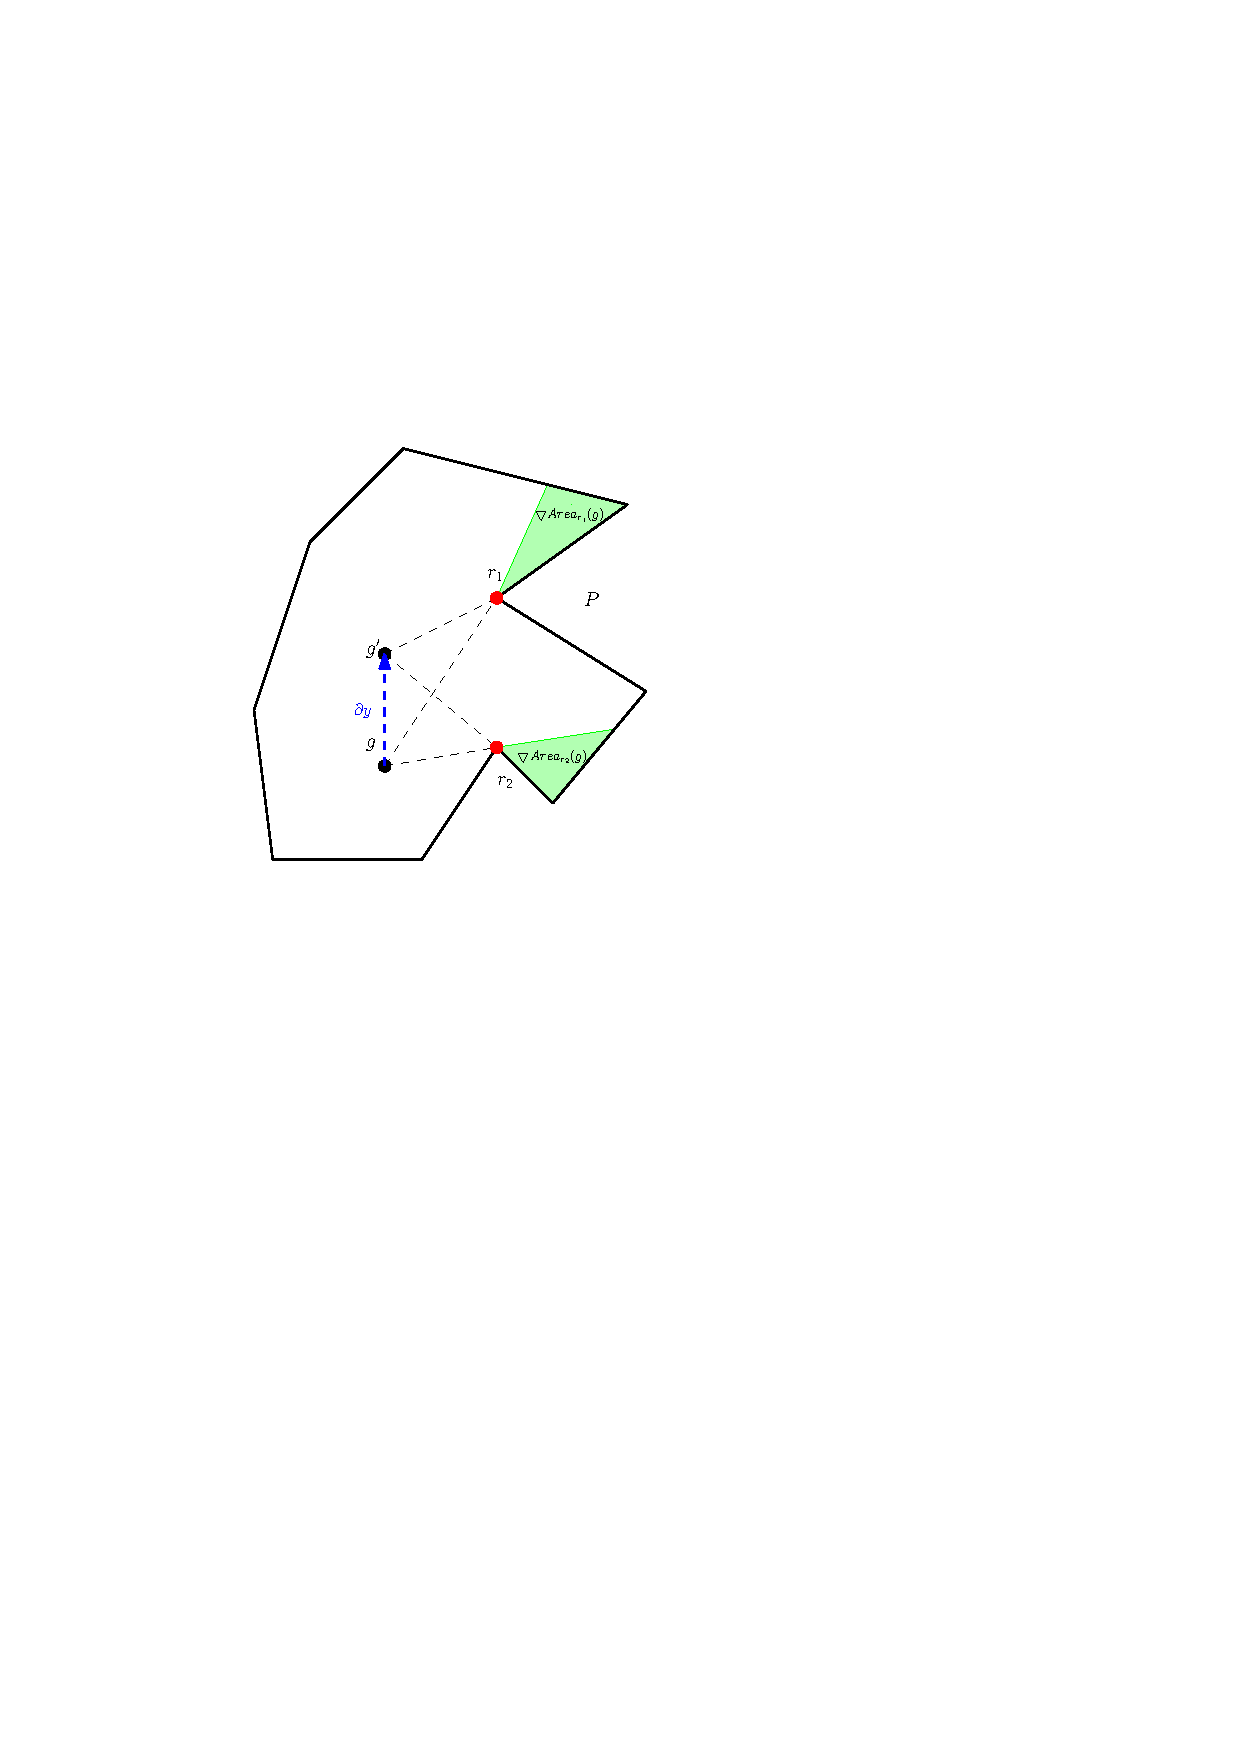
\includegraphics{theory/sumf.pdf}
    \caption{Global change in the area seen by $g$ when moved by $\partial y$ to a new position $g'$.}
    \label{fig:sumf}
\end{figure}


Let $\bigtriangledown f$ be the gradient of $f$. The gradient then indicates the direction of the steepest descent for the objective function $f(g)$.
The learning rate (step size) $\alpha$ is the size of the steps taken to reach the optimum. It is typically a small value, and it is evaluated and chosen based on the behaviour of the optimisation function. 

After the gradient $\bigtriangledown f$ is computed, we  use it to calculate the new optimised position $g'$ of guard $g$: $$g' = g + \alpha\bigtriangledown f(g).$$


In later sections we experiment with various learning rates. As such, we  explore how they influence the performance of our algorithm in relation to different test polygons. 

% \newpage
\subsubsection{Computing the Gradient}

Given that $f$ is a function that describes the visibility area of a point $g$, we first need to define how its gradient is computed. We  simplify the gradient computation without losing generality. As such, we  rotate the plane with rotation matrix $R$, so that $g$ and any reflex vertex $r$ have the same $x$-coordinate. In this way, we only need to compute the gradient when we vary the $y$-coordinate. The computation of the gradient remains the same regardless of the rotation applied to the plane.


We  use the notation $\frac{\partial f}{\partial y}$ to denote the change in the visibility area $f(g)$ when the plane is rotated and then the $y$-coordinate is modified by a small amount $\partial y \rightarrow 0$. In this way, we define 

\begin{equation}
    \bigtriangledown f(g) = \left(\frac{\partial f}{\partial x}, \frac{\partial f}{\partial y}\right)^\intercal \label{eq:gradient}
\end{equation}

to be the gradient of $f$ given that $P$ is guarded by a point $g$. 

We  now create a canonical geometric construction that allows us to further define and compute $\bigtriangledown f$. In this case, we consider the normalised length of the gradient as $||~\bigtriangledown~f(g)||~=~1$. This canonical construction is displayed in Figure \ref{fig:gradient}. 
% We will then generalise this case to multiple reflex vertices and guards.

\begin{figure}[h!]
    \centering
    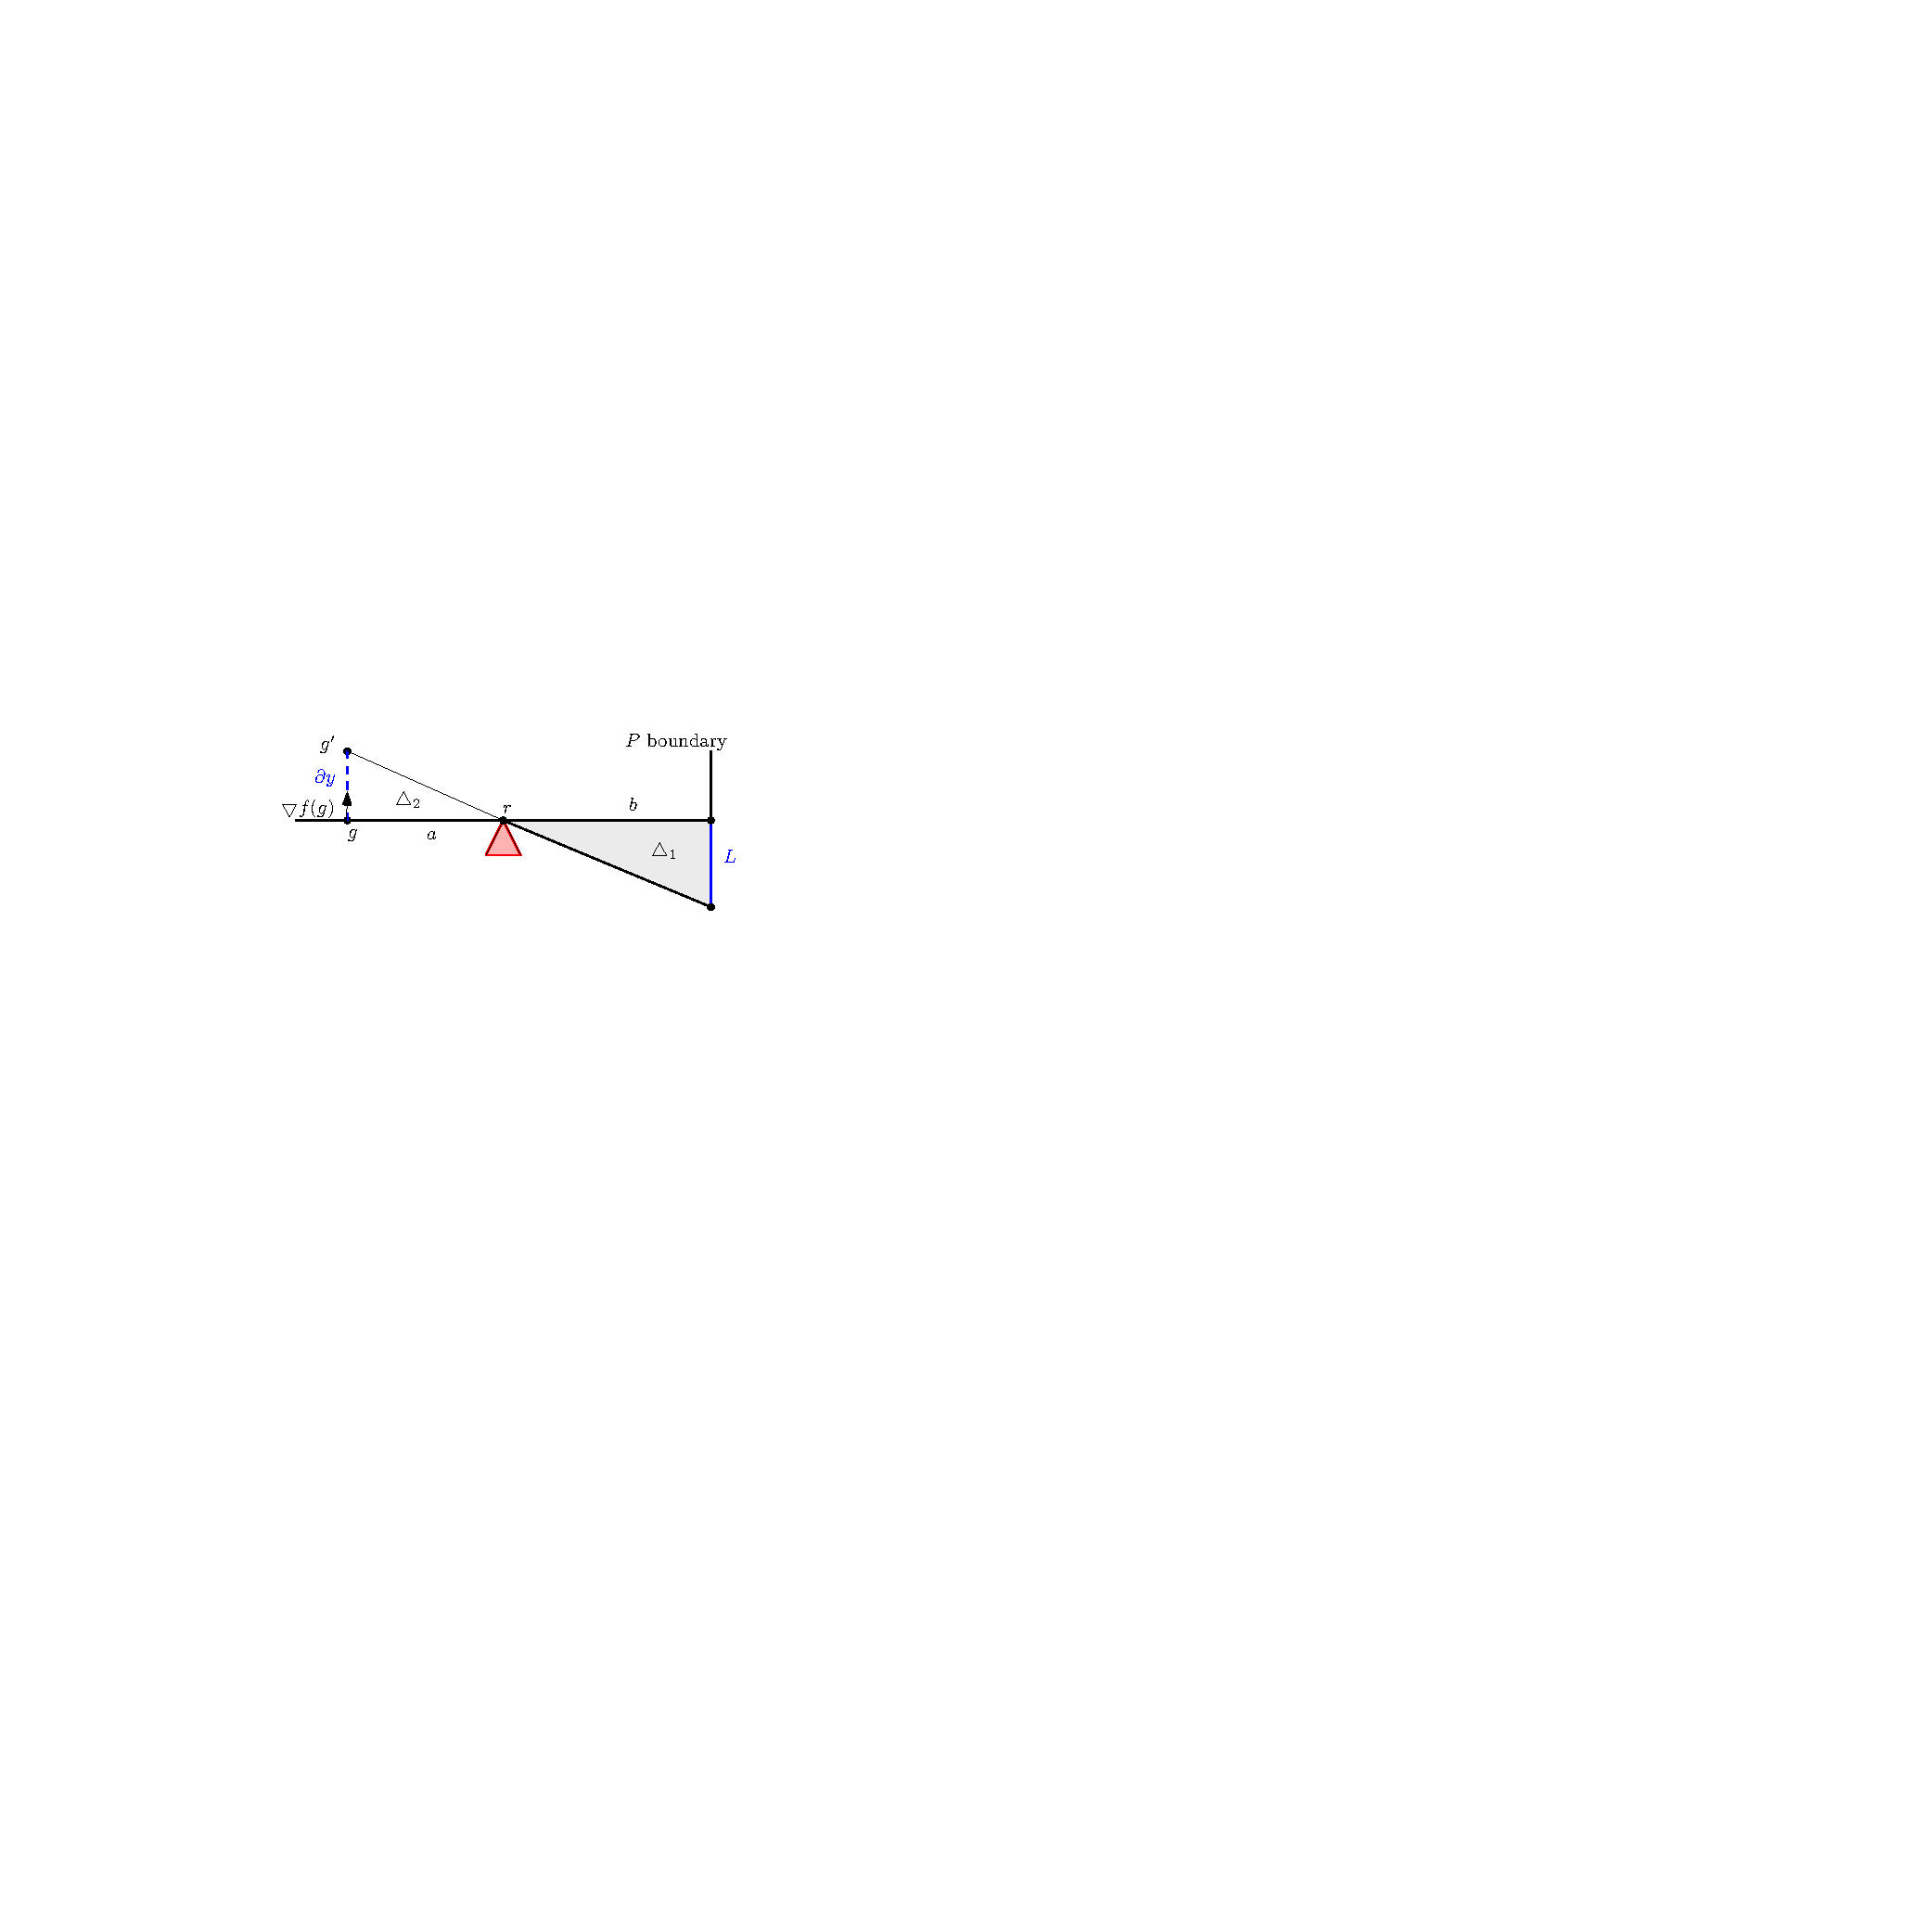
\includegraphics{theory/gradient2.pdf}
    \caption{Canonical gradient construction for when the position of $g$ is varied by a small amount $\partial y$ around reflex vertex $r$ to the new position $g'$.}
    \label{fig:gradient}
\end{figure}

Take a boundary line segment of $P$, $r$ a reflex vertex inside $P$ and $g$ a guard whose optimal position we are interested in. The reflex vertex $r$ is seen by $g$. Let $\overline{gr} = a$ be known, and let $\triangle rgg' = \triangle_2$. Similarly, let $b$ be the known distance between $r$ and the polygon boundary in question.


Let $\partial y$ be a tiny change in the $y$-coordinate of $g$. Let $g'$ be the new position of $g$ given the change $\partial y$. The point $g'$ sees more around $r$ on the polygon boundary. Let $L$ be the new segment that $g'$ sees on the polygon boundary. As such, let $\triangle_1$ denote the increase in the visibility area of $g$ when it moves to position $g'$:

\begin{equation}
    \bigtriangledown \text{Area}_r(g) = \triangle_1. \label{eq:derivative}
\end{equation}

We are now interested in computing how the area seen by guard $g$ increases given the change $\partial y$ in the position of $g$. The distances $a$ and $b$ are known. As such, we aim at expressing the gradient $\bigtriangledown \text{Area}_r$ for point $g$ and reflex vertex $r \in \mathit{Vis}(g)$ using $a$ and $b$. Since $\bigtriangledown \text{Area}_r$ depends on the change in the coordinates of $g$, computing it is tightly connected to the change in the area of triangle $\triangle_1$. We  proceed to calculate the area of $\triangle_1$ below.

Given that triangles $\triangle_1$ and $\triangle_2$ are square triangles, their areas is calculated as:

\begin{align*}
    \text{Area}_{\triangle_1}(g) &= \frac{b L}{2},\\ 
    \text{Area}_{\triangle_2}(g) &= \frac{a \partial y}{2}.
\end{align*}


Given that $\overline{gg'}$ is parallel to polygon's boundary, we  use Thales's Theorem \cite{allman1889greek} in triangles $\triangle_1$ and $\triangle_2$ to compute the length $L$: 

\begin{align}
    % \frac{||\overline{pp'}||}{||\overline{dd'}||} &= \frac a b \\
    \frac{\partial y}{L} &= \frac a b \nonumber \\ 
    L &= \frac{b \partial y}{a}. \label{eq:L}
\end{align}

So, the area of $\triangle_1$ is computed:
\begin{align}
    \text{Area}_{\triangle_1}(g) &= \frac{Lb}{2} \nonumber \\ 
    &\overset{(\ref{eq:L})}{=} \frac{\frac{b \partial y}{a}b}{2} \nonumber \\ 
    \text{Area}_{\triangle_1}(g) &= \frac{b^2 \partial y}{2a}. \label{eq:ardd}
\end{align}

We compute the gradient $\bigtriangledown \text{Area}_r$ in a plane rotated by $R$ for a point $g$ and a reflex guard $r$ seen by $g$ as

\begin{align}
    R\bigtriangledown \text{Area}_r(g) \overset{(\ref{eq:gradient})}{=} &\left(\frac{\partial f}{\partial x}, \frac{\partial f}{\partial y}\right)^\intercal \nonumber \\
    \overset{(\ref{eq:derivative})}{=} &\left(0, \frac{\text{Area}_{\triangle_1}}{\partial y}\right)^\intercal \nonumber \\
    R\bigtriangledown \text{Area}_r(g) \overset{(\ref{eq:ardd})}{=} &\left(0, \frac{b^2}{2a}\right)^\intercal. \label{eq:normf1}
    % \bigtriangledown \text{Area}_r = &\left(0, \frac{b^2}{2a}\right)^\intercal.
\end{align}

% Analogously, if we rotate the plane such that $p$ and reflex vertex $r$ have the same $y$-coordinate, the gradient becomes $$\bigtriangledown f = (\frac{b^2}{2a}, 0)^\intercal.$$

Therefore, for all the reflex vertices $r$ guard $g$ sees, the total gradient $\bigtriangledown f$ becomes the sum of all the partial gradients $\bigtriangledown f_r$ as 
\begin{align}
    \bigtriangledown f(g) &= \sum_{i \in R(g)} \bigtriangledown \text{Area}_i(g), \label{eq:normf2} \\ 
    R(g) &= \{\text{reflex vertices of } P \text{ seen by }g\}. \nonumber
\end{align}

\subsubsection{Computing the New Guard's Position}
We use the coordinates of the gradient $\bigtriangledown f$ to compute the movement direction of the guard $g$ given all the reflex vertices from $P$ seen by $g$. In order to do so, we  use the construction depicted in Figure \ref{fig:vperp}. 

\begin{figure}[h!]
    \centering
    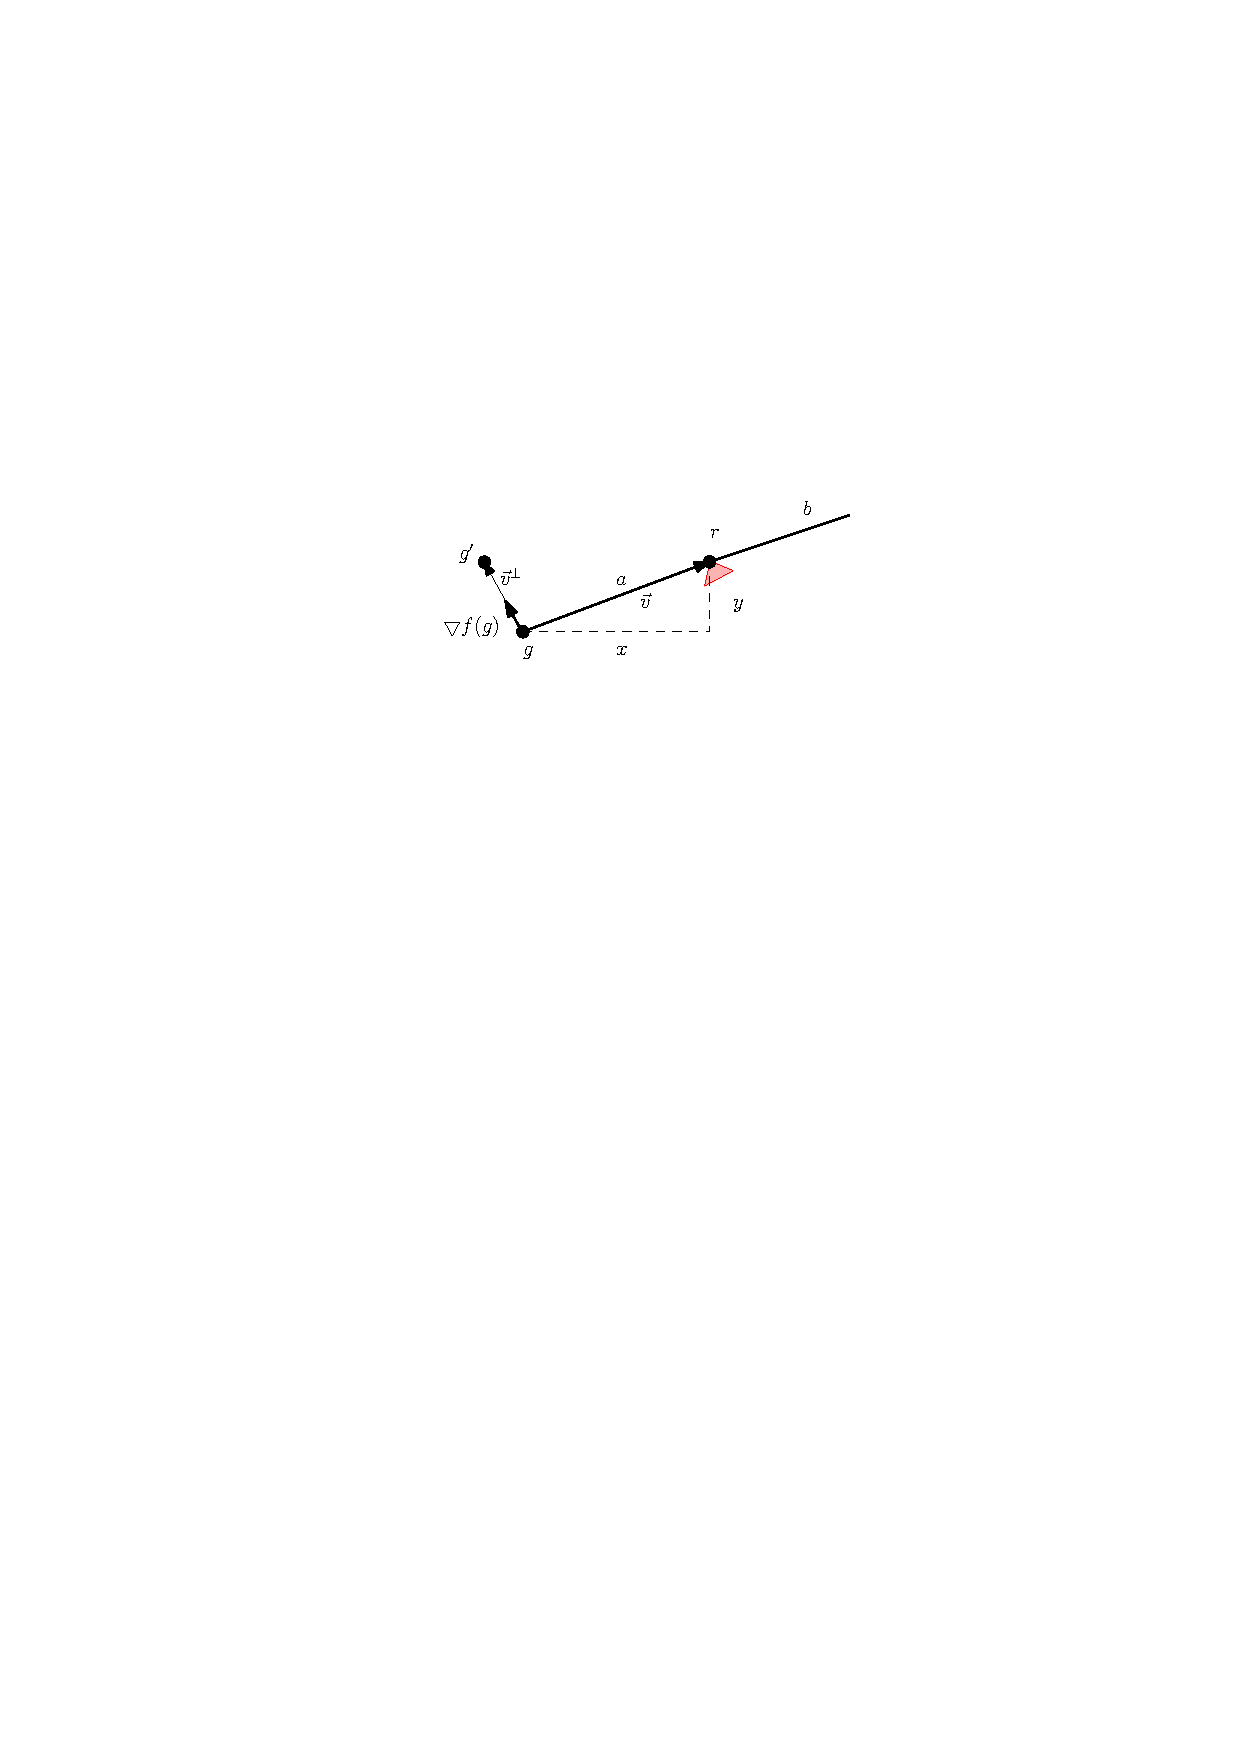
\includegraphics{theory/v_perp.pdf}
    \caption{Computing the new position $g'$ of guard $g$ around reflex vertex $r$ based on the gradient $\bigtriangledown f$.}
    \label{fig:vperp}
\end{figure}

Let $\vec v$ be the vector corresponding to the direction of movement from guard $g$ to a reflex vertex $r$, such that $\vec{v} = (r - g) = (x, y)^\intercal$, with norm $||\vec{v}|| = a$. So, $||\frac{\vec v}{a}|| = 1$.

Let $\vec{v}^\perp  = (g' - g)$ be the vector corresponding to the direction of movement from guard $g$ to its new position $g'$. Vector $\vec v^\perp$ is orthogonal to $\vec{v}$, in the same direction as $\bigtriangledown f$, such that $||\vec{v}|| = ||\vec{v}^\perp|| = a$. We  use the coordinates of $\vec{v}^\perp$ to compute the coordinates of $\bigtriangledown f$ and thus the direction in which $g$ needs to move.

The coordinates of $\vec v^\perp$ are computed using the construction from Figure \ref{fig:vsquare}. Since $\vec v^\perp \perp \vec v$, and $g$ and $r$ are on the right-hand side of $\vec v^\perp$, the coordinates of $\vec v^\perp$ are rotated by $-90^\circ$ so that $\vec v^\perp = (-y, x)^\intercal$. Analogously for the case when $g$ and $r$ are rotated by $180^\circ$ to the left-hand side of $\vec v^\perp$, the coordinates of $\vec v^\perp$ are rotated by $90^\circ$ to $\vec v^\perp = (-x, y)^\intercal$.

\begin{figure}[h!]
    \centering
    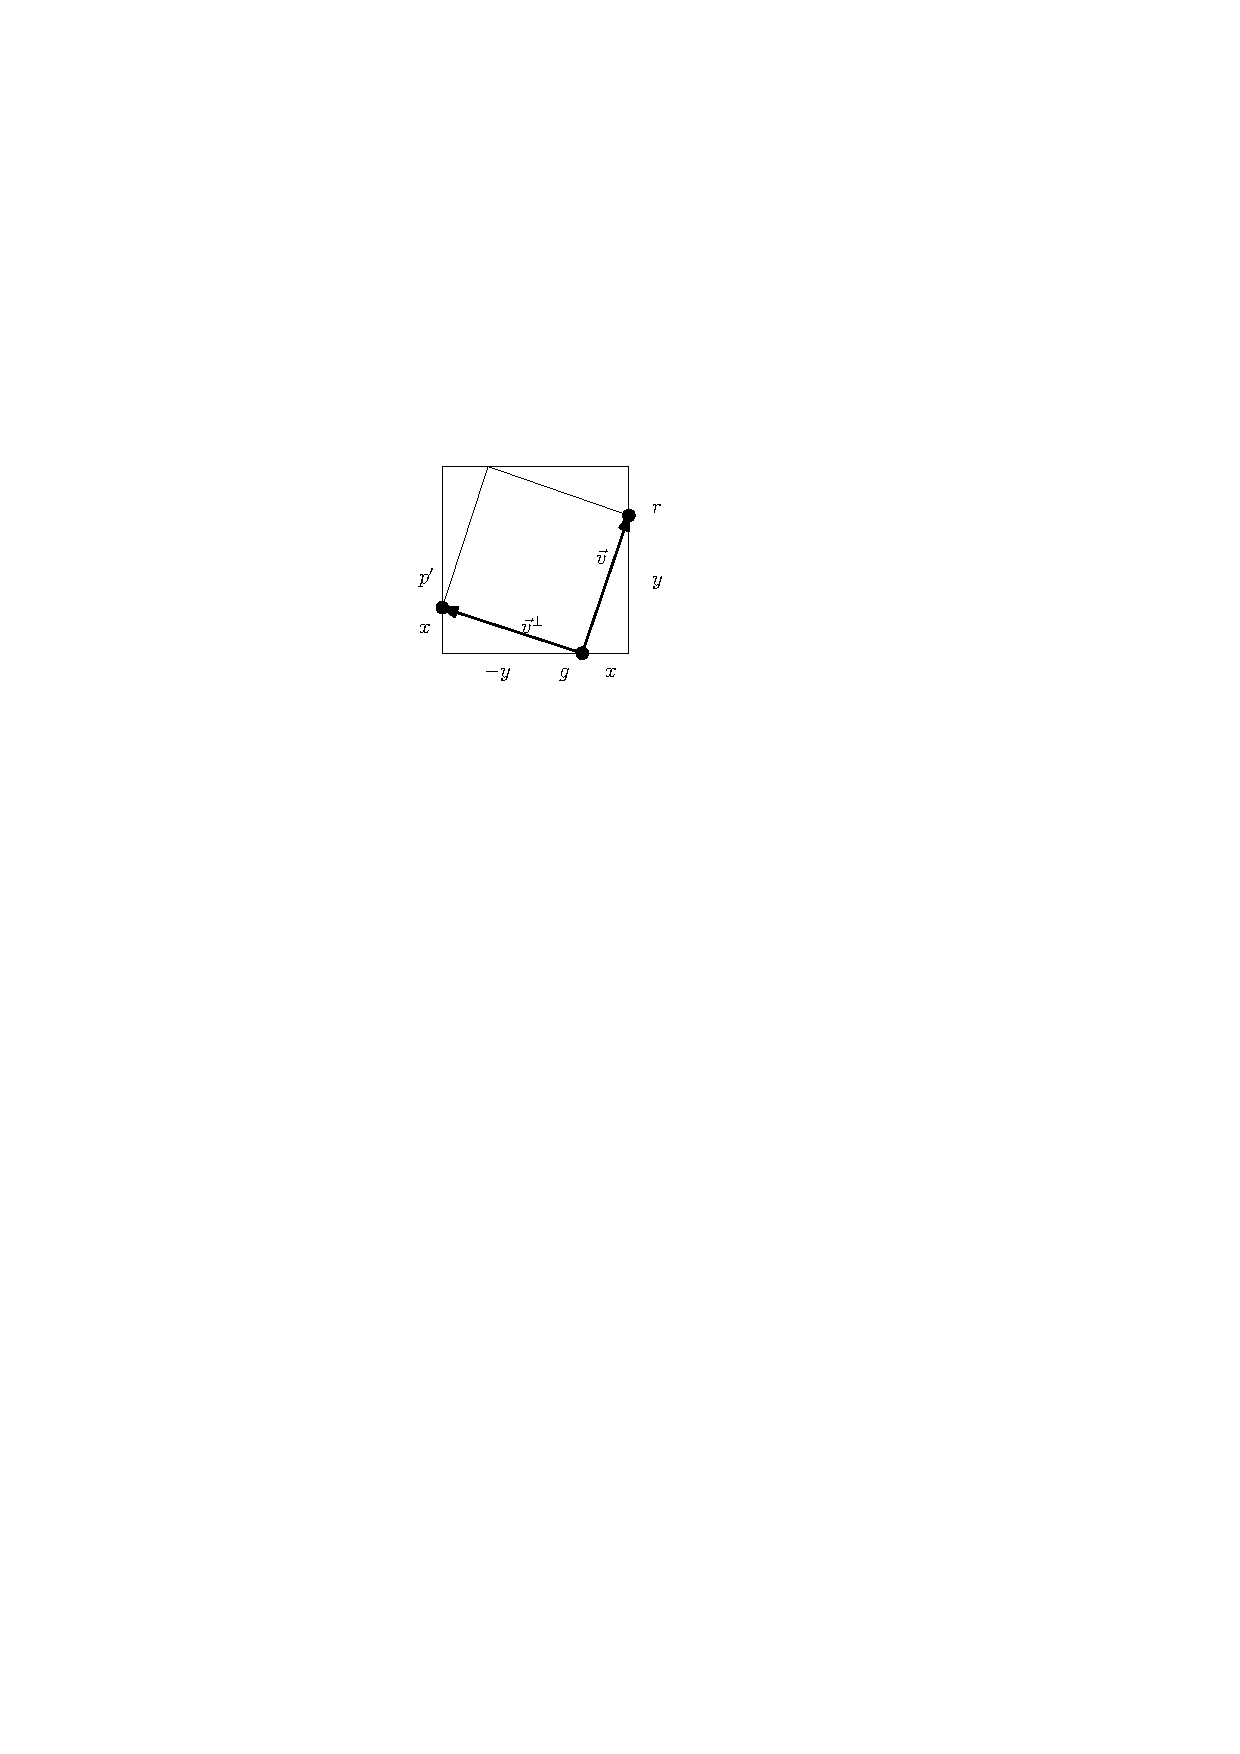
\includegraphics{theory/v_square.pdf}
    \caption{Computing the coordinates of $\vec v^\perp$ given the guard $g$ and the reflex vertex $r = (x, y)$.}
    \label{fig:vsquare}
\end{figure}

We know that the norm of the total gradient $\bigtriangledown f$ is 
\begin{align}
    ||\bigtriangledown f(g)|| \overset{(\ref{eq:normf2})}{=} &||\sum \left(0, \frac{b^2}{2a}\right)^\intercal|| \nonumber \\
    \overset{(\ref{eq:normf1})}{=} &\sqrt{\left(\frac{b^2}{2a}\right)^2} \nonumber \\
    ||\bigtriangledown f(g)|| = &\frac{b^2}{2a}. \label{eq:normf}
\end{align}

Since $\bigtriangledown f$ has the same direction as $\vec v^\perp$, we wish to normalise it with $\frac 1 a$ (the norm of $\vec v^\perp$). Therefore, the gradient for guard $g$ and one reflex vertex $r \in \mathit{Vis}(g)$ is computed as 
\begin{align}
    \bigtriangledown f(g) = \vec v^\perp \frac{b^2}{2a} \frac 1 a. \label{eq:f}
\end{align}

As mentioned before, the total gradient for guard $g$ and all the reflex vertices $r$ the guard sees is 
\begin{align*}
    \bigtriangledown f(g) &= \sum_{r \in R(g)} \bigtriangledown \text{Area}_r, \\
    R(g) &= \{\text{reflex vertices of } P \text{ seen by }g\}.
\end{align*}

The new position $g'$ of guard $g$ based on all the reflex vertices it sees is: 
\begin{equation}
    g' = g + \alpha\bigtriangledown f(g).
    \label{eq:l}
\end{equation}

% \newpage
\subsection{Guarding the Polygon with Multiple Guards}
In this section we  investigate how to generalise the computation of gradient descent to multiple guards. Previously we defined the gradient descent of one guard in order to compute its movement towards optimality. We extend this computation to multiple guards. Namely, we define how the gradient descent changes when the visibility region of one guard is seen by other guards as well.

\subsubsection{Computing the Gradient for Two Guards}
Let point $g_1$ be the guard we have previously computed the gradient for. Let point $g_2$ be another guard in the polygon. The position of $g_2$ is optimised around reflex vertex $r_2$, as seen in Figure \ref{fig:poly_gradient}. Guard $g_2$ sees a part of the visibility region already seen by $g_1$. Let the shared seen region be $\triangle_2$, and the region that is only visible by $g_1$ be $\triangle_1$.

\begin{figure}[h!]
    \centering
    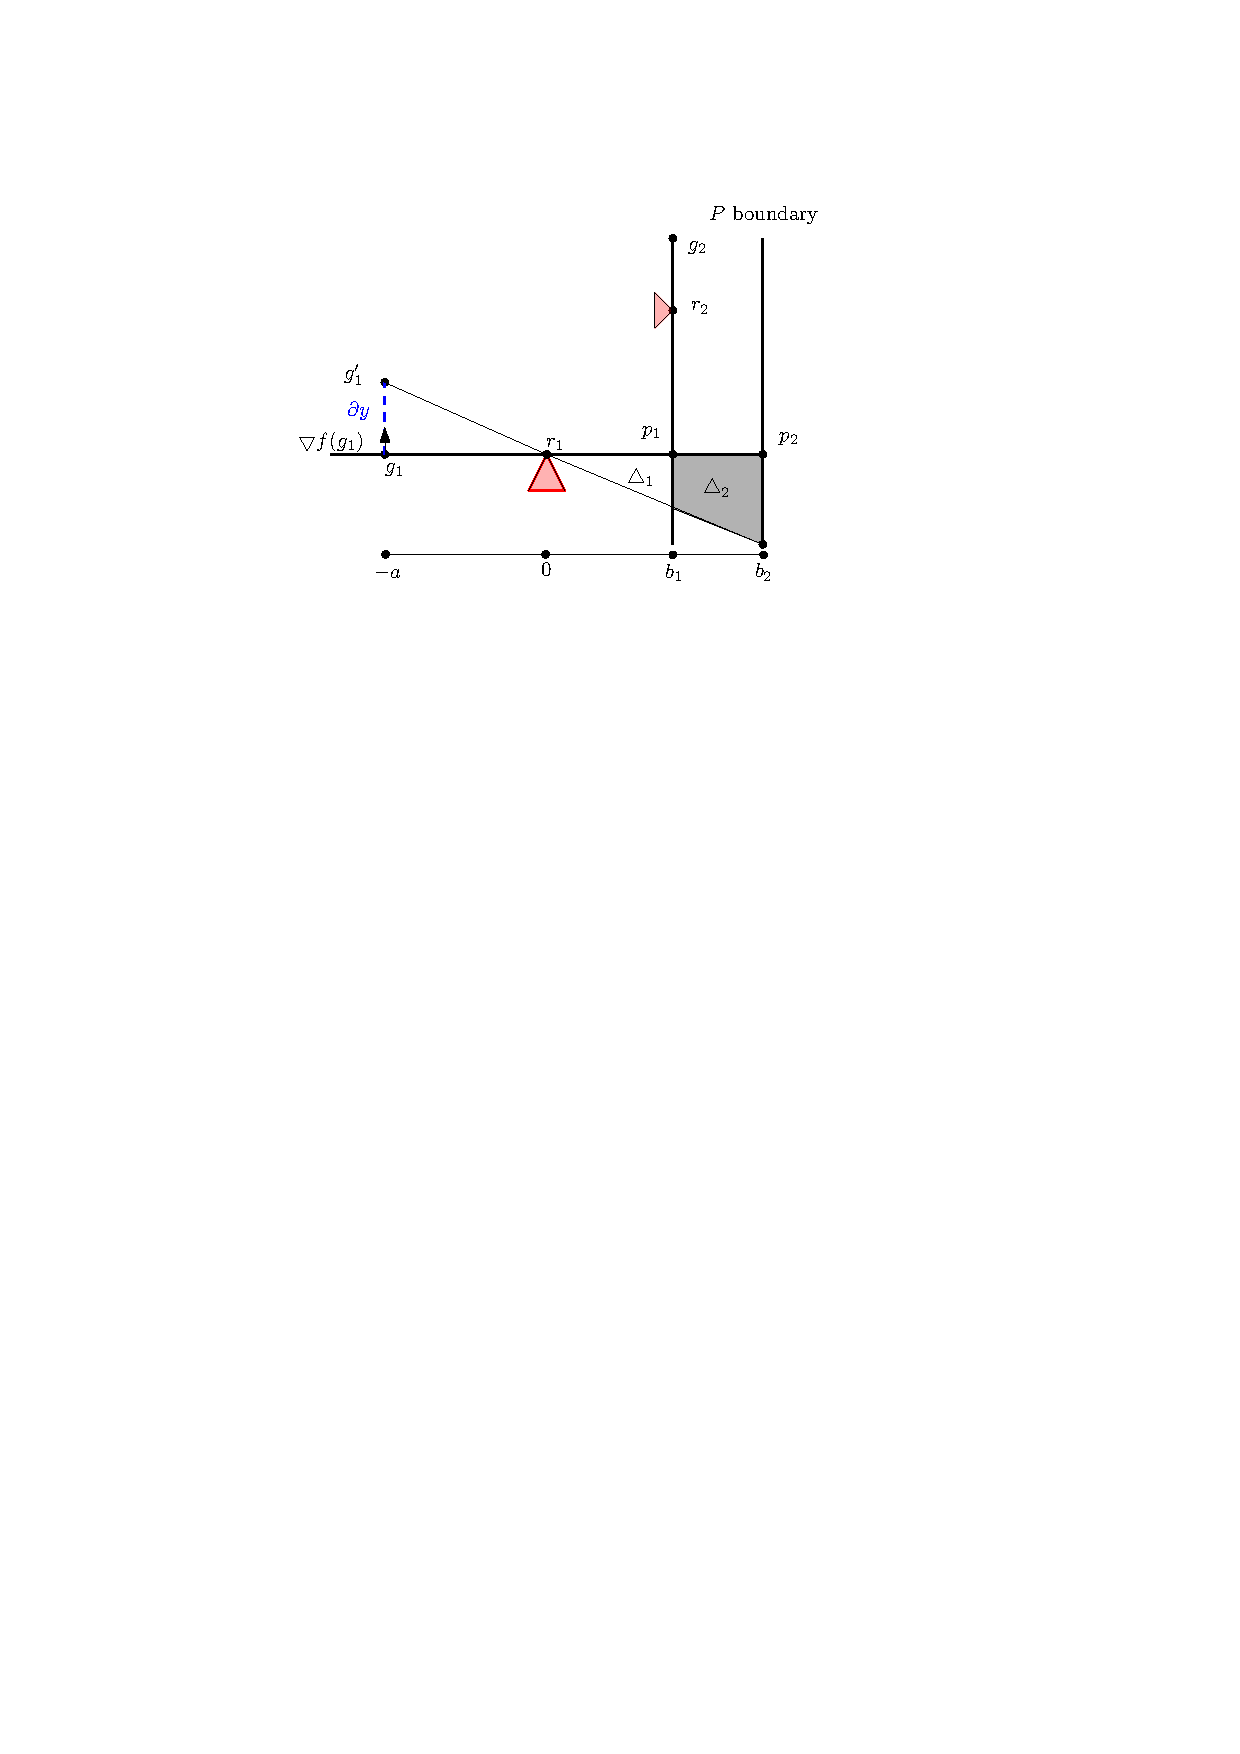
\includegraphics{theory/gradient3.pdf}
    \caption{Canonical gradient construction for when the visible area of $g_1'$ is also seen by guard $g_2$.}
    \label{fig:poly_gradient}
\end{figure}

The visibility regions of guards $g_1$ and $g_2$ are computed. Let $p$ be the intersection point between them. Let $d$ be the point seen by $g_1$ on the polygon boundary. Point $p$ divides the segment seen by $g_1$ behind the reflex vertex $r_1$ into two subsegments $\overline{r_1p_1}$ and $\overline{p_1p_2}$. The lengths of the subsegments are $b_1$ and $b_2$, respectively, with $b_1 + b_2 = b$. Recall that $b$ is the distance between the reflex vertex $r_1$ and the polygon boundary. Thus,  $b_2$ corresponds to the length of the shared seen segment.

As before in equation \ref{eq:ardd}, the area seen by $g_1$ is $$\text{Area}_{\triangle_1 + \triangle_2}(g_1) = (b_1 + b_2)^2\frac{\partial y}{2a}.$$
However, $\triangle_2$ is already seen by guard $g_2$. Since this area is already covered, we are only interested in how $g_1$ covers the remaining $\triangle_1$. 
We can compute that from the same equation as $$\text{Area}_{\triangle_1}(g_1) = b_1^2\frac{\partial y}{2a}.$$
So, we do not need to take $\triangle_2$ into account when computing the gradient of $g_1$. 
% We thus need to subtract the area of $\triangle_2$ from the total area seen by $g_1$. 

Now we can also compute the shared area seen $\triangle_2$ as:
\begin{align}
    \text{Area}_{\triangle_2}(g_1) &= \text{Area}_{\triangle_1 + \triangle_2}(g_1) - \text{Area}_{\triangle_1}(g_1) \nonumber \\
                              &= (b_1 + b_2)^2\frac{\partial y}{2a} - b_1^2\frac{\partial y}{2a} \nonumber \\
    \text{Area}_{\triangle_2}(g_1)&= \left[(b_1 + b_2)^2 - b_1^2\right]\frac{\partial y}{2a}. \label{eq:multiple_areas} 
\end{align}

We use thus equation \ref{eq:multiple_areas} in the next section to introduce a generalisation for the computation for the exclusive area seen by $g_1$.
% Then, we  compute the area $\triangle_1$ seen exclusively by $g_1$ by subtracting the shared area of $\triangle_2$ from the total area seen by $g_1$: 
% \begin{align*}
%     \text{Area}_{\triangle_1}(g_1) &= \text{Area}_{\triangle_1 + \triangle_2}(g_1) - \text{Area}_{\triangle_2}(g_1) \\
%                               &= (b_1 + b_2)^2\frac{\partial y}{2a} - \left[(b_1 + b_2)^2 - b_1^2\right]\frac{\partial y}{2a} \\
%     \text{Area}_{\triangle_1}(g_1) &= b_1^2\frac{\partial y}{2a}. 
% \end{align*}

\subsubsection{Computing the Gradient for Multiple Guards}
We generalise the gradient computation to $m$ guards and $m$ intersection points. Let $g$ be the guard whose position we wish to optimise around reflex vertex $r$ as before. Let the areas highlighted in blue in Figure \ref{fig:general_gradient} be the parts of the visibility region of $g$ that are also seen by the other $m - 1$ guards. Let the visibility region of $g$ intersect other guards' visibility regions in $m$ intersection points $p_1, p_2, ..., p_m$. Let the distance from the reflex vertex $r$ to the intersection points be $b_{1}, b_{2}, ..., b_{m}, b$.

\begin{figure}[h!]
    \centering
    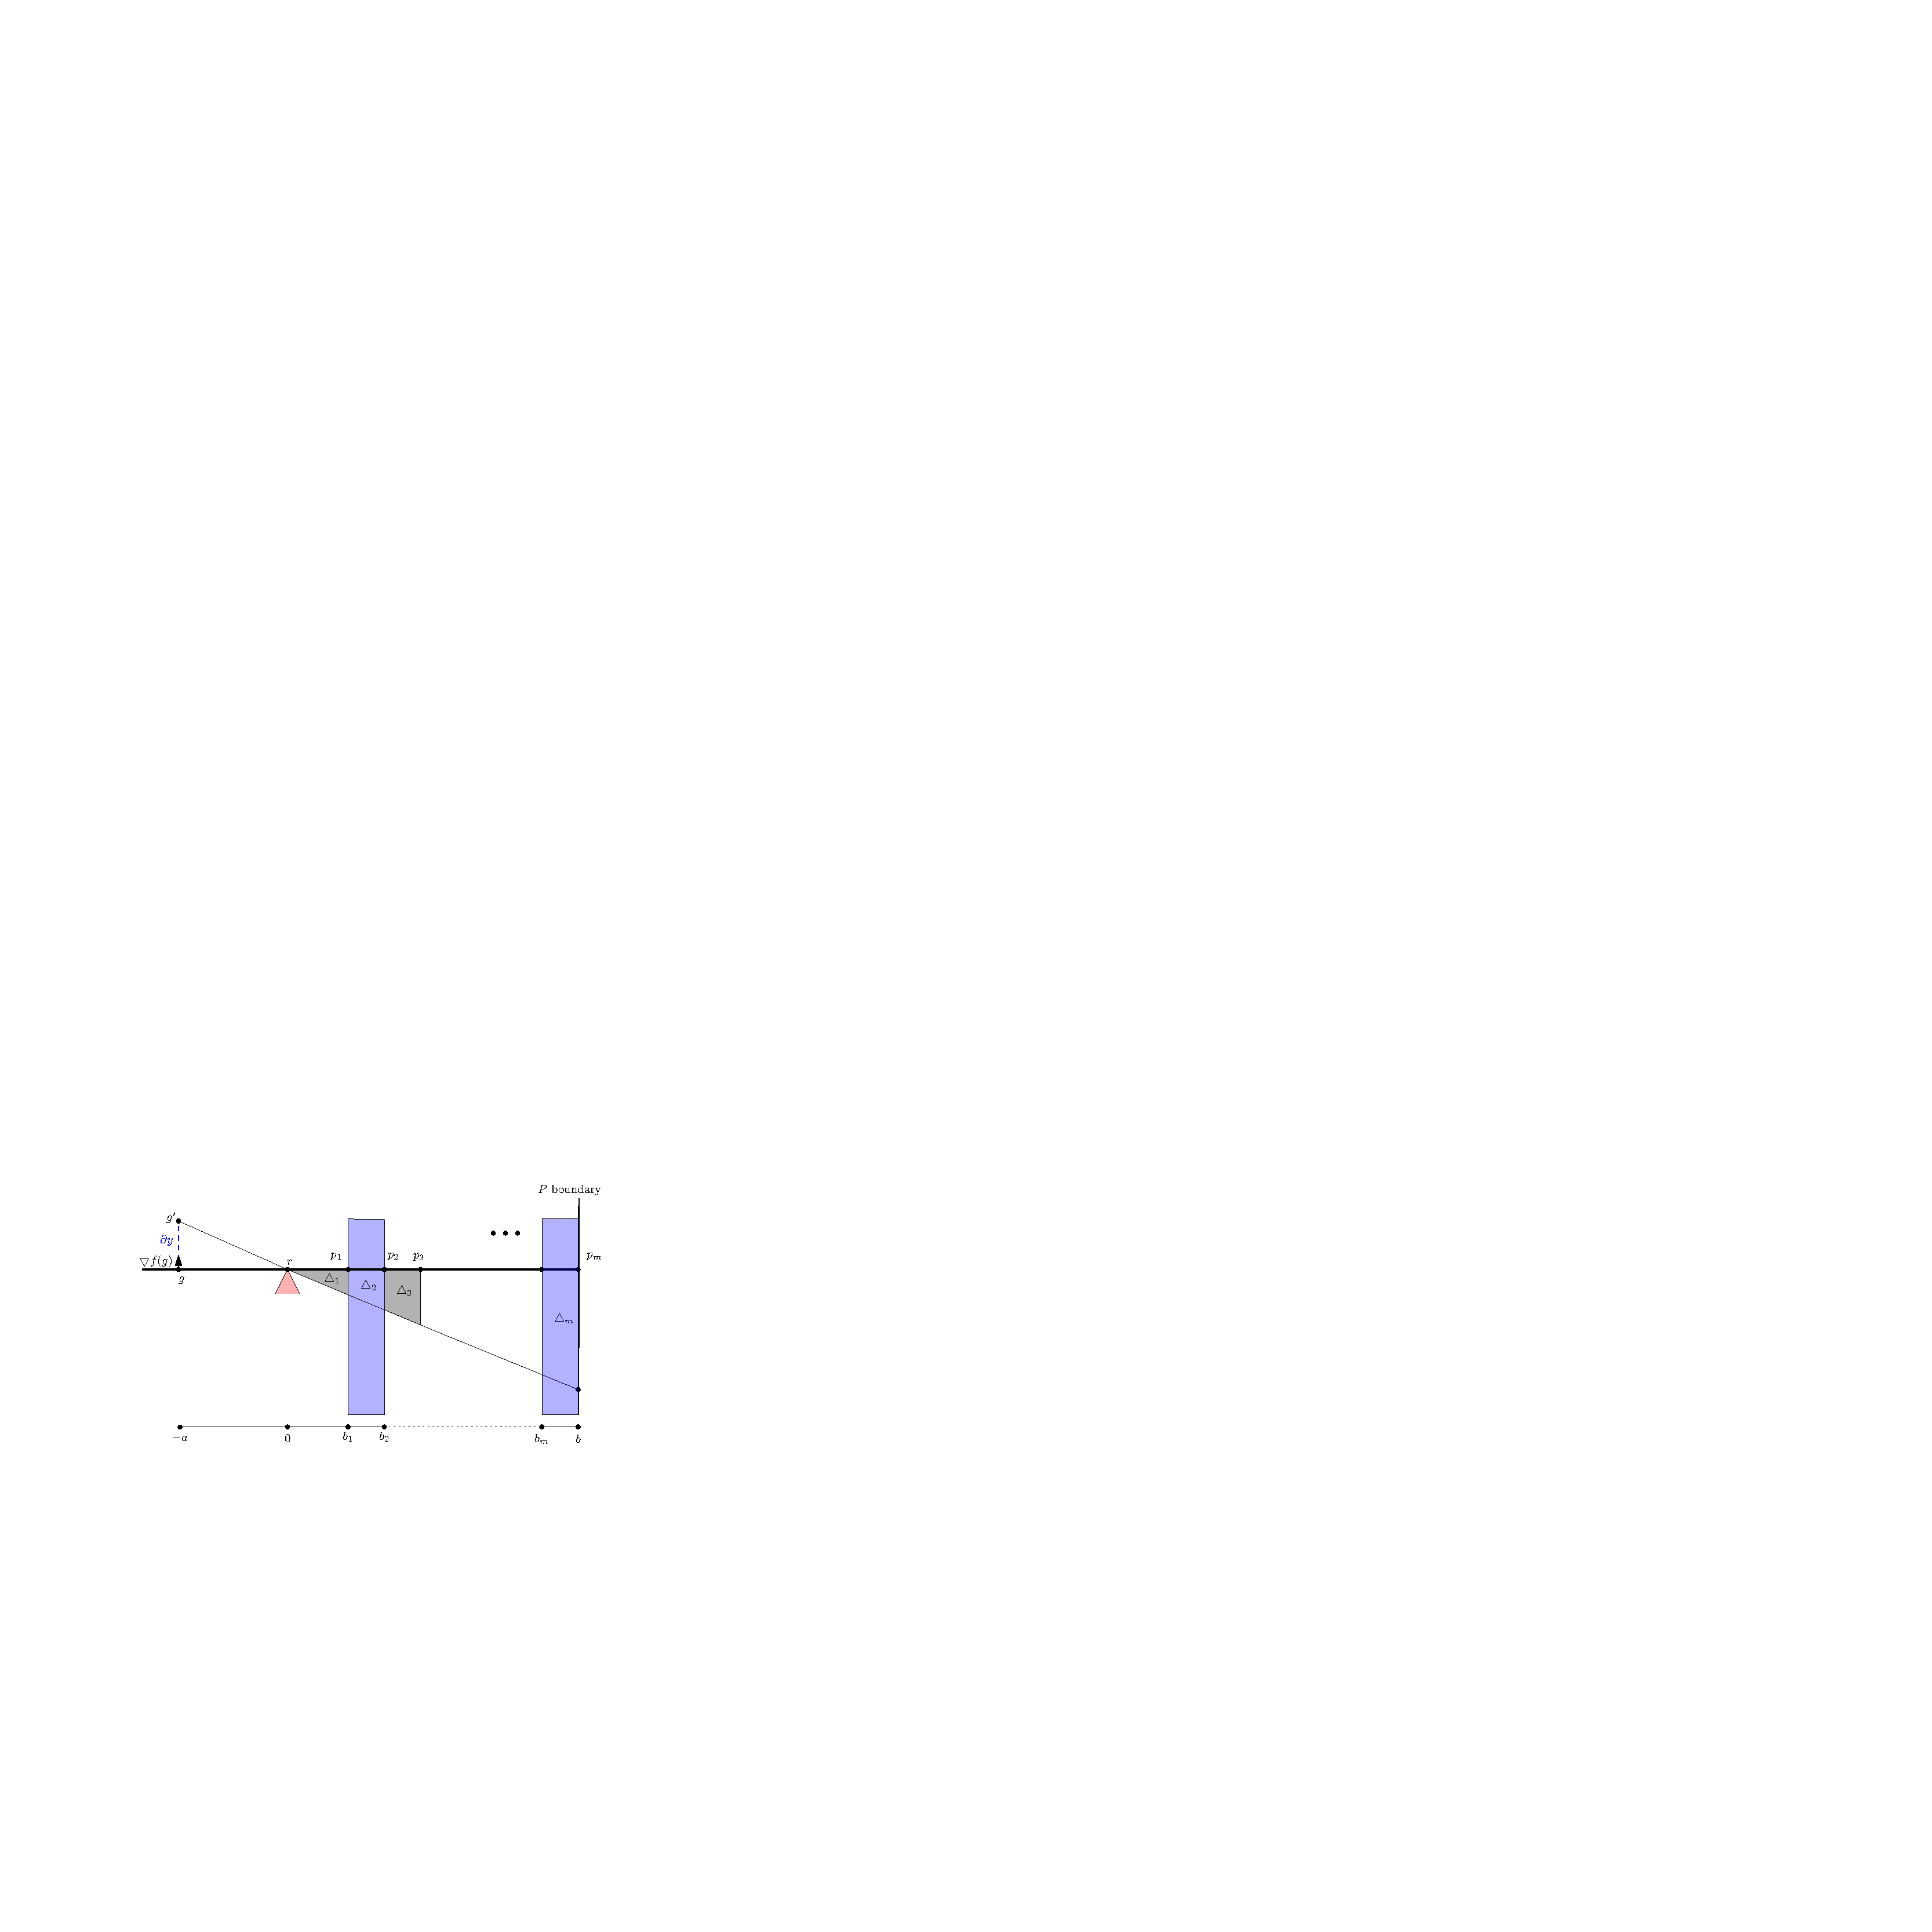
\includegraphics{theory/gradient4.pdf}
    \caption{Canonical gradient construction for where the pink parts of the visible area of $g$ are also seen by other guards. The grey polygons $\triangle_1, \triangle_3, ..., \triangle_{m - 1}$ are the areas that are exclusively seen by $g$.}
    \label{fig:general_gradient} 
\end{figure}

We generalise equation \ref{eq:multiple_areas}. Namely, we need to subtract the areas that are seen by other guards from the total area seen by guard $g$. 

We start to move in the direction from the polygon boundary to reflex vertex $r$. We know the intersection points $p_{m - 1} ..., p_3, p_1$ of the shared seen regions with the visibility region of $g$. Thus, we  compute the distances $\overline{rp_{m - 1}}, ..., \overline{rp_3}, \overline{rp_1}$ between the reflex vertex $r$ and the beginning of the shared visibility regions. Analogously, we  compute the distances $\overline{rp_m}, ...,  \overline{rp_4}, \overline{rp_2}$ between the reflex vertex $r$ and the end of the shared visibility regions.

The areas of polygons $\triangle_1, \triangle_2, ..., \triangle_m$ do not grow linearly. For this reason, we cannot simply subtract the sum of the shared areas from the total area seen by $g$. 

An explanation about why this is the case is given in Figure \ref{fig:areas}. Take overlapping polygons $s_1, s_2, s_3, s_4$ with areas $\text{Area}_{s_1} = 2$, $\text{Area}_{s_2} = 3$, $\text{Area}_{s_3} = 4$, $\text{Area}_{s_4} = 5$. We want to compute the area of polygons $s_1$ and $s_2$. However, it is incorrect to simply add their areas together as $\text{Area}_{s_1 + s_3} = 2 + 4 = 6$, as $s_2$ is overlapping in between them. Instead, from the total area $\text{Area}_{s_1 + s_2 + s_3 + s_4} = \text{Area}_{s_4} = 5$ we  sequentially subtract the areas we are not interested in ($\text{Area}_{s_2}, \text{Area}_{s_4}$) and add the ones we are interested in ($\text{Area}_{s_1}, \text{Area}_{s_3}$). Namely, $\text{Area}_{s_1 + s_3} = \text{Area}_{s_1 + s_2 + s_3 + s_4} - \text{Area}_{s_4} + \text{Area}_{s_3} - \text{Area}_{s_2} + \text{Area}_{s_1} = 5 - 5 + 4 - 3 + 2 = 3$.

\begin{figure}[h!]
    \centering
    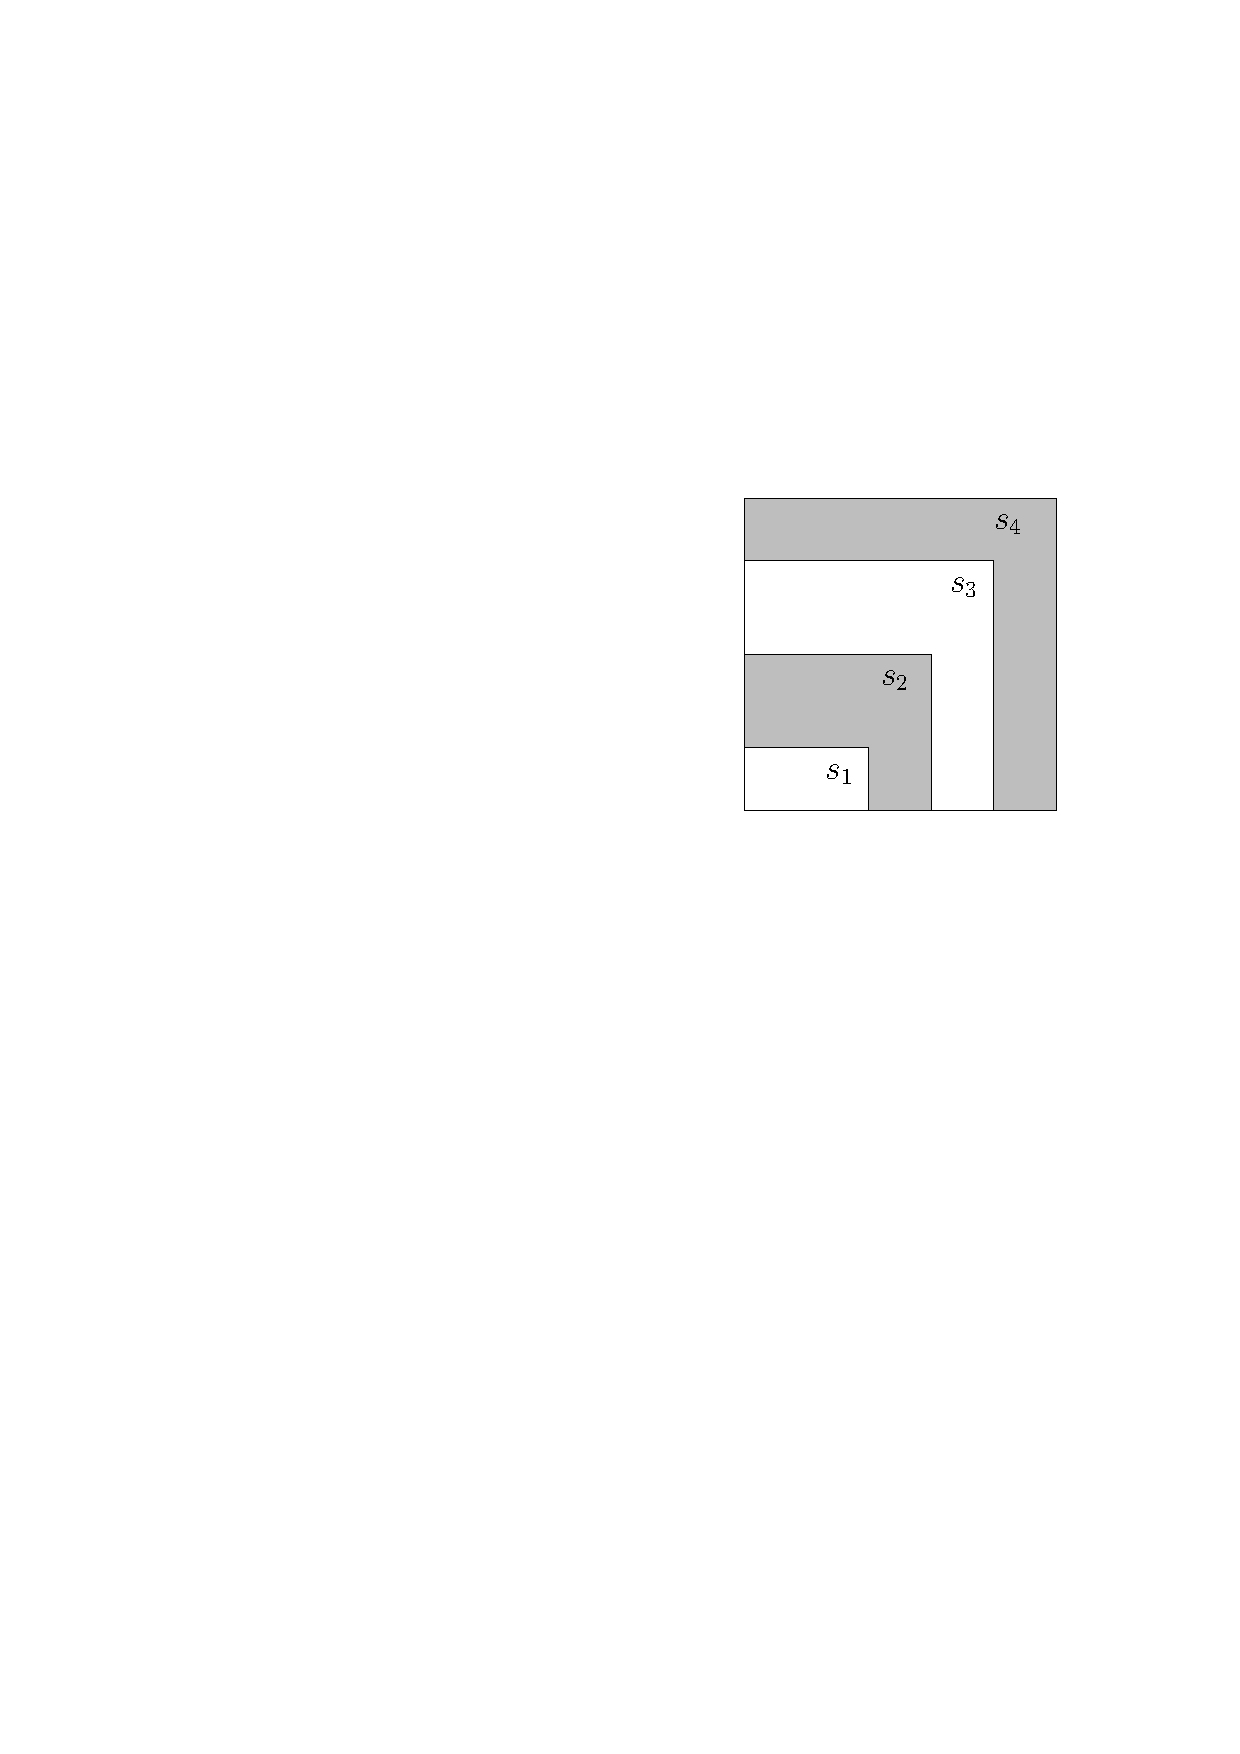
\includegraphics{theory/area.pdf}
    \caption{Example for computing the area of overlapping polygons with areas $\text{Area}_{s_1} = 2$, $\text{Area}_{s_2} = 3$, $\text{Area}_{s_3} = 4$, $\text{Area}_{s_4} = 5$. It is incorrect to compute $\text{Area}_{s_1 + s_3} = 2 + 4 = 6$. Instead, $\text{Area}_{s_1 + s_3} = \text{Area}_{s_1 + s_2 + s_3 + s_4} - \text{Area}_{s_4} + \text{Area}_{s_3} - \text{Area}_{s_2} + \text{Area}_{s_1} = 5 - 5 + 4 - 3 + 2 = 3$.}
    \label{fig:areas}
\end{figure}

Similarly to Figure \ref{fig:areas}, we  compute the area seen exclusively by $g$. From the total area $\text{Area}_{\triangle_1 + \triangle_2, ..., \triangle_m}$ seen by $g$ we need to alternatively subtract the shared areas $\text{Area}_{\triangle_m}, ..., \text{Area}_{\triangle_4},$ $\text{Area}_{\triangle_2}$, then add the exclusively seen areas $\text{Area}_{\triangle_{m - 1}}, ..., \text{Area}_{\triangle_3}, \text{Area}_{\triangle_1}$.

% Figure \ref{fig:general_gradient} displays an example
% For each area seen by multiple guards, we know the length of the subsegments in between reflex vertex $r$ and the shared area beginning and ending, respectively. 
% In order to do so, we need to subtract the area $b_{i + 1}^2$ in between reflex vertex $r$ and the ending of the area, and then add back the area $b_i^2$ between $r$ and the beginning of the area. We need to repeat this process for each of the areas that are shared, in the direction starting from the polygon boundary to the reflex vertex.

This results in the fact that the area seen by $g$ exclusively is computed as 
\begin{align*}
    \text{Area}_{\triangle_1 + \triangle_3 + ... + \triangle_{m - 1}}(g) &= \text{Area}_{\triangle_1 + \triangle_2 + ... + \triangle_m}(g) \\
    &- \text{Area}_{\triangle_{m - 1}}(g) + \text{Area}_{\triangle_{m - 2}}(g) \\
    &- ... \\
    &- \text{Area}_{\triangle_2}(g) + \text{Area}_{\triangle_1}(g) \\
                                                                         &= \left(b^2 - b_{m}^2 + b_{(m - 1)}^2 - ... - b_{2}^2 + b_{1}^2\right)\frac{\partial y}{2a}.
\end{align*}

Alternatively, if $\triangle_1$ is first seen by other guards (so $b_{11} = 0$), then all the signs are flipped. This claim is also supported by the intuition of Figure \ref{fig:areas}. If we are interested in the areas of $s_2$ and $s_4$, then it is incorrect to compute them as $\text{Area}_{s_2 + s_4} = 3 + 5 = 8$. This is because $s_1$ and $s_3$ are overlapping in between them.  Instead, $\text{Area}_{s_2 + s_4} = \text{Area}_{s_1 + s_2 + s_3 + s_4} + \text{Area}_{s_4} - \text{Area}_{s_3} + \text{Area}_{s_2} - \text{Area}_{s_1} = 5 + 5 - 4 + 3 - 2 = 7$.

\subsection{Momentum}
\label{sec:momentum}

This section introduces an extension to the regular gradient descent algorithm: momentum. 
% Its aim is to smoothen out the large noisy jumps in the gradient descent computation \cite{goodfelow2016deep}. 
Momentum builds upon the idea of considering the past states of the gradient descent computation. In this way, the past states create ``inertia'' to the newly computed gradient state. This results in the movement trajectory to be smoother. 
This is especially advantageous for the gradient descent computation. The reason is that the gradient descent computations can be noisy. So some of them are extremely large, while others are insignificant. Momentum addresses this non-uniformity \cite{goodfelow2016deep}.

An example for the benefits of using momentum are found in Figure \ref{fig:momentums}. Subfigure \ref{fig:theory_no_momentum} displays a gradient descent computation without momentum. Initially, the jumps are large and become smaller as the minimum is approached. In Subfigure \ref{fig:theory_momentum} these movements become smoothened out. The gradient descent steps become thus more even. This allows the overall trajectory to be less noisy and chaotic.

\begin{figure}[!h]
    \centering
    \begin{subfigure}{0.45\textwidth}
        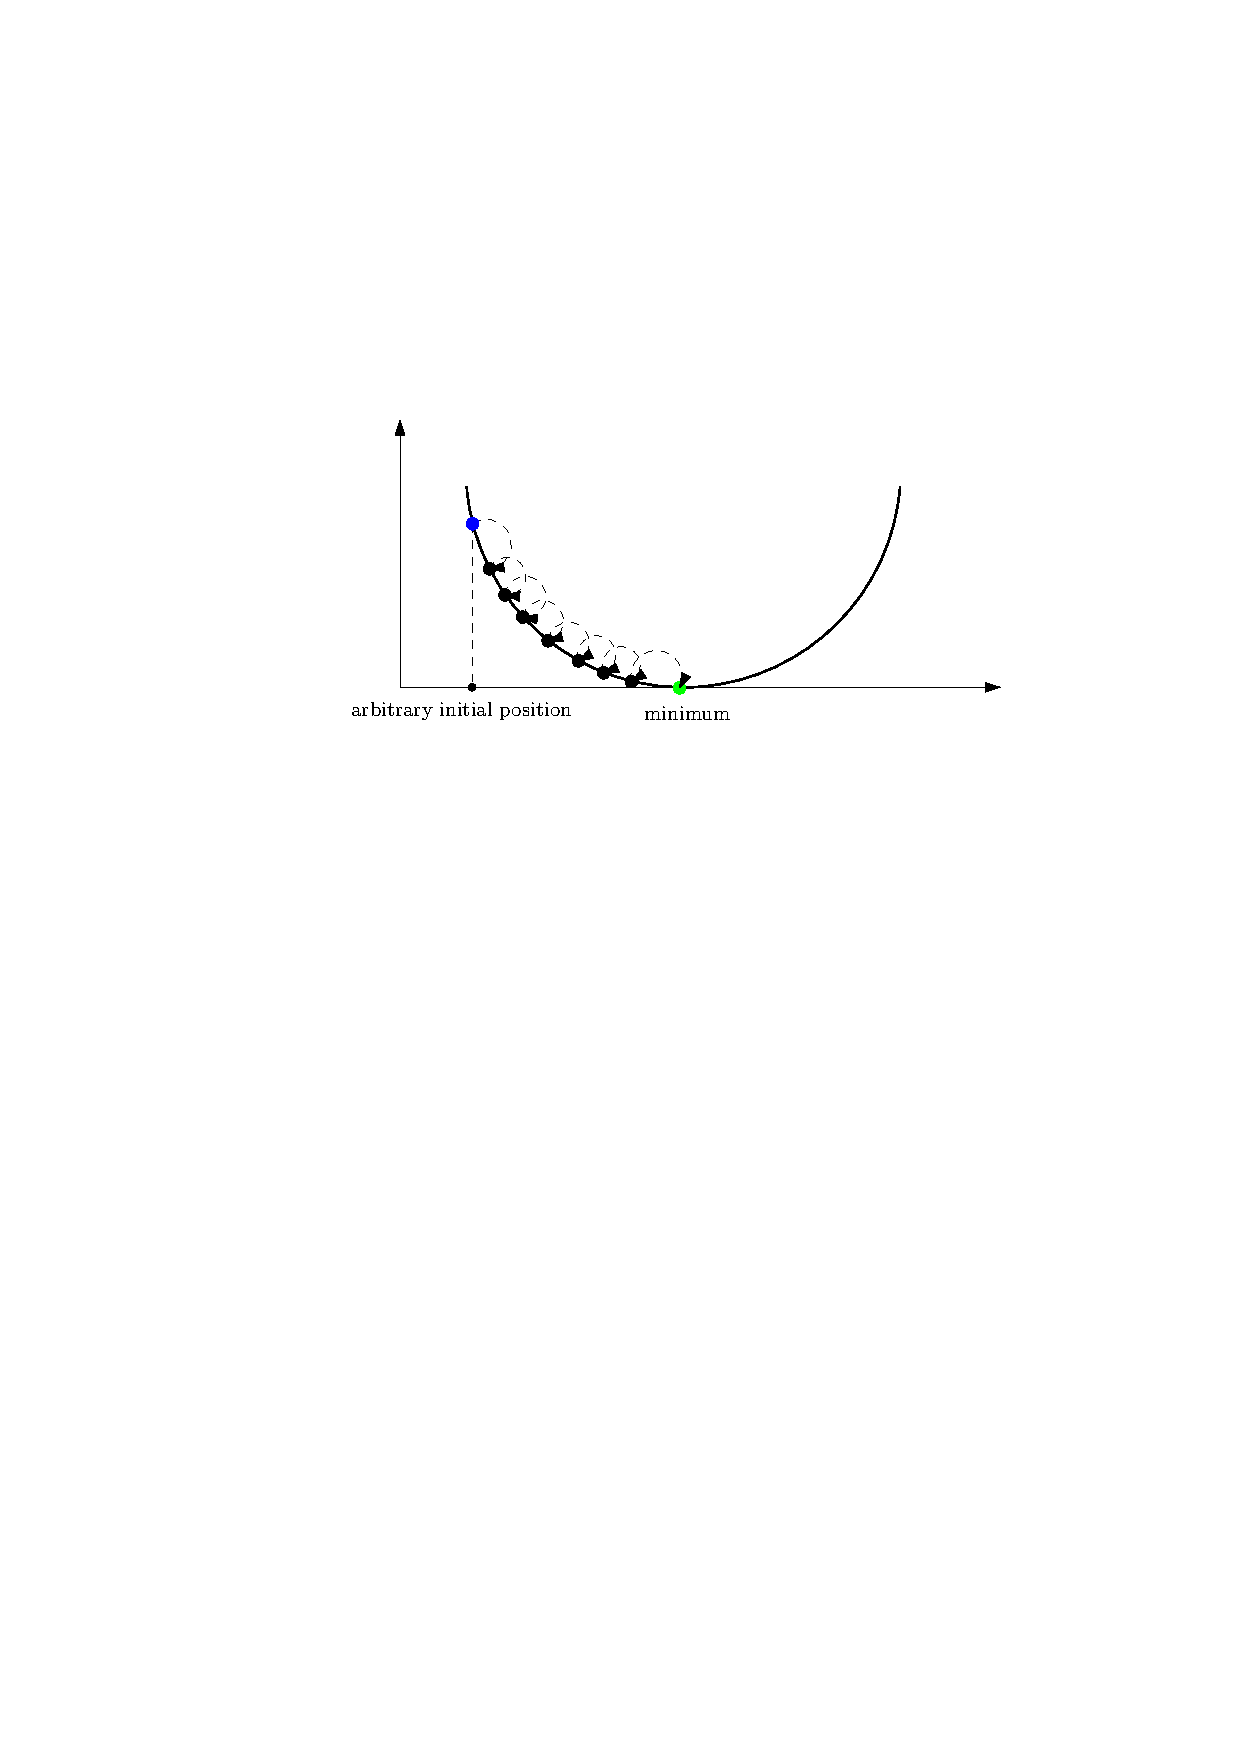
\includegraphics{theory/gradient.pdf}
        \caption{No momentum.}
        \label{fig:theory_no_momentum}
    \end{subfigure}
    \hfill
    \begin{subfigure}{0.45\textwidth}
        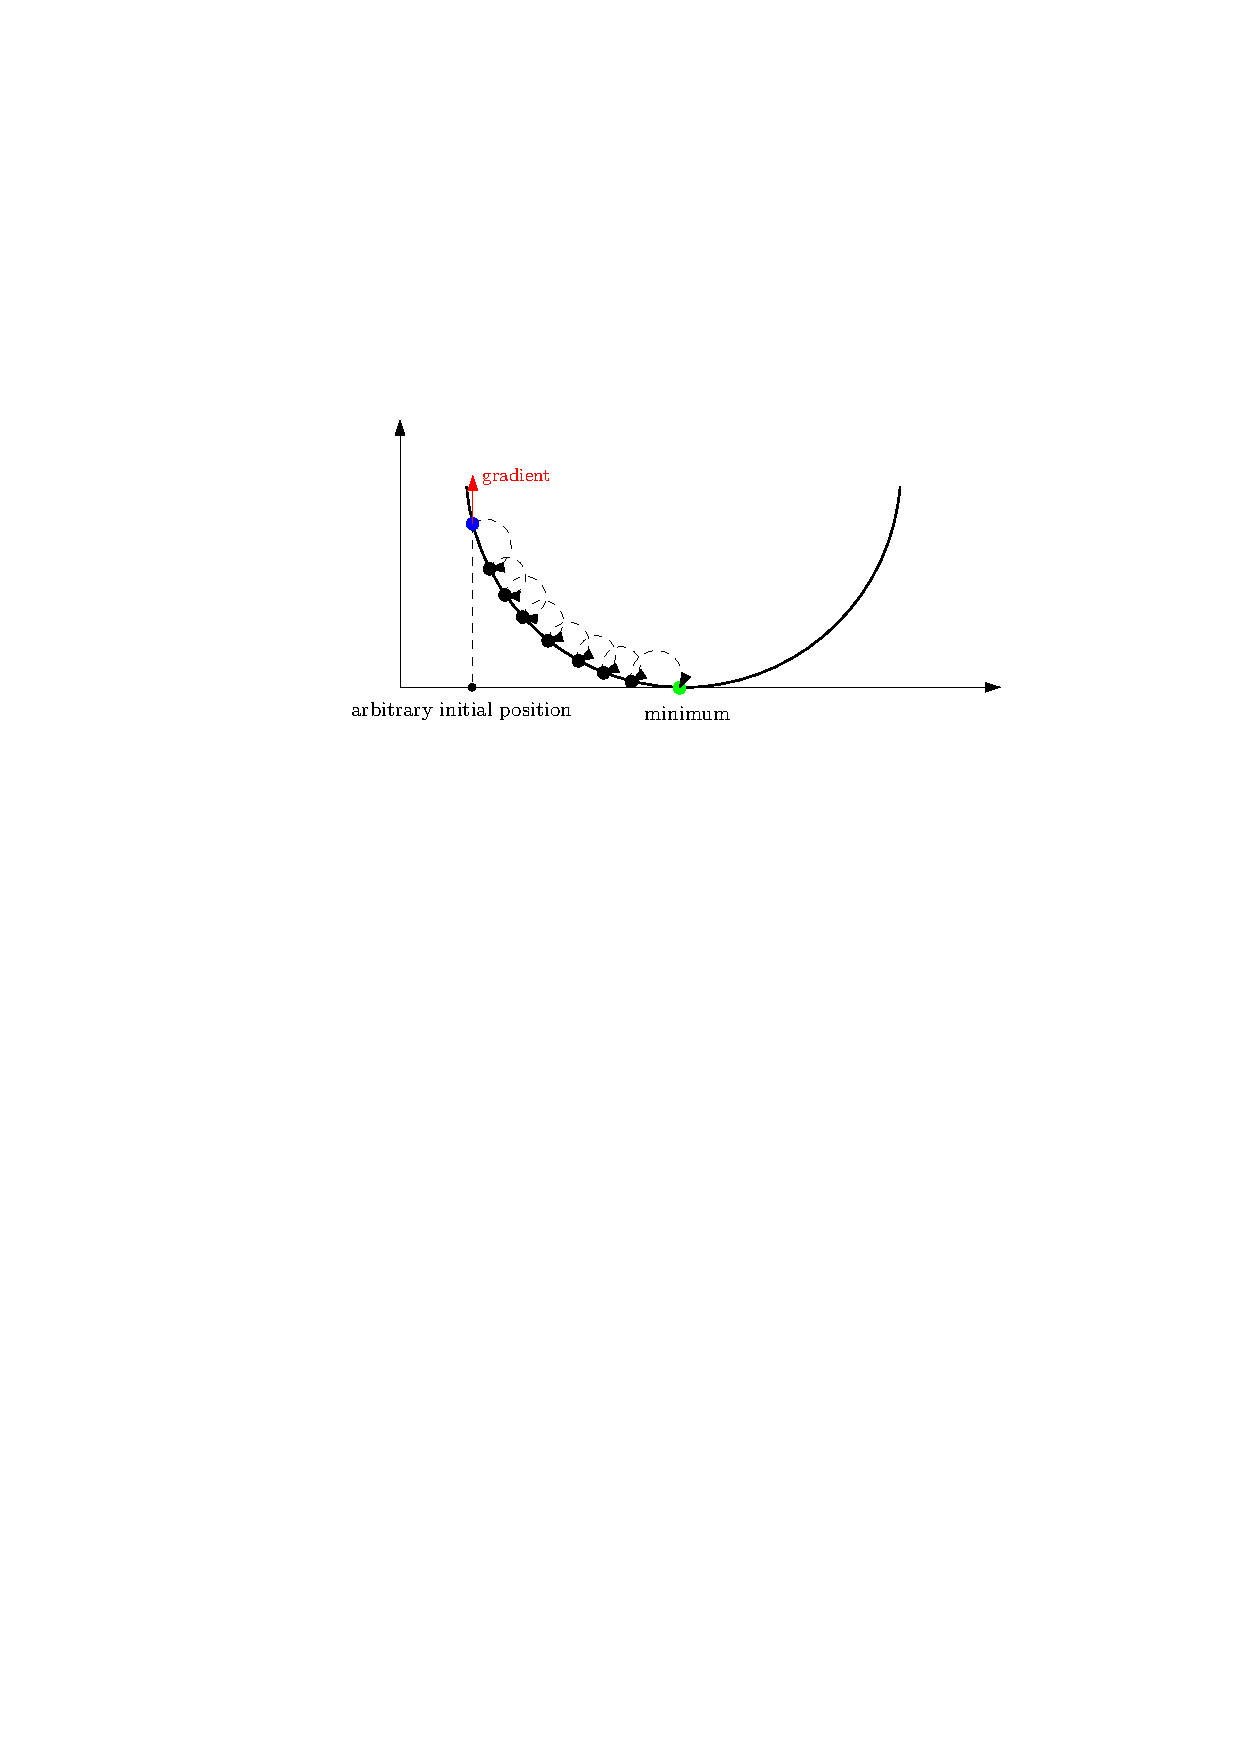
\includegraphics{theory/momentum.pdf}
        \caption{With momentum.}
        \label{fig:theory_momentum}
    \end{subfigure}
    \caption{Illustrative examples of gradient descent trajectories with and without momentum.}
    \label{fig:momentums}
\end{figure}

So, the position $g_i$ at iteration $i$ of a guard $g$ is not calculated anymore based only on the current computation of gradient descent. Instead, it also takes into account past values of gradient descent. In order to decide how much past states influence the value of the current position, we  take each gradient value with a weight.

Let $M_i(g_i)$ be the momentum for a guard at iteration $i$. Let $\bigtriangledown f_i(g_i)$ be the computation of the gradient descent in iteration $i$. Let the weight of a gradient descent value be a hyperparameter $\gamma$. 
As such, we  take into account the value of the previous gradient $\bigtriangledown f_{i - 1}(g_{i - 1})$ with weight $\gamma$. However, we still want the current gradient $\bigtriangledown f_i(g_i)$ to influence the guard's movement. This can happen with a weight of $1 - \gamma$. So, the computation for the momentum at iteration $i$ becomes $$M_i(g_i) = \gamma M_{i - 1}(g_{i - 1}) + (1 - \gamma)\bigtriangledown f_i(g_i).$$

We start with $$M_0(g_0) = (1 - \gamma) \bigtriangledown f_0(g_0).$$
We  then check for correctness how  the next iterations of the momentum are carried out:
\begin{align*}
    % M_1 &= \gamma M_0 + (1 - \gamma) \Delta f_1 \\
    %     &= \gamma (1 - \gamma) \Delta f_0 + (1 - \gamma) \Delta f_1 \\
    %     &= (1 - \gamma) (\gamma \Delta f_0 + \Delta f_1) \\
    % M_2 &= \gamma M_1 + (1 - \gamma) \Delta f_2 \\
    %     &= \gamma (1 - \gamma) (\gamma \Delta f_0 + \Delta f_1) + (1 - \gamma) \Delta f_2 \\
    %     &= (1 - \gamma) (\gamma^2 \Delta f_0 + \gamma \Delta f_1 + \Delta f_2) \\
    % ... \\
    M_i(g) &= \gamma M_{i - 1}(g_{i - 1}) + (1 - \gamma) \bigtriangledown f_i(g_i) \\
        &= \gamma (\gamma M_{i - 2}(g_{i - 2}) + (1 - \gamma) \bigtriangledown f_{i - 1}(g_{i - 1})) + (1 - \gamma \bigtriangledown f_i(g_i)) \\ 
        &= \gamma^2 M_{i - 2}(g_{i - 2}) + (1 - \gamma)(\gamma \bigtriangledown f_{i - 1}(g_{i - 1}) + \bigtriangledown f_i(g_i)) \\
        &= \gamma^3 M_{i - 3}(g_{i - 3}) + (1 - \gamma)(\gamma^2 \bigtriangledown f_{i - 2}(g_{i - 2}) + \gamma \bigtriangledown f_{i - 1}(g_{i - 1}) + \bigtriangledown f_i(g_i)) \\
        &...
        % &= (1 - \gamma) (\gamma^i \Delta f_0 + \gamma^{i - 1} \Delta f_1 + ... + \gamma \Delta f_{i - 1} + \Delta f_i) \\
\end{align*}

In this way, our momentum computation exponentially decreases the influence of a past state over the guard's current movement. So, the previous value of the momentum  exerts its inertia with $\gamma$ influence over the new value of the momentum.

Similarly, the new position $g_i$ of guard $g$ with learning rate $\alpha$ is now calculated as $$g_i = g_{i - 1} + \alpha M_i(g_{i - 1}).$$

\newpage
\subsection{Reflex Vertex Pull}

This section presents an additional idea to our gradient descent algorithm: pulling a guard towards reflex vertices. The pull strategy makes use of the second derivative of our optimisation function $f(g) = \text{Area}(g)$.

% The first derivative primarily tells us about the direction the function is going. That is, it tells us if the function is increasing or decreasing.

% the second derivative tells us what the rate of change of a quantity is

As mentioned previously, we are using the first derivative to compute the gradient of a guard's movement. That is, we use the first derivative of $f(g)$ to find the direction of a guard's movement that increases its seen area. Additionally, we  also make use of the second derivative of $f(g)$ to explore what the rate of change in the area increase is. 

We can achieve a more rapid increase in the seen area if we move a guard closer to a reflex vertex. The closer a guard is moved to a reflex vertex, the larger the increase in the area seen past the vertex. If a guard is moved directly on a reflex vertex, then the area seen past the vertex is maximised. 

% An example of the latter case is displayed in Figure \ref{fig:top_reflex_vertex}. There, the guard $g$ has been moved on top of reflex vertex $r$ such that it can see the whole area behind it.

% \begin{figure}[h!]
%     \centering
%     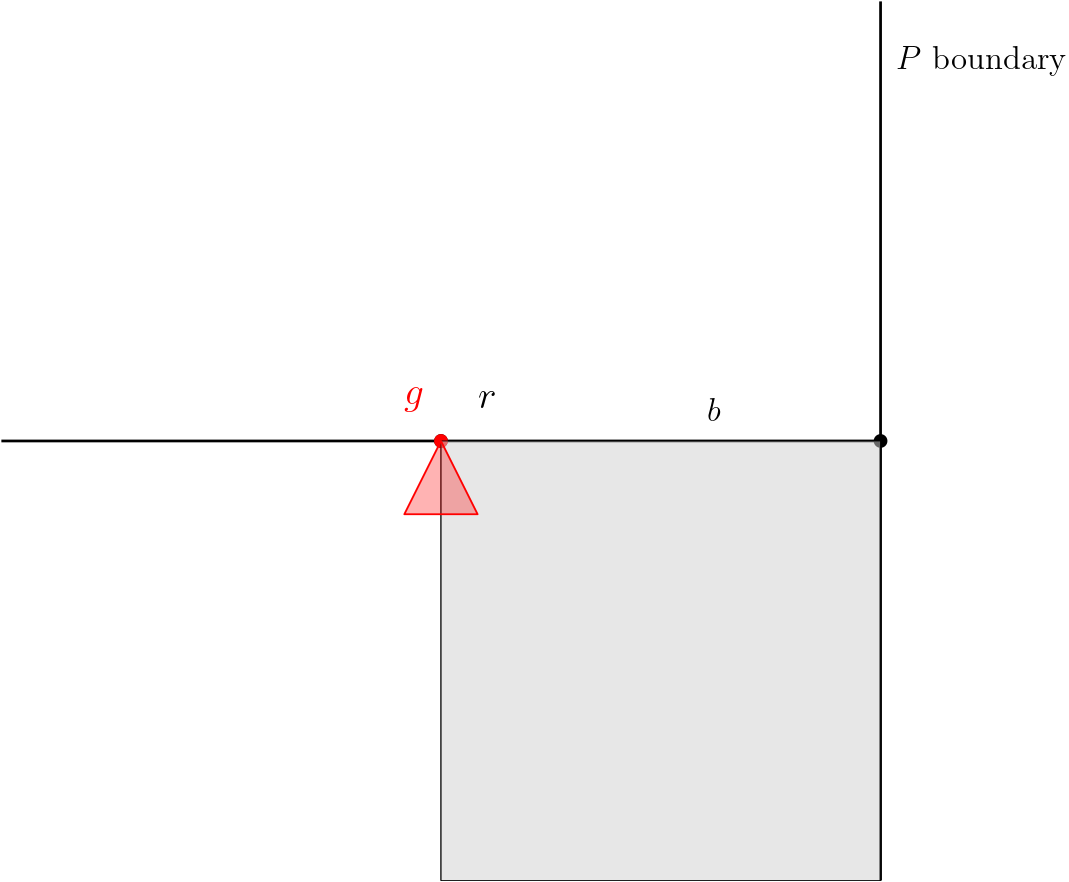
\includegraphics[width = 0.5\textwidth]{theory/pull2.png}
%     \caption{Guard placed on top of a reflex vertex can now see the whole area behind the reflex vertex.}
%     \label{fig:top_reflex_vertex}
% \end{figure}

We explore how the pull towards a reflex vertex $r$ can be computed, with an example in Figure \ref{fig:pull}. Let the guard $g = (0, 0)$, the reflex vertex $r = (2, 0)$ and the polygon boundary intersection point be $(5, 0)$. So, the distances $a = 2$ and $b = 3$ are known. Let $h_r$ be the pull in question. Let $g'_y$ be the new coordinates of guard $g$ when only the gradient is taken into account. In that case, we are only interested in the small movement $\partial y$. Analogously, let $g'_x$ be the new coordinate of guard $g$ when $g$ moves by a small amount $\partial x$ towards the reflex vertex. As previously, and without losing generality, assume that $g$ and $r$ have the same $x$-coordinate by rotating the plane $R$. Combining the two movements together results in $g'$ being the final position of $g$.

\begin{figure*}[!h]
    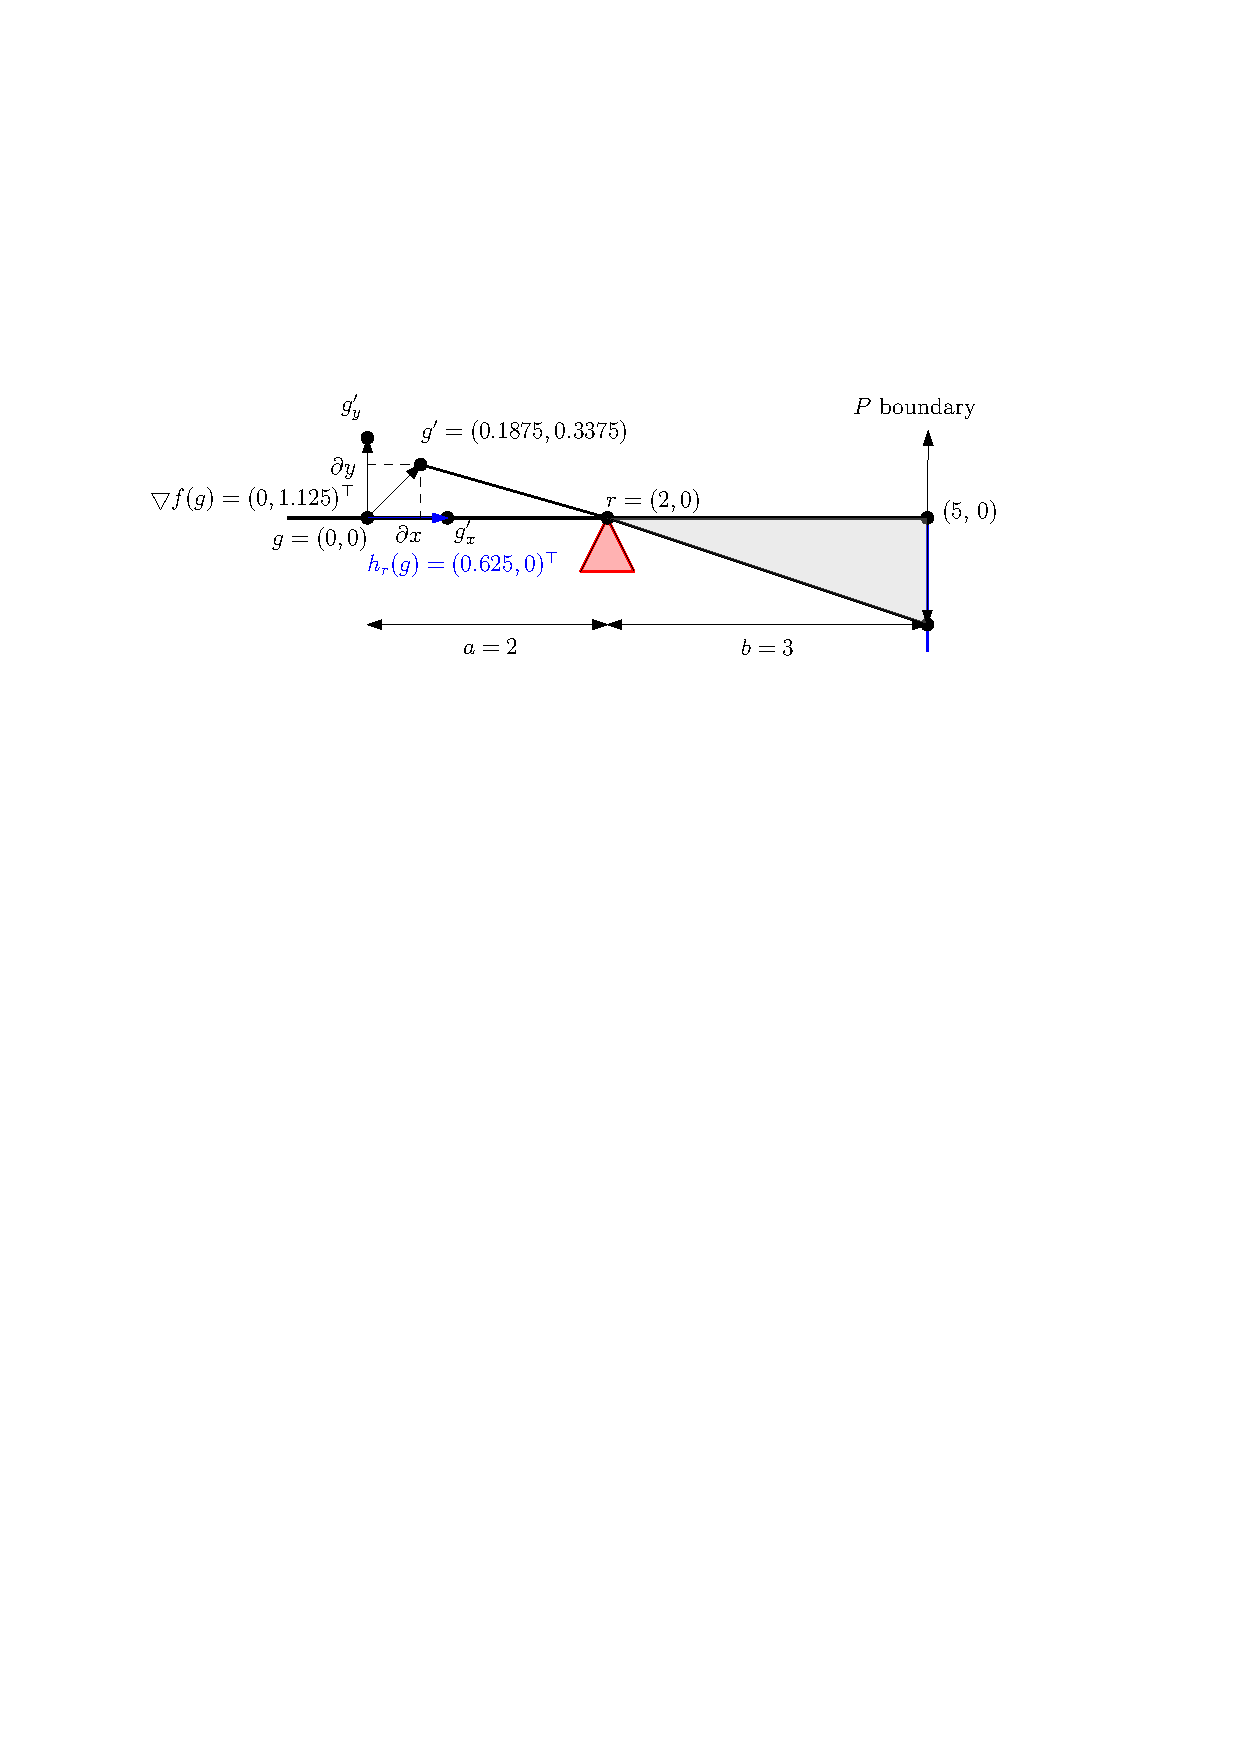
\includegraphics{theory/pull.pdf}
    \centering
    \caption{Computing the movements of the guard $g$ based on both the gradient and the pull towards reflex vertex $r$. The new position of the guard with learning rate $\alpha = 0.3$ becomes $g' = (0.1875, 0.3375)$.}
    \label{fig:pull}
\end{figure*}

The gradient is computed as
$$\bigtriangledown f(g) \overset{(\ref{eq:f})}{=} (0, \frac{b^2}{2a^2})^\intercal = (0, \frac{9}{8})^\intercal = (0, 1.125)^\intercal.$$ 
The pull is computed as 
$$h_r(g) \overset{(\ref{eq:h})}{=} (\frac{b^2}{2a^3}, 0)^\intercal = (\frac{9}{16}, 0)^\intercal = (0.625, 0)^\intercal.$$
So, the new position $g'$ of the guard $g$ given the learning rate $\alpha = 0.3$ becomes 
$$g' = g + \alpha(\bigtriangledown f(g) + h(g)) = 0.3 ((0, 1.125)^\intercal + (0.625, 0)^\intercal) = (0.1875, 0.3375).$$

We explain how we arrived at the pull computation. The pull is the second derivative of the norm of the gradient, so 
$$h_r(g) = \bigtriangledown ||\bigtriangledown f_r(g)|| = \left(\frac{\partial \bigtriangledown f(g)}{\partial x}, \frac{\partial \bigtriangledown f(g)}{\partial y}\right)^\intercal = \left(\frac{\partial \bigtriangledown f(g)}{\partial x}, 0\right)^\intercal.$$  
We calculate $h_r$ as follows: the Euclidean norm of the gradient is $||\bigtriangledown f(g)|| = \frac{b^2}{2a} (\ref{eq:normf})$, so the norm of the second gradient is 
\begin{align*}
||h_r(g)||&= ||\bigtriangledown ||\bigtriangledown f(g)|||| \\
       &= ||\bigtriangledown (\frac{b^2}{2a})|| \\
       &= \frac{b^2}{2a}\frac{d}{da} \\
       &= b^2\frac{1}{2a}\frac{d}{da} \\
||h_r(g)||&= -b^2\frac{1}{2a^2}.
\end{align*}

Note that we are using the norm approximation heuristic 
\begin{align*}
    \bigtriangledown ||\bigtriangledown f(g)|| \approx \bigtriangledown &\sum_{i \in R(g)} ||f_i(g)||, \\
    &R(g) = \{\text{reflex vertices of } P \text{ seen by } g\}. 
\end{align*}
The reason for this choice is that computing the norm of the partial gradients, summing them and then computing their gradient is much easier than computing the gradient of their sum 
\begin{align*}
    \bigtriangledown ||\bigtriangledown f|| = \bigtriangledown ||&\sum_{i \in R(g)} f_i||, \\
    &R(g) = \{\text{reflex vertices of } P \text{ seen by } g\}.
\end{align*}
We are aware of the fallacies of this approximation. Take the opposing unit vectors $a_1 = (1, 0)^\intercal,$ $a_2~=~(-1, 0)^\intercal$. The sum of their norms $\sum_i ||a_i|| = 2$, whereas the norm of their sum is $||\sum_i a_i|| = 0$. Clearly, they are not the same. Nonetheless, we still consider this approximation due to computation speed improvements and easiness of use.

The pull $h_r(g)$ is directed towards the reflex vertex $r$. So, it has the same orientation as vector $\vec{v} = (r - g)$. We  normalise $h_r(g)$ with the norm of vector $\vec{v}$. Its norm is $||\vec{v}|| = \frac 1 a$. So, 
\begin{align}
    h_r(g) = \vec{v}\frac{-b^2}{2a^2}\frac 1 a = \vec{v}\frac{-b^2}{2a^3}. \label{eq:h}
\end{align}

Let $h(g)$ be the total pull for guard $g$. As for the gradient, the total pull for guard $g$ and all reflex vertices $r$ the guard sees is 
\begin{align*}
    h(g) = &\sum_{r \in R(g)} h_r(g), \\
    &R(g) = \{\text{reflex vertices of $P$ seen by $g$\}}.
\end{align*}

Therefore, the movement of a guard $g$ to the new position $g'$ takes both the gradient and the pull into account: $$g' = g + \alpha (\bigtriangledown f(g) + h(g)).$$ Additionally, we  choose how much influence the pull itself has in the movement of the guard by adding a hyperparameter $\beta$: $$g' = g + \alpha (\bigtriangledown f(g) + \beta h(g)).$$

\subsubsection{Pull onto the Reflex Vertex}
\label{sec:pull_onto}
We have now created a heuristic for pulling a guard closer to a reflex vertex based on the increase in the seen area behind the reflex vertex. It could happen however that the pull towards the reflex vertex is forceful. In this case, the guard could be moved past the reflex vertex, in between the reflex vertex and the polygon boundary. Although the area seen behind the reflex vertex would be maximised, the guard would ``unsee'' (parts of) the area seen from its initial position $g$. In order to address this particular edge-case, the guard is placed on the reflex vertex when the pull is strong enough. 

This section thus expands on a procedure that decides when a guard is best placed on a reflex vertex based on its pull towards it.

Firstly, we must define the condition of what a ``strong enough'' pull means. Such a pull would move the guard $g$ ``close enough'' to the reflex vertex. Hence, we need to define what a minimum the distance between the new guard position $g'$ and reflex vertex $r$ would be. The most straight-forward way to do so would be to assign a hyperparameter to the distance between $g$ and $r$. Recall that $||\overline{gr}|| = a$. For now, let $\frac 2 3$ be the factor of closeness of $g'$ to $r$. This means, that when the guard is more than two thirds of the distance close to the reflex vertex, then the guard is moved onto the reflex vertex: 
\begin{align}
    ||h_r(g)|| > \frac 2 3 a. \label{eq:h_a}
\end{align}

Next, we need to account for the case where the guard is close to multiple reflex vertices. Namely, we consider the specific edge-case when a guard is in between two reflex vertices, illustrated in Figure \ref{fig:pull_cancel}. Let $D$ be the minimum distance in between any two reflex vertices of polygon $P$:
\begin{align*}
    D = &\min_{q \neq r} \text{ distance}(q, r), \\
    &\forall q, r \in P \text{ reflex vertices}.
\end{align*}
Let $g$ be a guard in between two reflex vertices $r_1$ and $r_2$ at distance $D$ from each other. Let the pulls $h_{r_1}(g)$ and $h_{r_2}(g)$ be strong towards $r_1$ and $r_2$, respectively. However, because they are opposites in directions, they cancel each other out, resulting in $g$ possibly not changing its position at all.

\begin{figure}[h!]
    \centering
    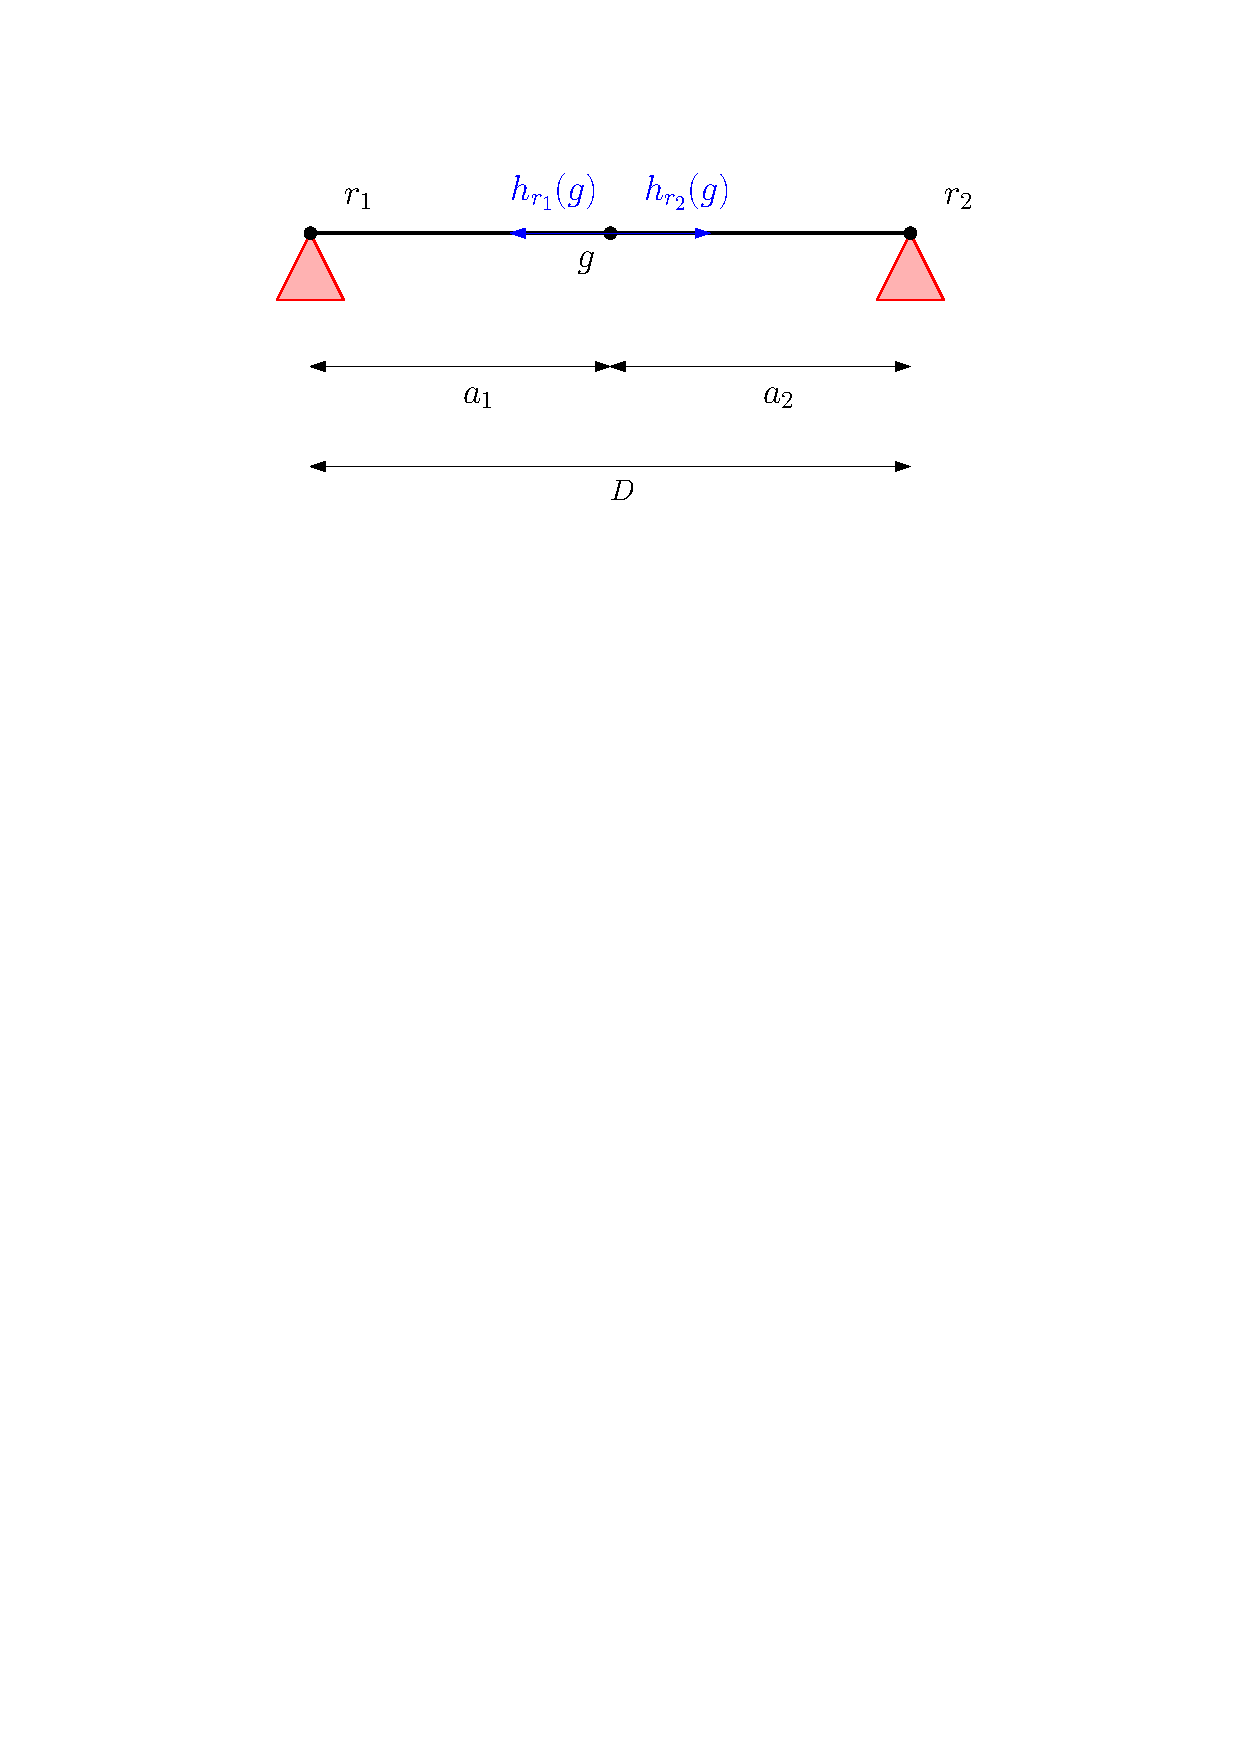
\includegraphics{theory/pull3.pdf}
    \caption{Guard $g$ is in between two reflex vertices $r_1$ and $r_2$. Because they are collinear, $g$ is equidistant from them and the pulls are equally strong $||h_{r_1}(g) = h_{r_2}(g)$, they cancel each other out.}
    \label{fig:pull_cancel}
\end{figure}

We  now introduce another condition for pulling the guard towards the closer reflex vertex when pulls are cancelling each other out. If a guard $g$ is not equidistantly placed in between two reflex vertices, we are interested in computing what the closer reflex vertex is. So, if $g$ is closer to a reflex vertex than half of the minimum distance in between any two reflex vertices $\frac D 2$, then we consider it close enough if: $$a < \frac D 2.$$
In this case we  choose to still move towards one of the reflex vertices and make progress.

An example of moving on top of a reflex vertex is found in Figure \ref{fig:pull_onto}. Let the guard $g = (1, 0)$, the reflex vertex $r = (2, 0)$ and the polygon boundary intersection point be $(5, 0)$. So, the distances $a = 1$ and $b = 3$ are known. Let $h_r(g)$ be the pull in question. The gradient is computed as
$$\bigtriangledown f(g) \overset{(\ref{eq:f})}{=} (0, \frac{b^2}{2a^2})^\intercal = (0, \frac{9}{2})^\intercal = (0, 4.5)^\intercal.$$
The pull is computed as 
$$h_r(g) \overset{(\ref{eq:h})}{=} (\frac{b^2}{2a^3}, 0)^\intercal = (\frac{9}{2}, 0)^\intercal = (4.5, 0)^\intercal.$$
The guard is close enough to $r$ to be moved onto it (\ref{eq:h_a}):
$$||h_r(g)|| > \frac 2 3 a \iff 4.5 > \frac 2 3.$$
So the new coordinate of the guard is $g' = r = (2, 0)$.
they
Note that Figure \ref{fig:pull_onto} displays how the closer the guard to a reflex vertex is, the stronger its pull. This comes in contrast with Figure \ref{fig:pull}. Given the same reflex vertex $r$ and polygon boundary coordinates, the guard $g = (0, 0)$ was farther away, and its pull $h_r(g) = (0.625, 0)^\intercal$ was thus not as strong. Hence, we only want to place guards on reflex vertices when their pull is strong enough.

\begin{figure}
    \centering
    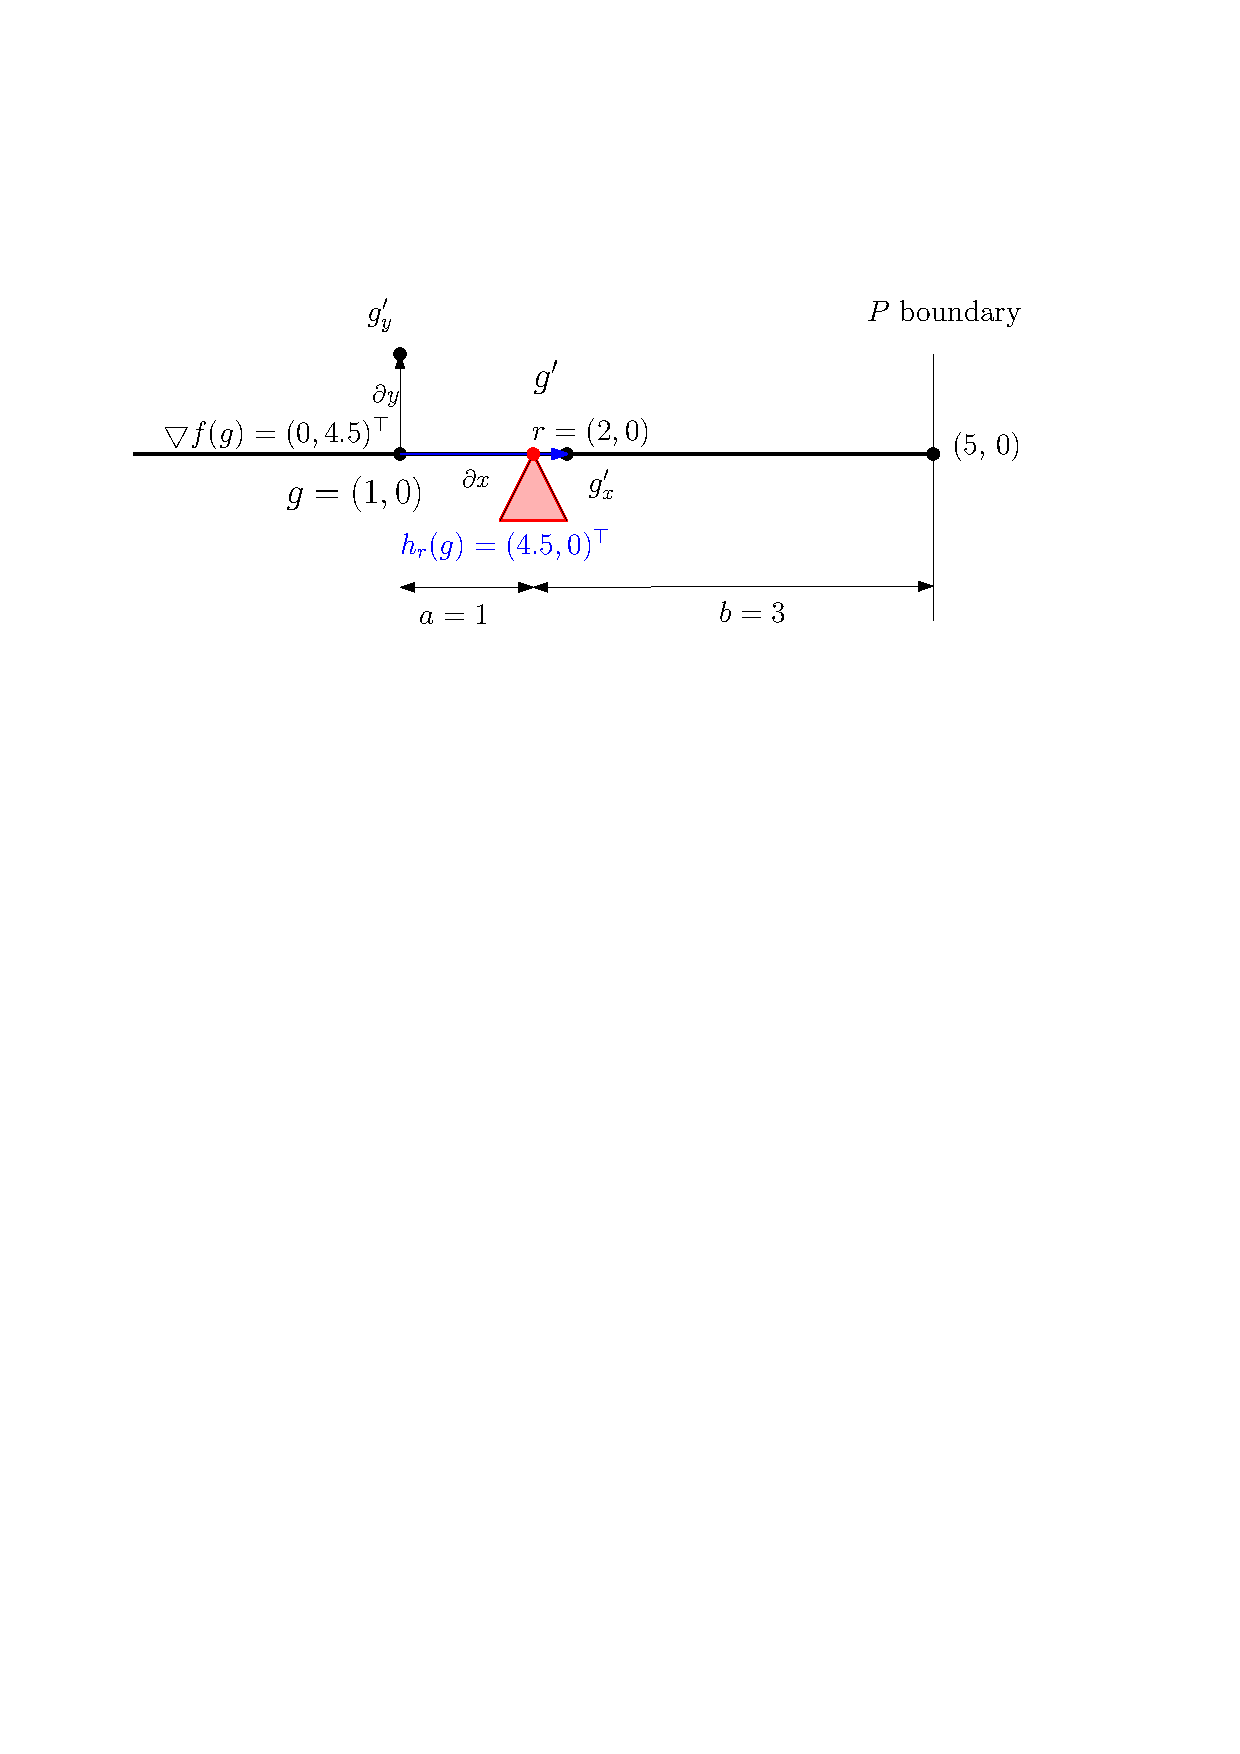
\includegraphics{theory/pull_onto.pdf}
    \caption{Computing the movements of the guard $g$ based on both the gradient and the pull towards reflex vertex $r$. The guard $g$ is close enough to $r$ (\ref{eq:h_a}), so $g$ is placed on top of the reflex vertex $r$.}
    \label{fig:pull_onto}
\end{figure}

\subsubsection{Pull Capping}
\label{sec:pull_capping}
Nonetheless, it can happen that the pull towards a reflex vertex is significantly larger in comparison to the gradient and the momentum. In that case, if the guard is not pulled onto the reflex vertex, it would at least have a huge jump towards the reflex vertex.

We want to smoothen out possibly erratic movement jumps. Just like in the case of momentum, we want our pull to be smoothened out when it is ``suddenly too large''. We define what ``suddenly too large'' is based on the momentum. If the pull is larger than a factor of $\mu$ than the momentum and a constant $c$, then we cap it at that value. So, at step $i$, the momentum $h_i(g_i)$ is capped as:
\begin{align*}
    \text{if } ||h_i(g_i)|| &> \mu ||M_i(g_i)|| + c \text{, then} \\
               h_i(g_i) &= h_i(g_i) \frac{\mu ||M_i(g_i)||}{||h_i(g_i)||}.
\end{align*}
The factor $\mu$ becomes thus a hyperparameter to experiment with.

% \newpage
\subsection{Reflex Area}
\label{sec:reflex_area}
% - address the issue of a guard "losing" the seen area gained after moving on top of a reflex vertex + its movement in and out of the reflex vertex
An additional heuristic is introduced in this section: the concept of \textit{reflex area}. The reflex area heuristic counteracts a specific edge-case: a guard placed on a reflex vertex would move behind the reflex vertex. As such, it would stop seeing the area that it was seeing before. We want to prevent this loss in area seen. So, we are restricting the movement of the guard away from the reflex vertex such that it continues seeing the same areas it was seeing from the reflex vertex.
% design choice was made to counter-act the edge-case of a guard moving away from a reflex vertex and ``unseeing'' the area that it was already seeing. 

This case is illustrated in Figure \ref{fig:pull_to_on_behind}. In Subfigure \ref{fig:pull_to_on_behind1}, guard $g$ starts moving with pull $h_r(g)$ towards reflex vertex $r$. The pull is strong enough to place $g$ on $r$ in Subfigure \ref{fig:pull_to_on_behind2}. In this case, $g$ sees everywhere around $r$. However, the new gradient $\bigtriangledown f(g)$ of $g$ moves it past $r$ in Subfigure \ref{fig:pull_to_on_behind3}. The initially seen area before $r$ is now not completely seen anymore by $g$.

Let $rr'$ and $rr''$ be the extensions to the polygon boundary segments whose intersection is the reflex vertex $r$. We call \textit{reflex area} the area between line segments $rr'$ and $rr''$ that is contained inside the polygon. Subfigure \ref{fig:reflex_area} draws the reflex area more closely. If a guard $g$ has to move outside the reflex area, we project its new position $g'$ onto the closest reflex line (in this case, $rr'$). Naturally, if $g$ has to move inside the reflex area, it can do so unaffectedly. In this way, we maintain the gained property of a guard seeing everything around a reflex vertex while still allowing it to move away from the reflex vertex.

\newpage
\begin{figure}[h!]
    \centering
    \begin{subfigure}{0.45\textwidth}
        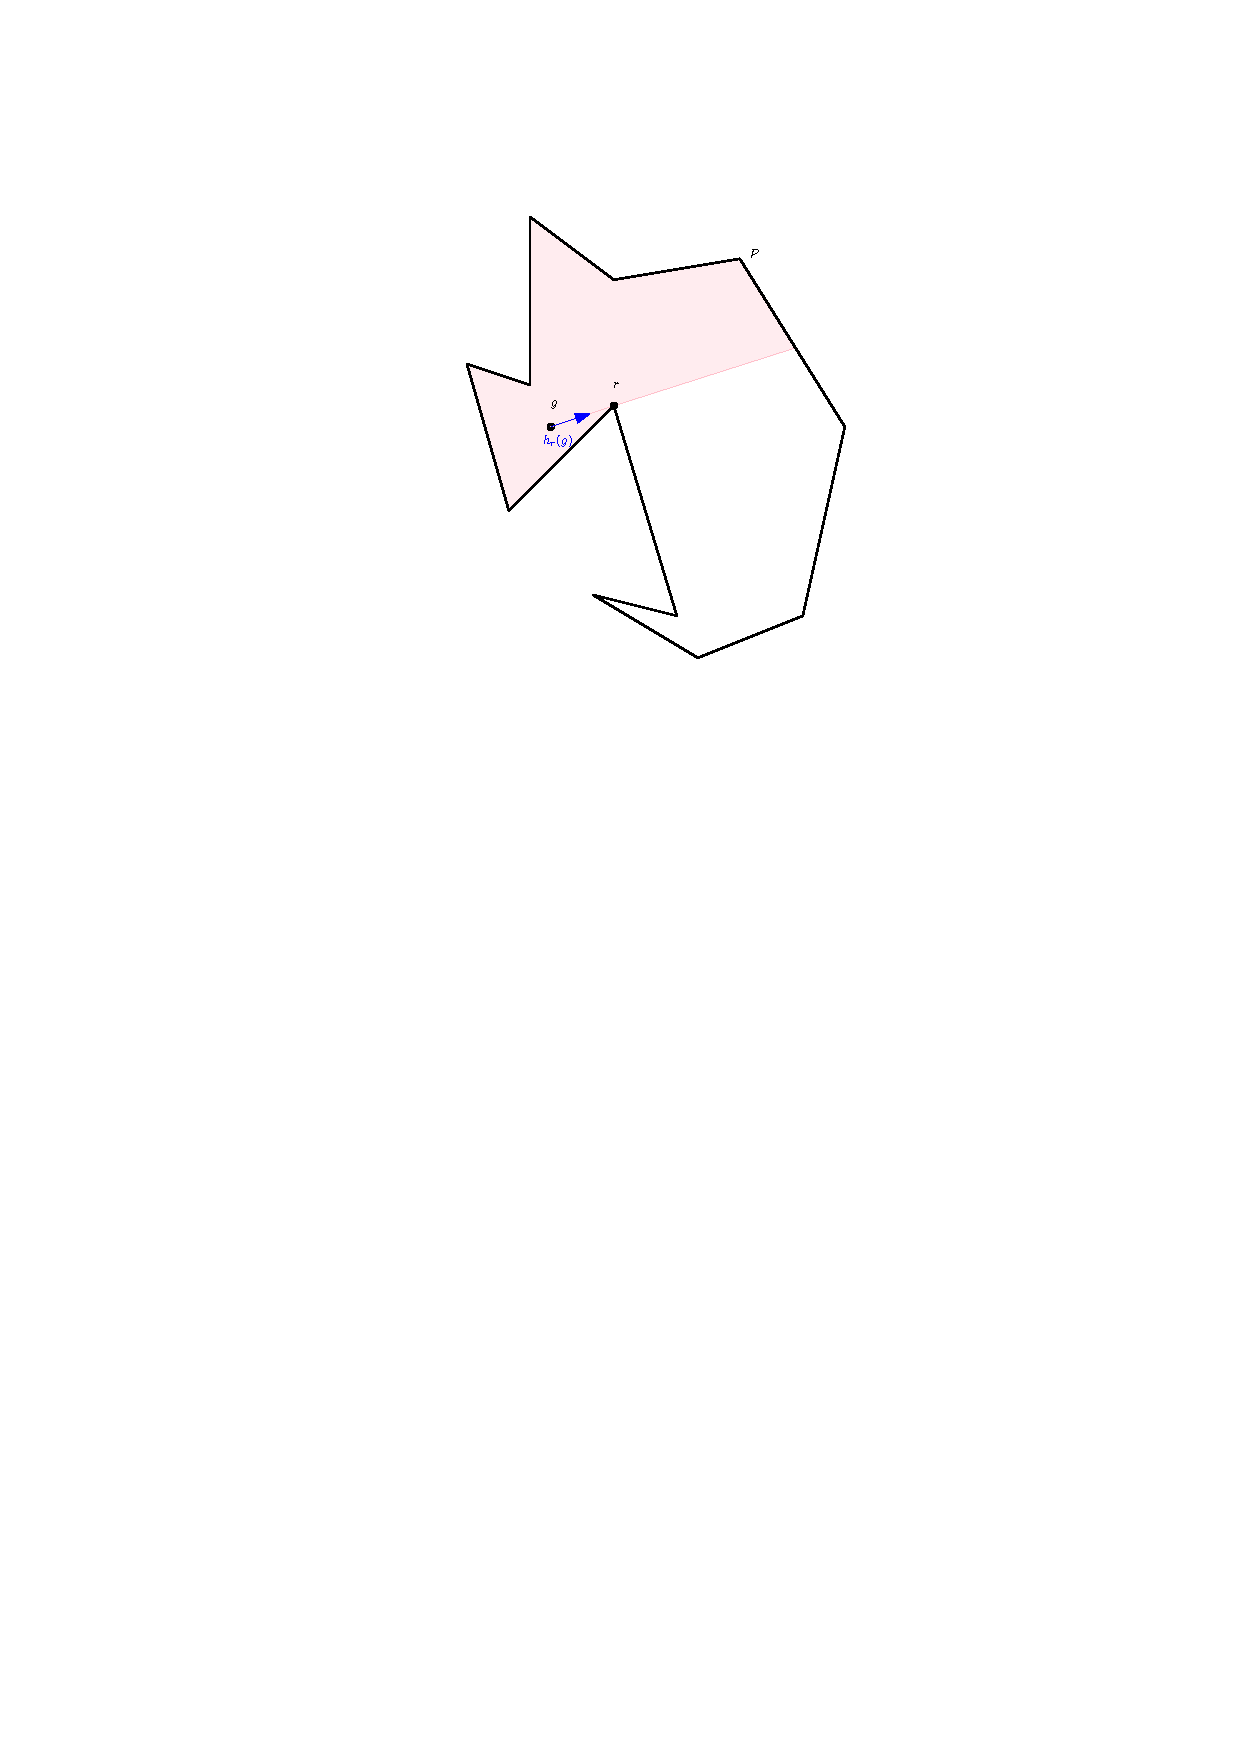
\includegraphics{theory/reflex_area_to_vertex.pdf}
        \caption{Guard $g$ starts moving with pull $h_r(g)$ towards reflex vertex $r$. Guard $g$ cannot see past $r$.}
        \label{fig:pull_to_on_behind1}
    \end{subfigure}
    \hfill
    \begin{subfigure}{0.45\textwidth}
        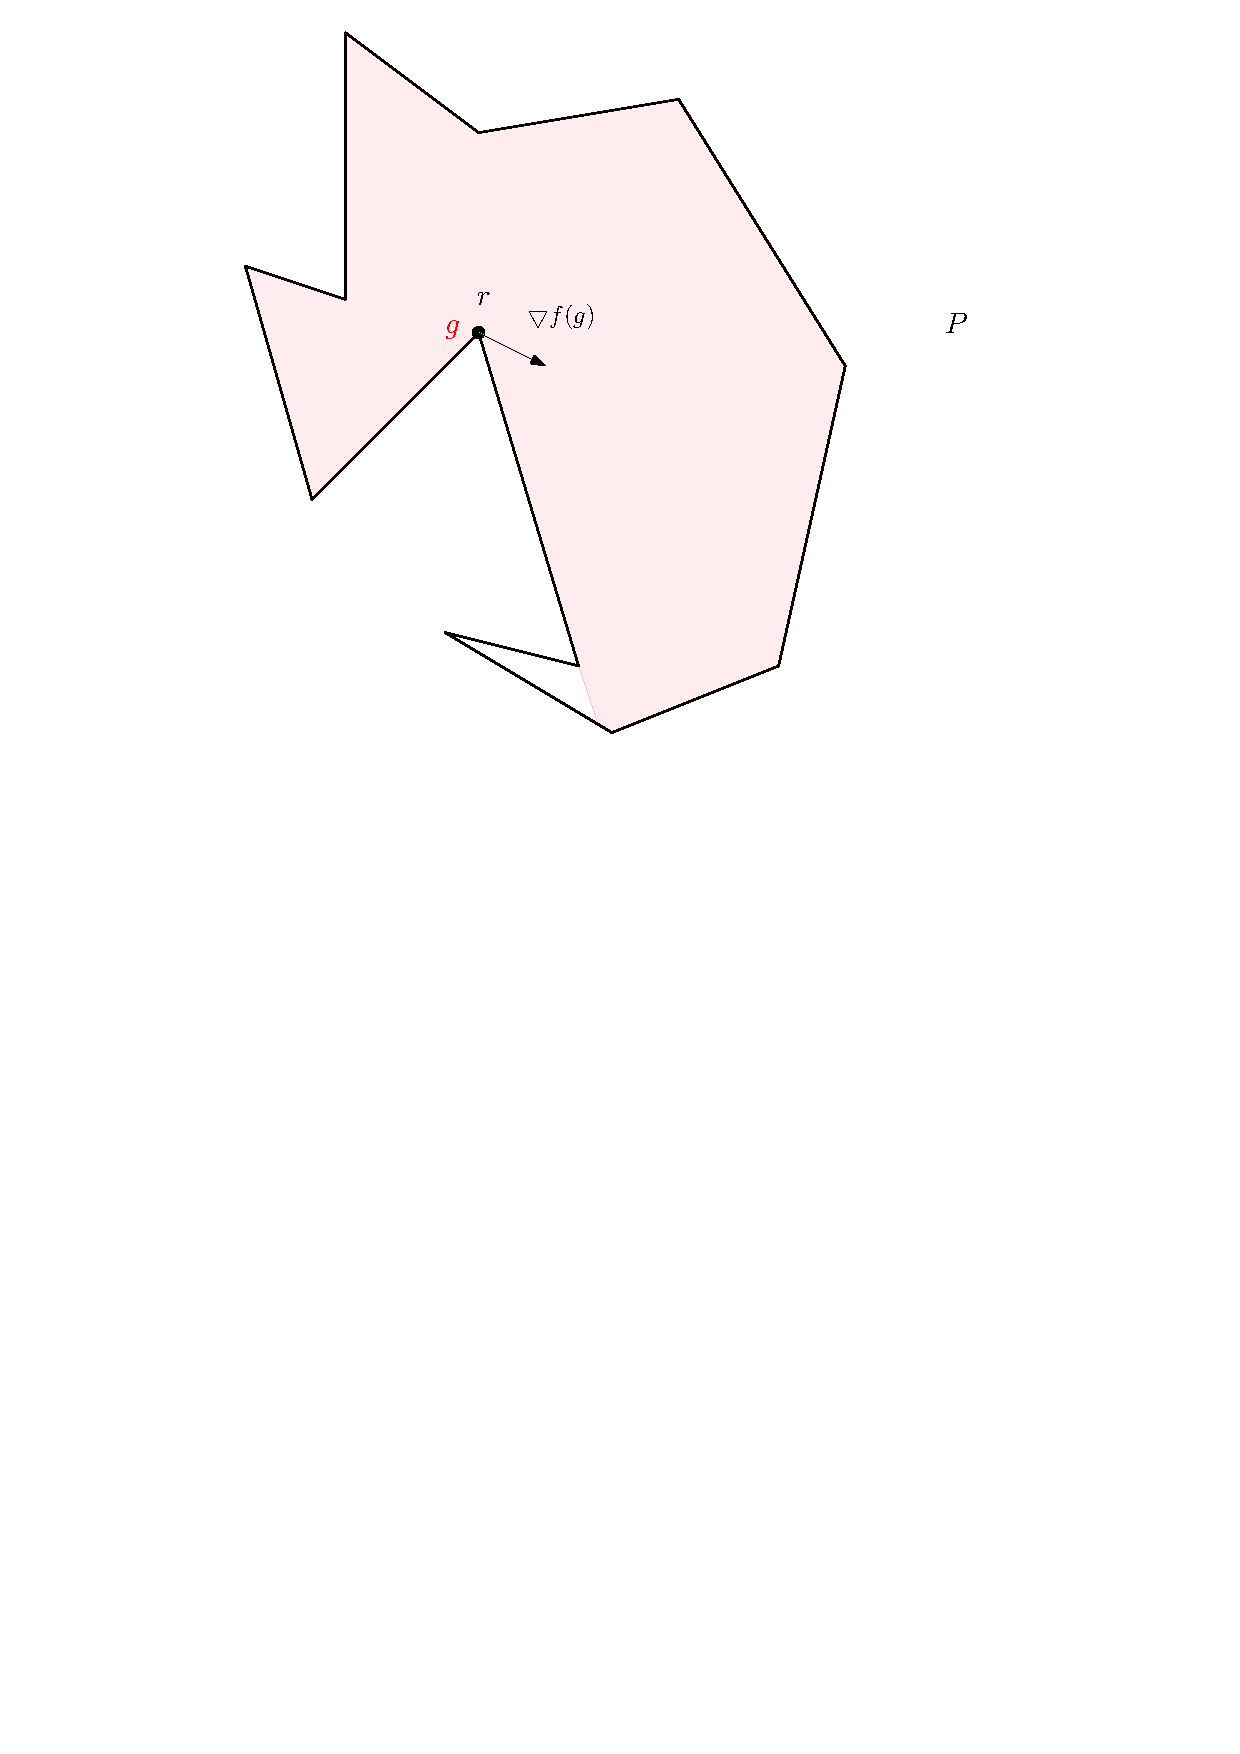
\includegraphics{theory/reflex_area_on_vertex.pdf}
        \caption{Guard $g$ is placed on reflex vertex $r$. Guard $g$ sees both before $r$ and past it.}
        \label{fig:pull_to_on_behind2}
    \end{subfigure}
    \begin{subfigure}{0.45\textwidth}
        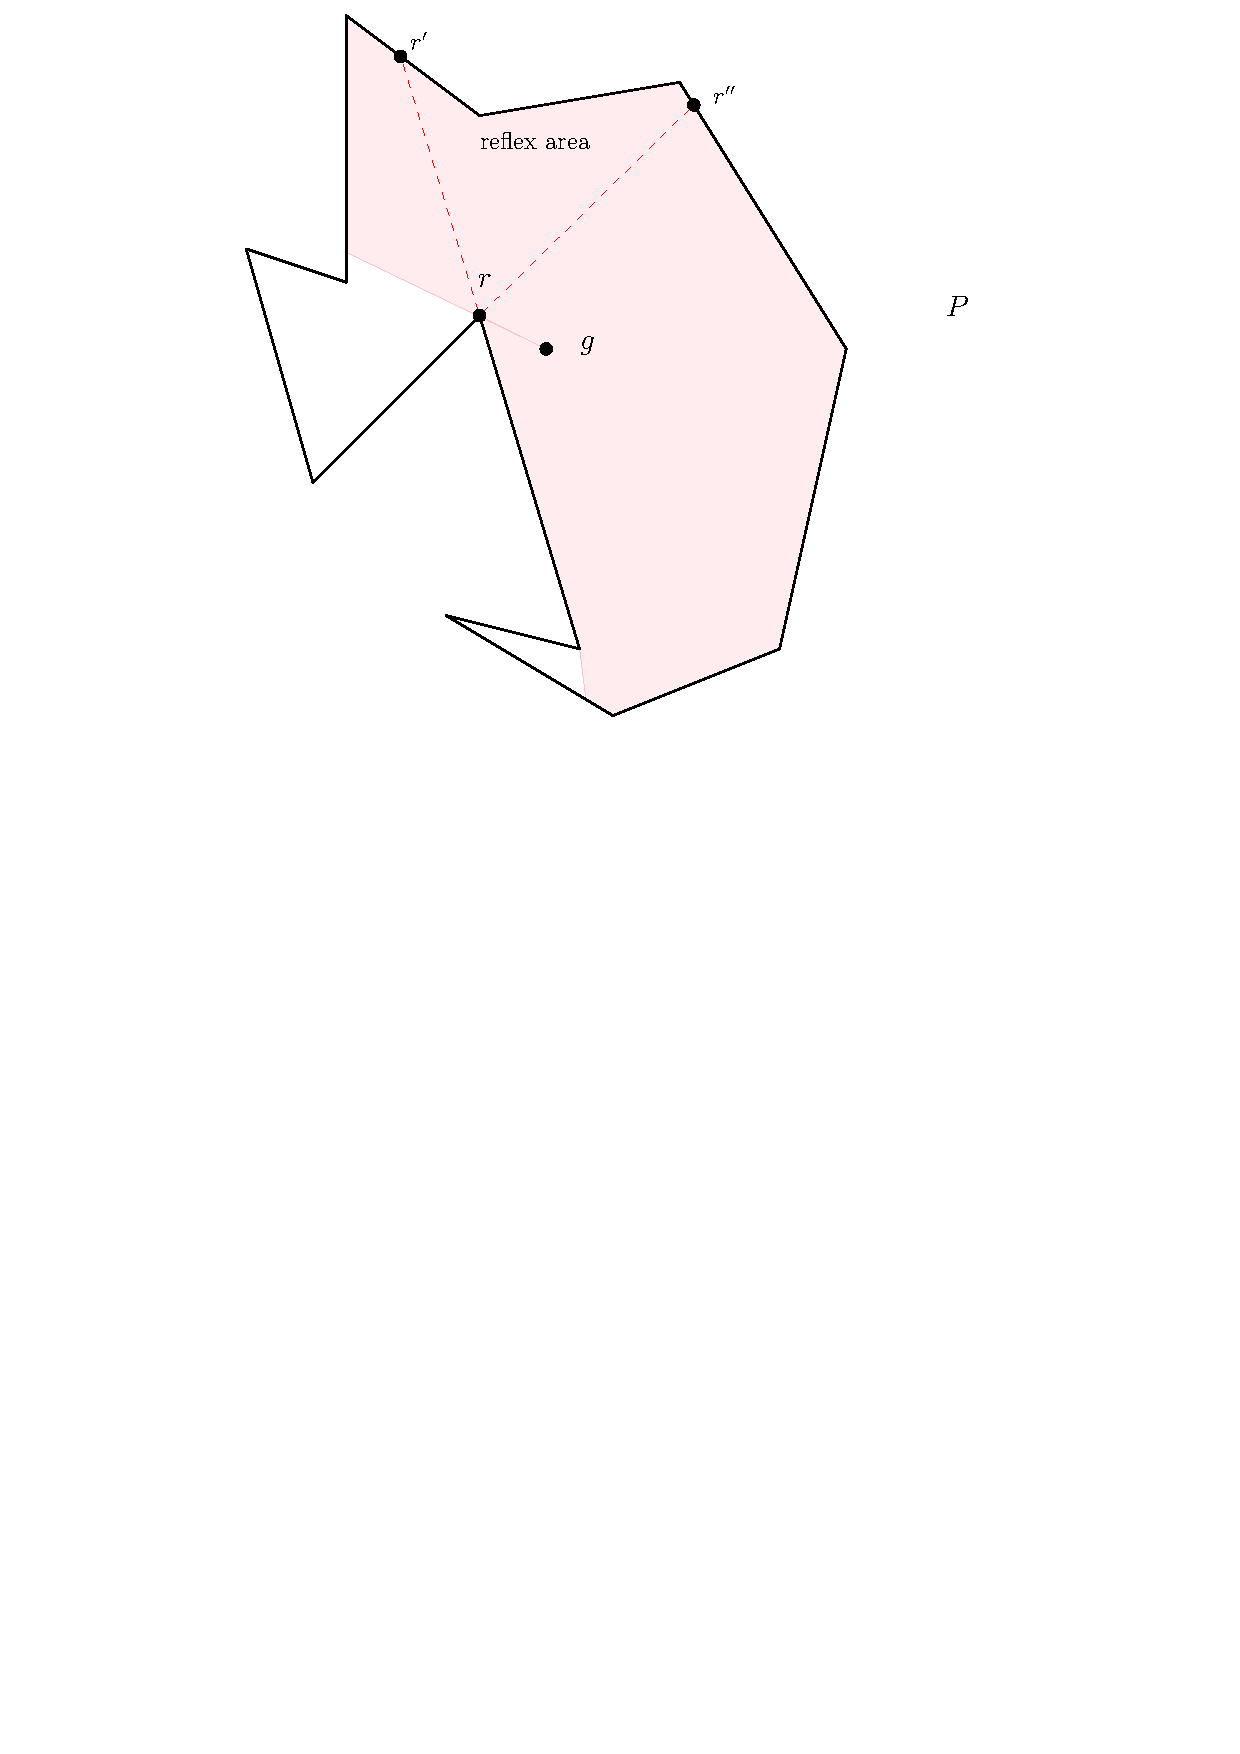
\includegraphics{theory/reflex_area_behind_vertex.pdf}
        \caption{Guard $g$ has moved past reflex vertex $r$. Guard $g$ cannot see anymore before $r$.}
        \label{fig:pull_to_on_behind3}
    \end{subfigure}
    \hfill
    \begin{subfigure}{0.45\textwidth}
        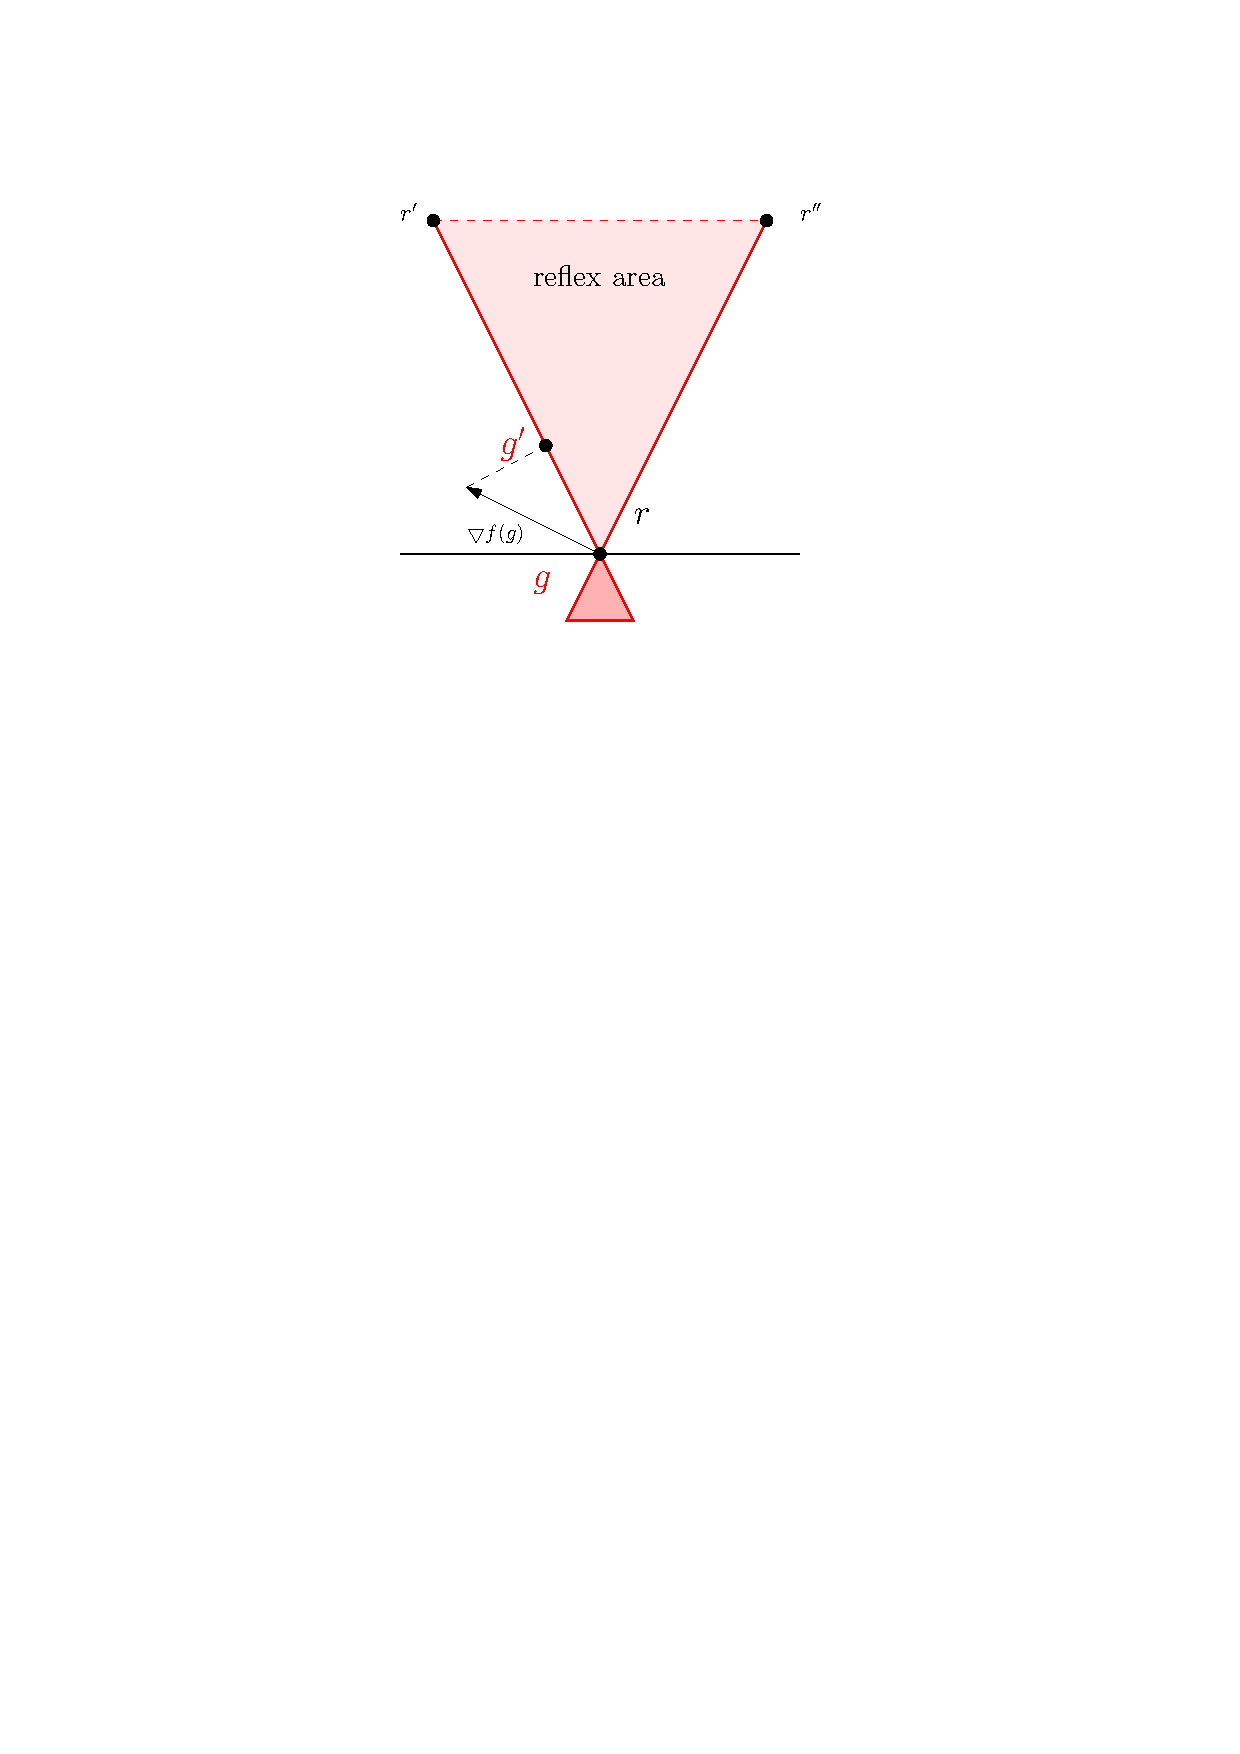
\includegraphics{theory/reflex_area.pdf}
        \caption{The movement of $g$ is restricted inside the reflex area.}
        \label{fig:reflex_area}
    \end{subfigure}
    \caption{Guard $g$ moves towards and on the reflex vertex $r$. Eventually, its newly computed position is away from $r$ and the reflex area. This results in $g$ not seeing the initial area anymore. So, its movement is restricted to the reflex area $\triangle rr'r''$. If $g$ needs to move outside the reflex area, its new position is projected on the closest reflex line.}
    \label{fig:pull_to_on_behind}
\end{figure}

\newpage
\subsection{Line Search}
\label{sec:line_search}
We introduce in this section another extension to the regular gradient descent algorithm: Line Search \cite{swann1969survey}. Given a step size, its aim is to search for the best solution on the gradient descent line. 

Figure \ref{fig:line} illustrates an example for this extension. Take guard $g$ and reflex vertex $r$. Let $\frac 1 x$ be the starting search factor, and $s$ the step size factor. Recall that $M_i(g)$ is the optimal movement direction for a guard at iteration $i$. As such, line search  computes the optimal guard position $g_{i + 1} = g_i + \frac{s^t}{x}M_i(g_i),$ with $t$ the best step power for the guard from $\{\frac{s^0}{xM_i}, \frac{s}{x}M_i(g_i), \frac{s^2}{x}M_i(g_i), ...\}$. The dashed line represents the direction of gradient descent, as computed based on the gradient and reflex vertex pull computations. Given a step size $s$, 3 different possible new guard positions are identified: $g'_{i_1} = g_i + \frac 1 xM_i(g_i)$,  $g'_{i_2} = g_i + \frac s x M_i(g_i)$, $g'_{i_3} = g_i + \frac{s^2}{x} M_i(g_i)$.
% By starting with a proper step size factor, we deploy a more finely-grated search closer to the actual value of the gradient. The proper step size factory checks thus whether the gradient descent overshoots. Then, we will check for the best solutions with an improper step size factor. This will allow us to search for a guard positioning farther than the gradient. Lastly, we will also check whether the actual gradient value is the best.
The optimal guard is the one who has the largest increase in the area seen. If the global area is not increased, a best solution is also chosen if a guard is gaining visibility to a previously unseen part of the polygon, regardless of the area increase.

It is worth mentioning that Line Search deems the use of a learning rate obsolete. Because the search factor finds the optimal position on the direction line, it acts thus as a learning rate.

\begin{figure}[h!]
    \centering
    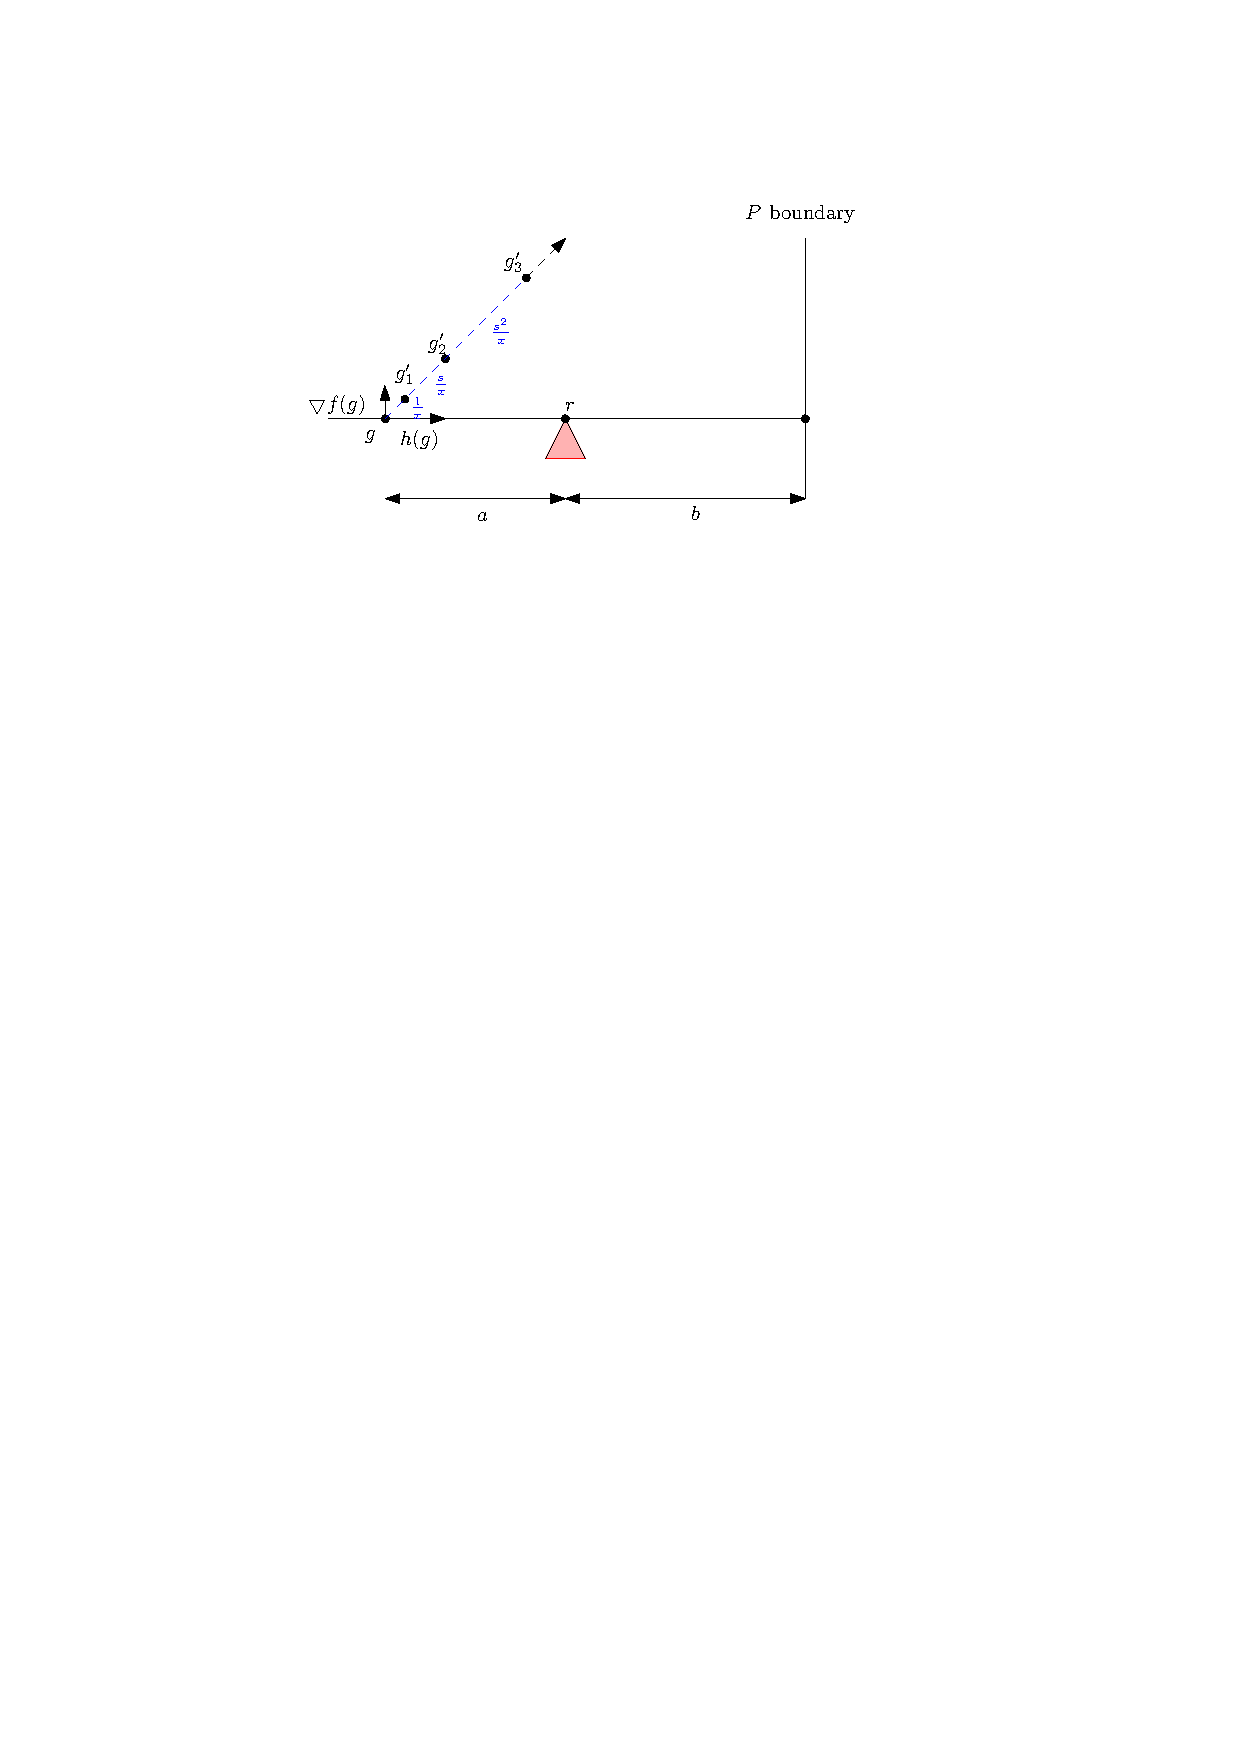
\includegraphics{theory/line_search.pdf}
    \caption{The gradient descent line gives the direction of searching for the optimal guard position. Given step sizes $\frac 1 x, \frac s x, \frac{s^2}{x}$, there are 3 possible guard positioning on the dashed gradient descent line: $g'_{i_1}, g'_{i_2}, g'_{i_3}$. The best of them is chosen based on the size of the newly visible area seen.}
    \label{fig:line}
\end{figure}


\subsection{Angle Behind Reflex Vertex}
\label{sec:angle}
% - take into consideration how much a guard should move towards a reflex vertex, depending on the area seen behind it
We propose in this section a heuristic that further fine-tunes the factor with which a guard's movement is influenced by a reflex vertex. Currently, we only take into account the distance $b$ between the reflex vertex and the polygon boundary. Intuitively, the unseen area behind the reflex vertex should also play a role in the computation of the gradient: guards should be drawn faster to larger areas. In order to do so, we  take into account the normalised value of angle $\theta$ behind the reflex vertex.

A visualisation for this heuristic is found in Figure \ref{fig:angle}. The pull of the guard $g$ towards the reflex vertex $r$ is influenced by the normalised value of $\theta$ as follows: $$g' = g + (\frac{\theta}{2\pi} + c)(\bigtriangledown f(g) + \beta h(g)).$$

We  additionally add a constant $c$ to account for small angles. For example, if the normalised value of $\theta$ is close to $10^{-5}$, then $c = 10^{-2}$. Then the guard still has a significant move towards the unseen area, no matter how small it is. In this way, smaller areas are not overlooked.

\begin{figure}[h!]
    \centering
    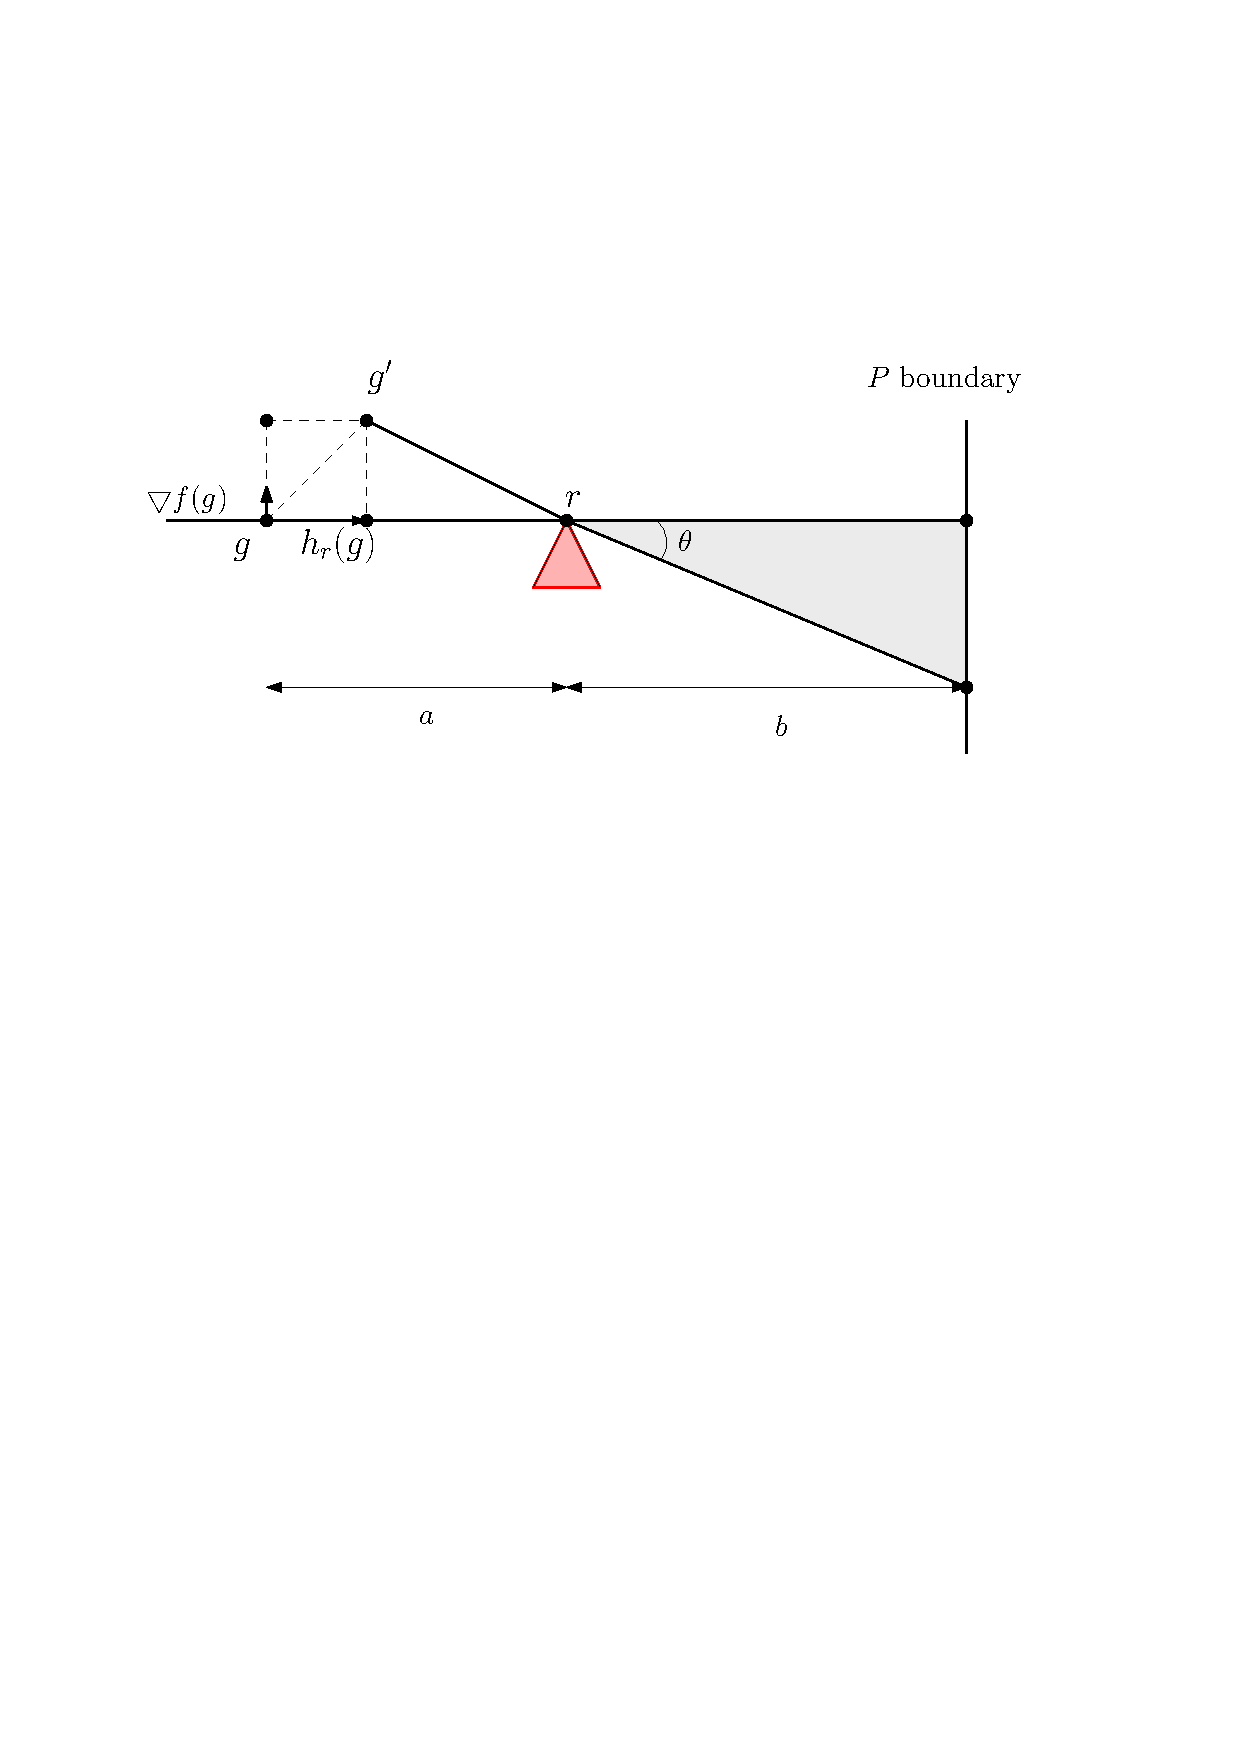
\includegraphics{theory/angle.pdf}
    \caption{The normalised angle $\mu$ behind the reflex vertex $r$ takes into account the factor with which the guard $g$ is drawn to $r$.}
    \label{fig:angle}
\end{figure}

\subsection{Hidden Movement}
\label{sec:hidden_gradient}
% - speed up the guard movement by giving all guards a gradient
This section tackles a computation speed-up for the case in which guards have a movement vector of 0 (they don't move). This can happen when the area seen by a guard is already completely seen by other guards. We consider that having a movement vector of 0 is detrimental to the progress of the algorithm. Note that we call \textit{movement vector} the sum of all heuristics that apply to computing the new position of a guard. The reason behind this is that it is unlikely that a guard's optimal position has been found when its movement vector is 0. Hence, we would like every guard to move, no matter how little.

In order to allow guards to still move when their movement vector is 0, we deployed the \textit{hidden gradient} heuristic. This heuristic is based on the fact that we allow guards whose movement vector is 0 to still move with a newly computed ``hidden'' movement vector. So, if there are guards whose movement vector is 0, we  recompute their movement vector by not taking into account the area seen by the guards who have a non-zero movement vector.

An example of this approach is found in Figure \ref{fig:hidden_gradient}. Let $G = \{g_1, g_2, g_3\}$ be the complete set of guards. Initially in Subfigure \ref{fig:hidden_gradient1}, only $g_1$ has a non-zero movement vector. The visibility regions of $g_2$ and $g_3$ are overlapping with that of $g_1$, so their movement vectors are 0. Let $G_0 = \{g_1\}$ be the set of guards who at step 0 have a non-zero movement vector. In this case, only $g_1$
Then, Subfigure \ref{fig:hidden_gradient2} displays the remaining set $G \setminus G_0$ of guards with a zeroed movement vector. The visibility area of guard $g_1$ overlaps with $g_2$, so only guard $g_2$ has a non-zero movement vector. So, $g_2$ is part of the set $G_1 = \{g_2\}$ of guards who at step 1 have a non-zero movement vector.
Lastly, we  compute the non-zero movement vector for guard $g_3$ in Subfigure \ref{fig:hidden_gradient3}. The guard $g_3$ can now be part of the set $G_2 = \{g_3\}$ which contains the guards who at step 2 have a non-zero movement vector.
In Subfigure \ref{fig:hidden_gradient4} all the guards have been moved to their new positions $g'_1, g'_2, g'_3$, respectively. So the movement vectors have been computed as $G = G_0 \cup G_1 \cup G_2$, where $G_1$ and $G_2$ contain the guards with hidden movements.

\begin{figure}[h!]
    \centering
    \begin{subfigure}{0.45\textwidth}
        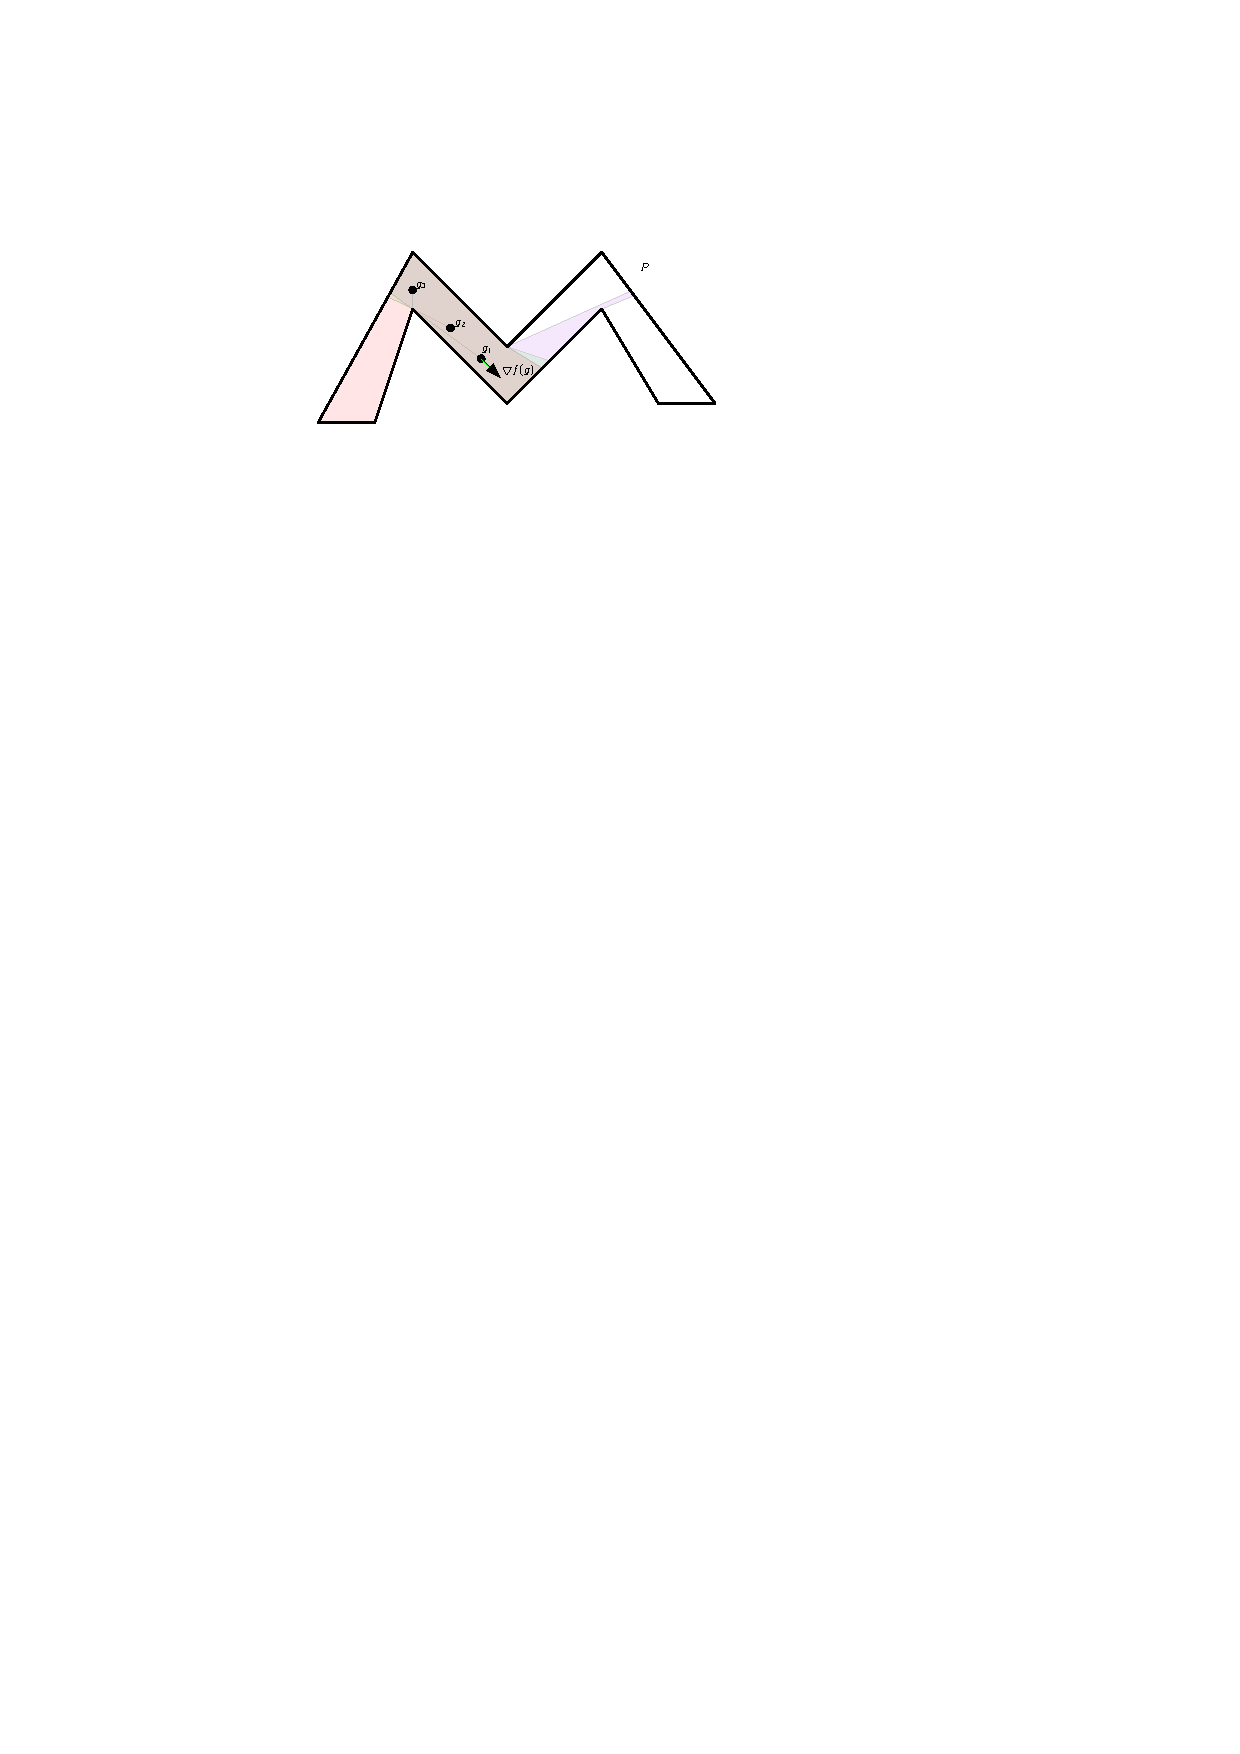
\includegraphics{theory/hidden_gradient1.pdf}
        \caption{Guard $g_2$ and $g_3$ have a movement vector of 0, because guard $g_1$ sees all the areas they see. So, the set of guards with a non-zero movement vector is $G_0 = \{g_1\}$.}
        \label{fig:hidden_gradient1}
    \end{subfigure}
    \hfill
    \begin{subfigure}{0.45\textwidth}
        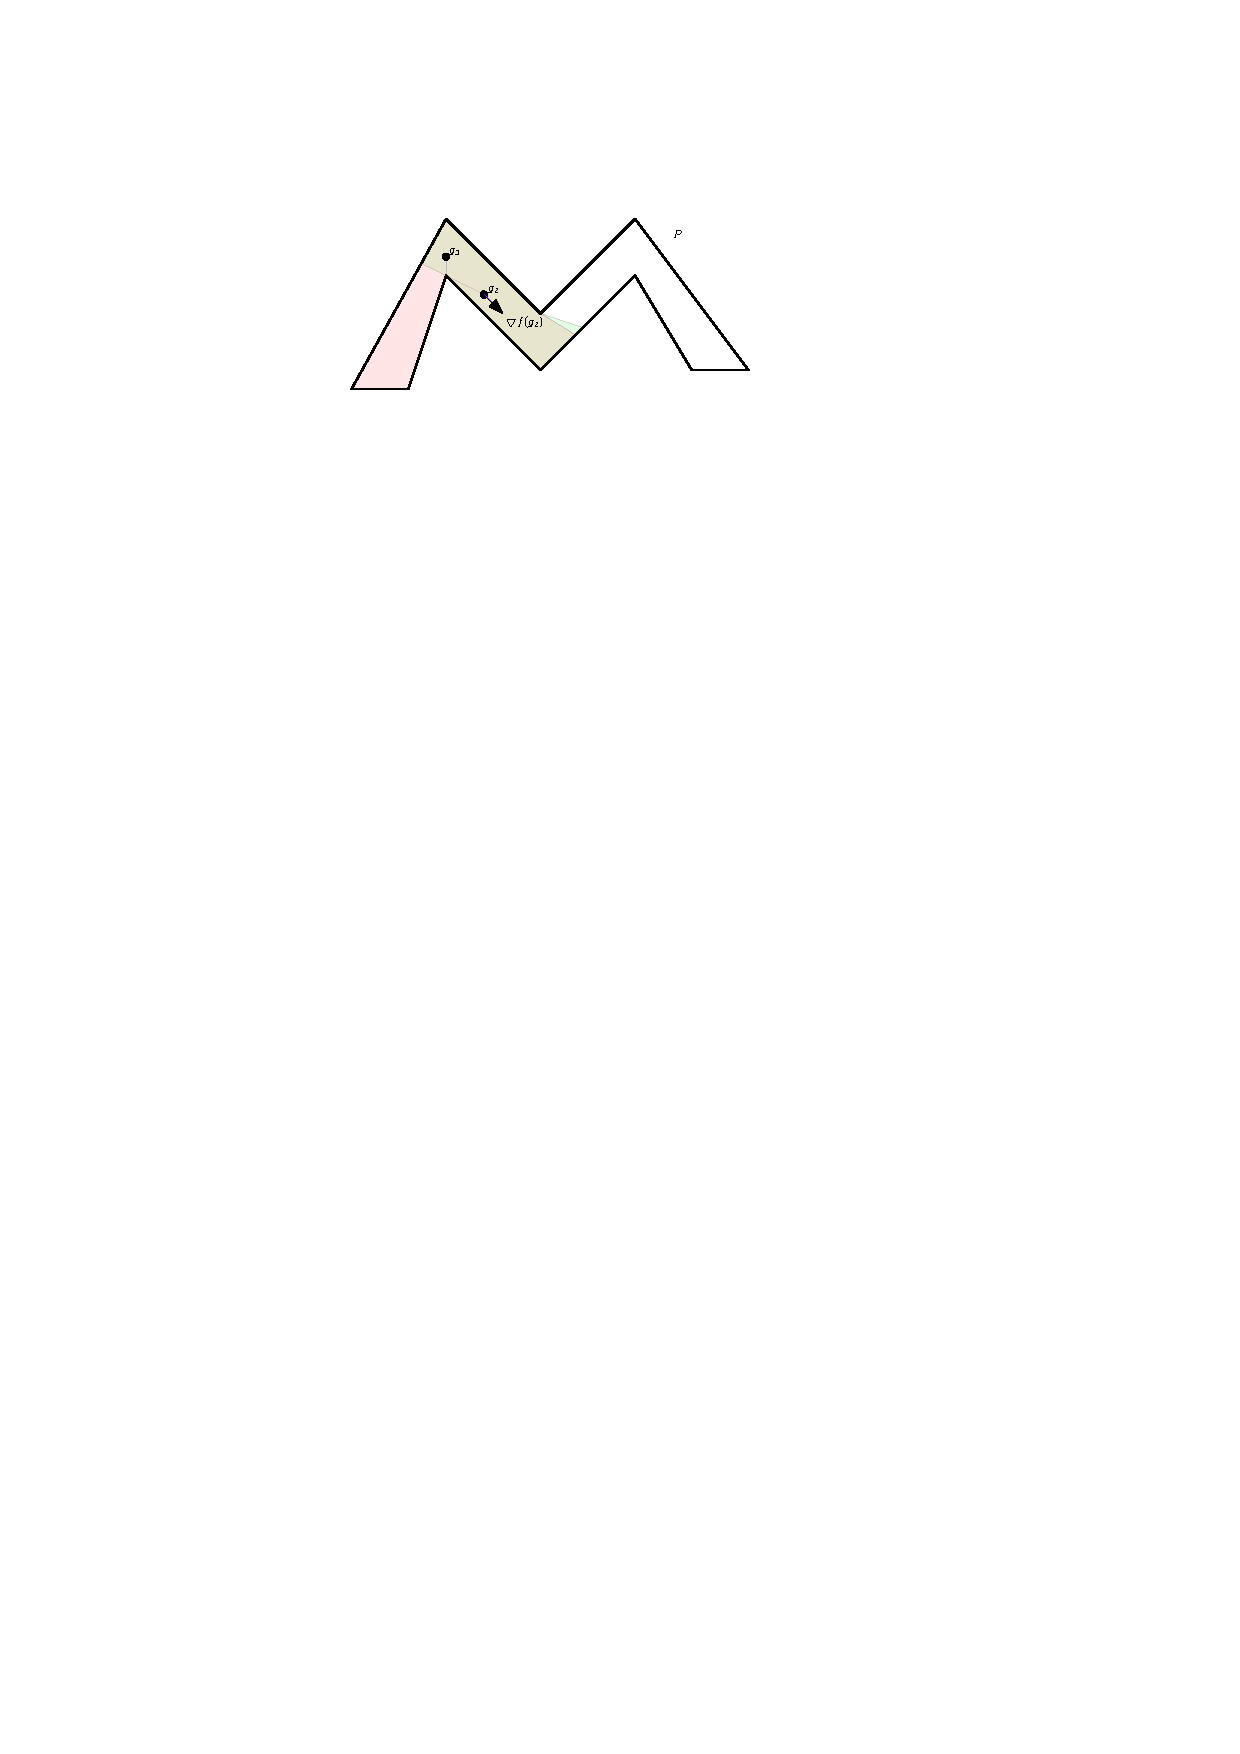
\includegraphics{theory/hidden_gradient2.pdf}
        \caption{Guard $g_1$ had a non-zero movement vector, so we compute the movement vectors of guards $g_2$ and $g_3$ without $g_1$. Guard $g_2$ sees everything that $g_3$ sees, so $g_3$ has movement vector 0. So, the set of guards with a non-zero movement vector is $G_1 = \{g_2\}$.}
        \label{fig:hidden_gradient2}
    \end{subfigure}
    \begin{subfigure}{0.45\textwidth}
        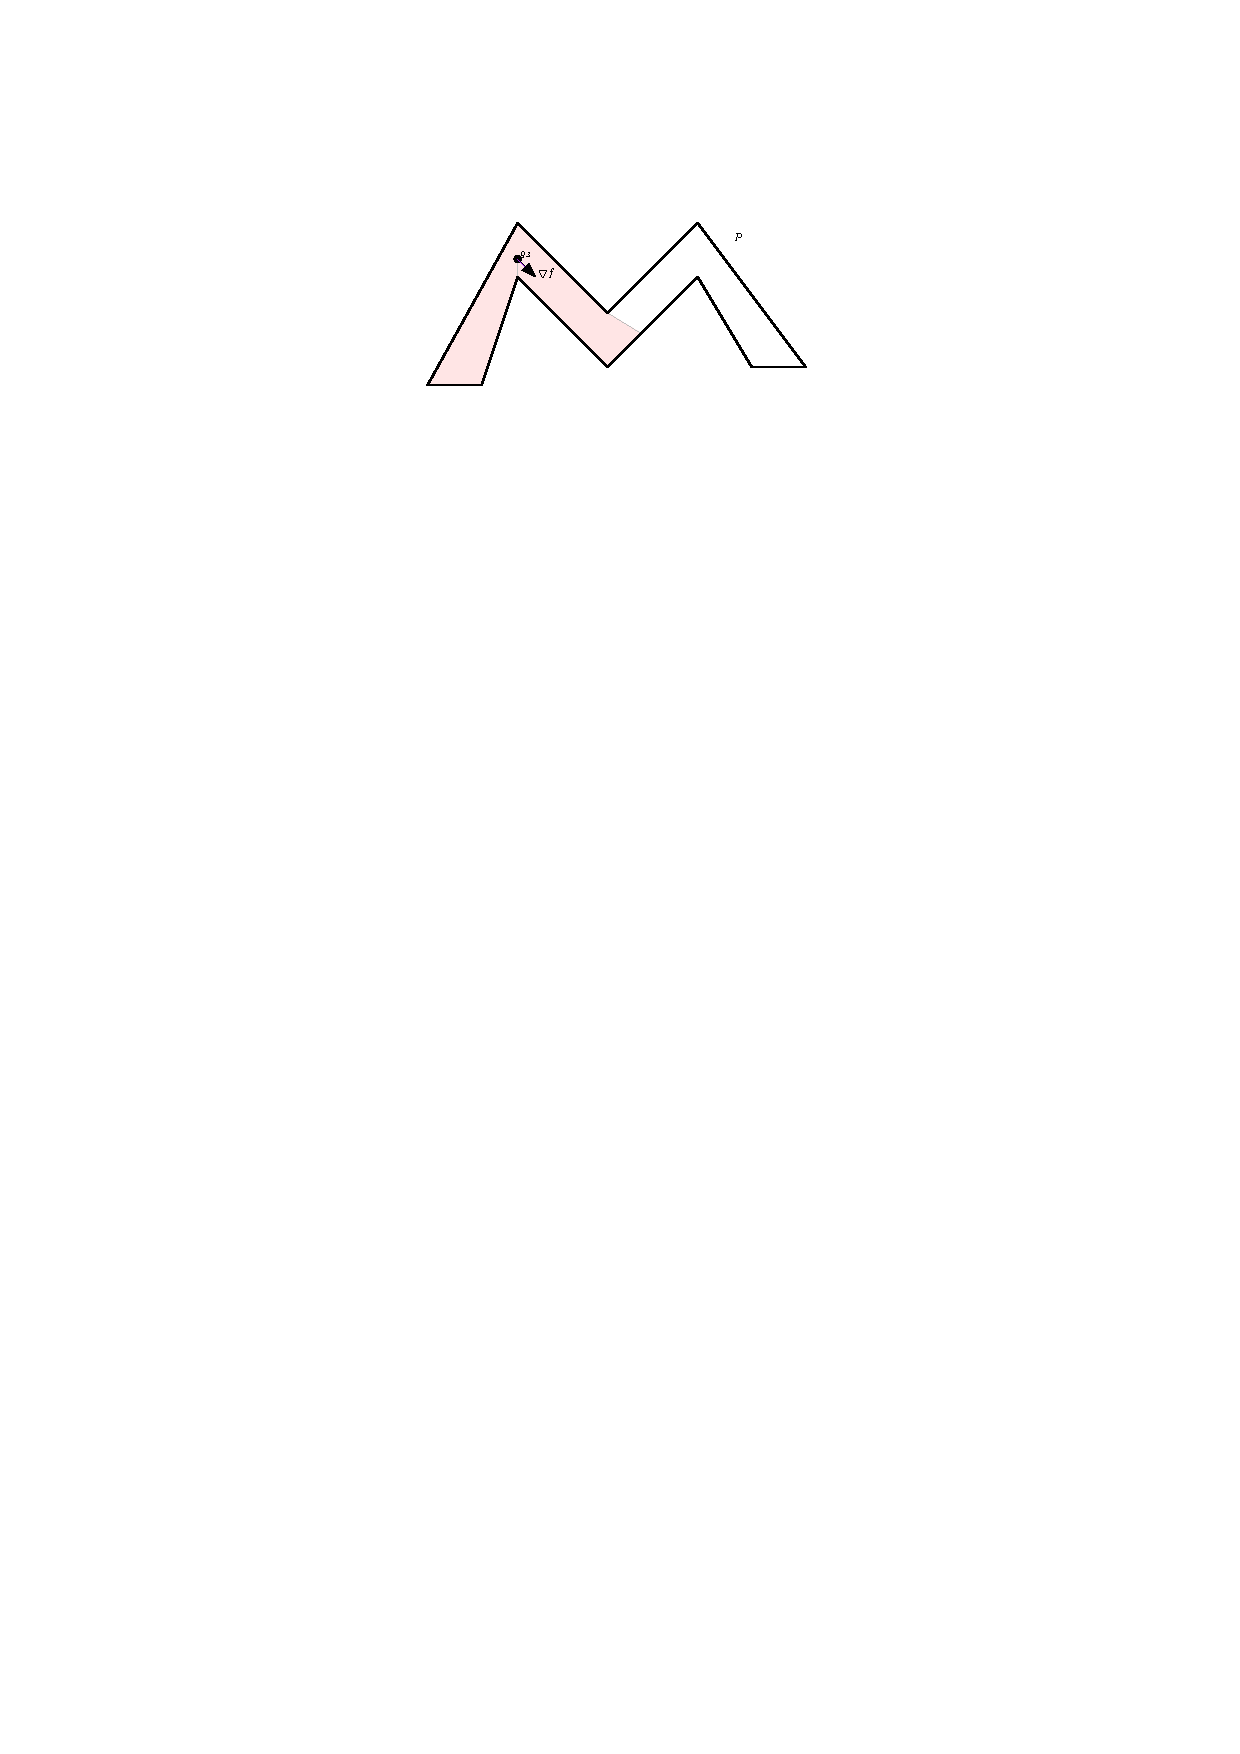
\includegraphics{theory/hidden_gradient3.pdf}
        \caption{Guard $g_2$ had a non-zero movement vector, so we compute the movement vector of guard $g_3$ without $g_2$. Guard $g_3$ has a non-zero movement vector. So, the set of guards with a non-zero movement vector is $G_2 = \{g_3\}$.}
        \label{fig:hidden_gradient3}
    \end{subfigure}
    \hfill
    \begin{subfigure}{0.45\textwidth}
        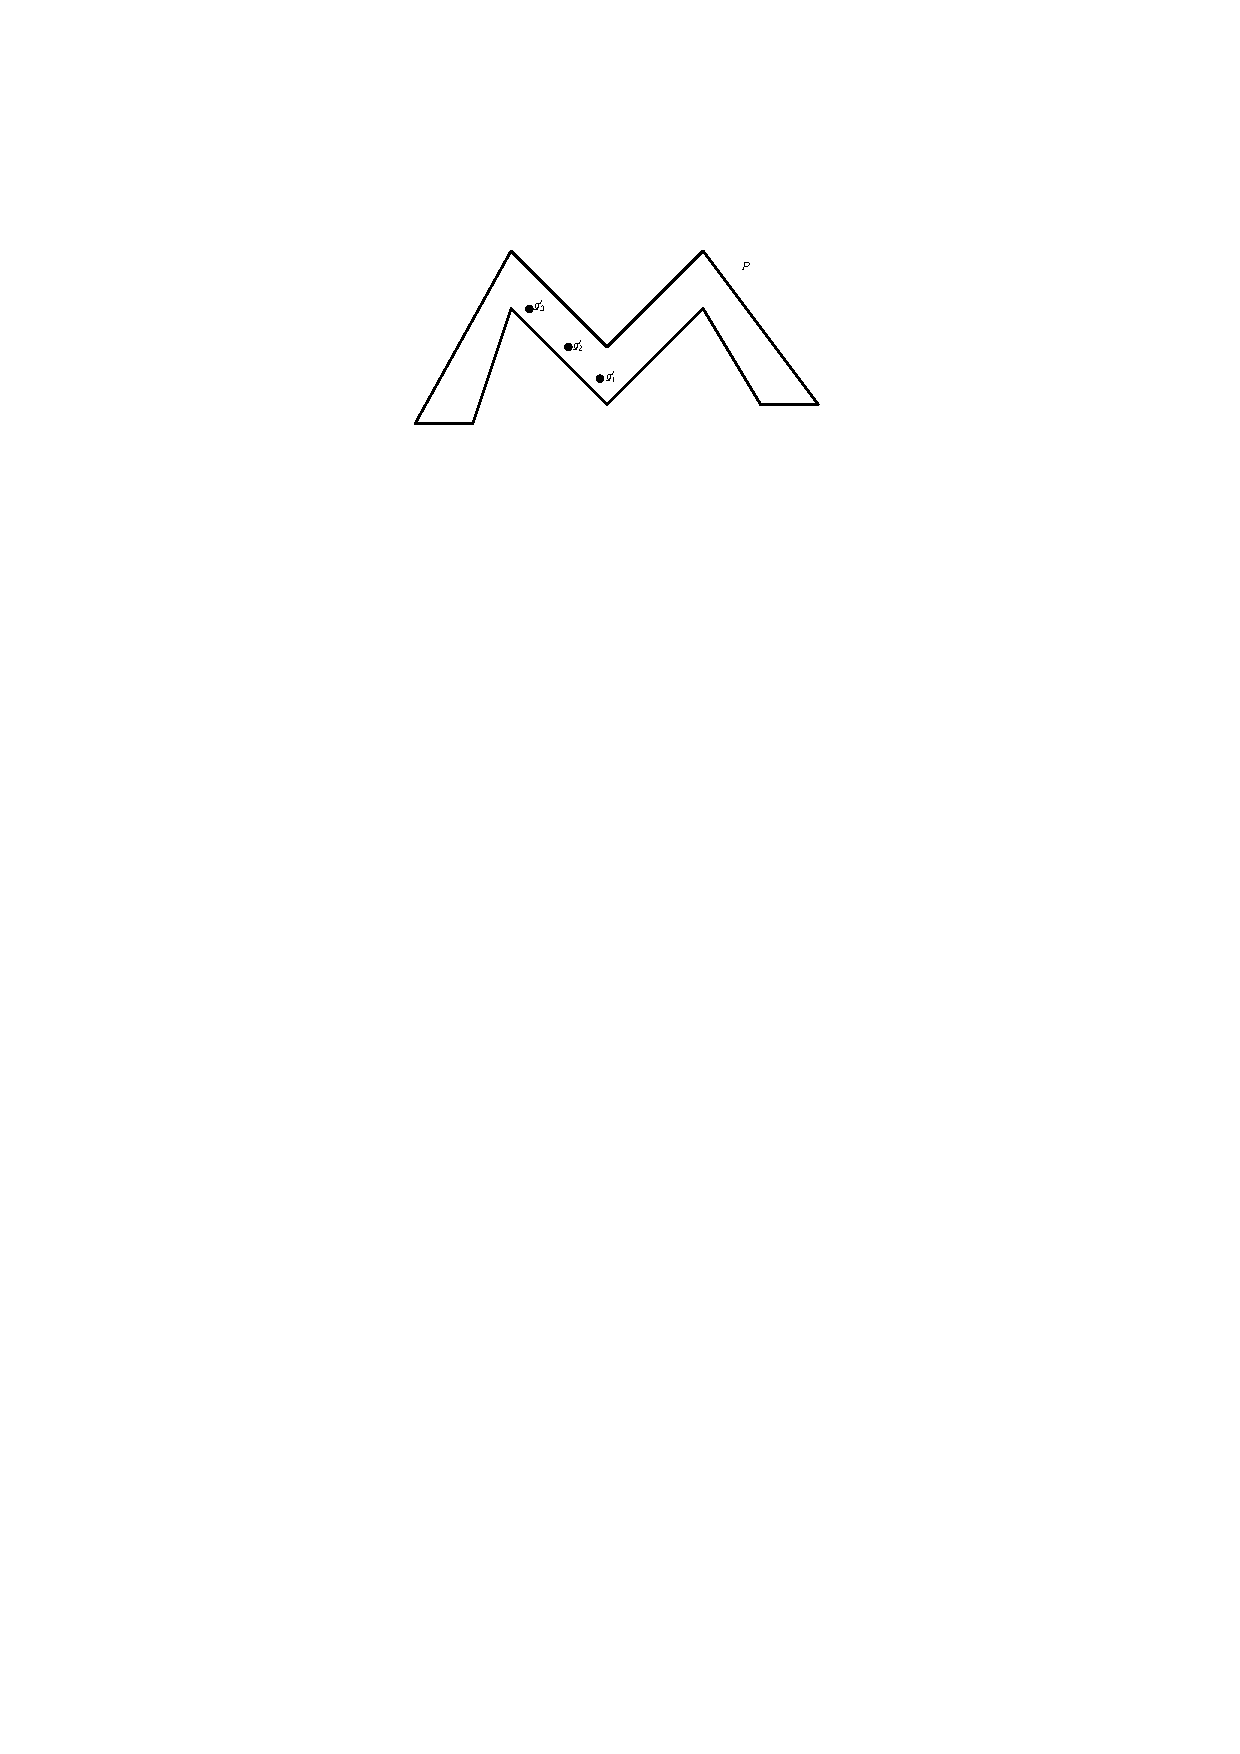
\includegraphics{theory/hidden_gradient4.pdf}
        \caption{The new positions $g'_1, g'_2, g'_3$ of the guards such that $G = G_0 \cup G_1 \cup G_2$.}
        \label{fig:hidden_gradient4}
    \end{subfigure}
    \caption{Example of hidden movement computation for guard set $G = \{g_1, g_2, g_3\}$ in a corridor-like polygon. The visibility areas of each of the guards $g_1, g_2$, and $g_3$ are shown in purple, green and orange, respectively.}
    \label{fig:hidden_gradient}
\end{figure}

The hidden movement heuristic can be generalised. Let $G$ be the complete set of guards. For each step $i$, let $G_i = G \setminus G_{i - 1}$ be the set of guards with a non-zero movement vector after removing the guards with a movement vector from step $i - 1$. The set $G_0$ is the set of guards with a non-zero movement vector before removal of any guards. At the end, the union of all subsets $G_i$ comprises the set of all guards $G = G_0 \cup G_1 \cup ...$.
In this way, all guards  have a non-zero movement vector and make progress.

\subsection{Greedy Initialisation}
\label{sec:greedy}
% - head start
In this section we  introduce another heuristic for our algorithm: \textit{greedy initialisation}. This heuristic sequentially places guards at starting positions in areas that are unseen by other guards. In this way, the algorithm has a head start with a larger covered area than when guards are placed arbitrarily.

Figure \ref{fig:greedy} offers an example of a greedy initialisation. The first guard $g_1$ is arbitrarily placed inside polygon $P$ as shown in Subfigure \ref{fig:greedy1}. Then, guard $g_2$ is arbitrarily placed in an unseen part of $P$, as displayed in Subfigure \ref{fig:greedy2}. In this way, the algorithm gains a head start to continue with the optimisation of the guards' positions.

\begin{figure}[h!]
    \centering
    \begin{subfigure}{0.45\textwidth}
        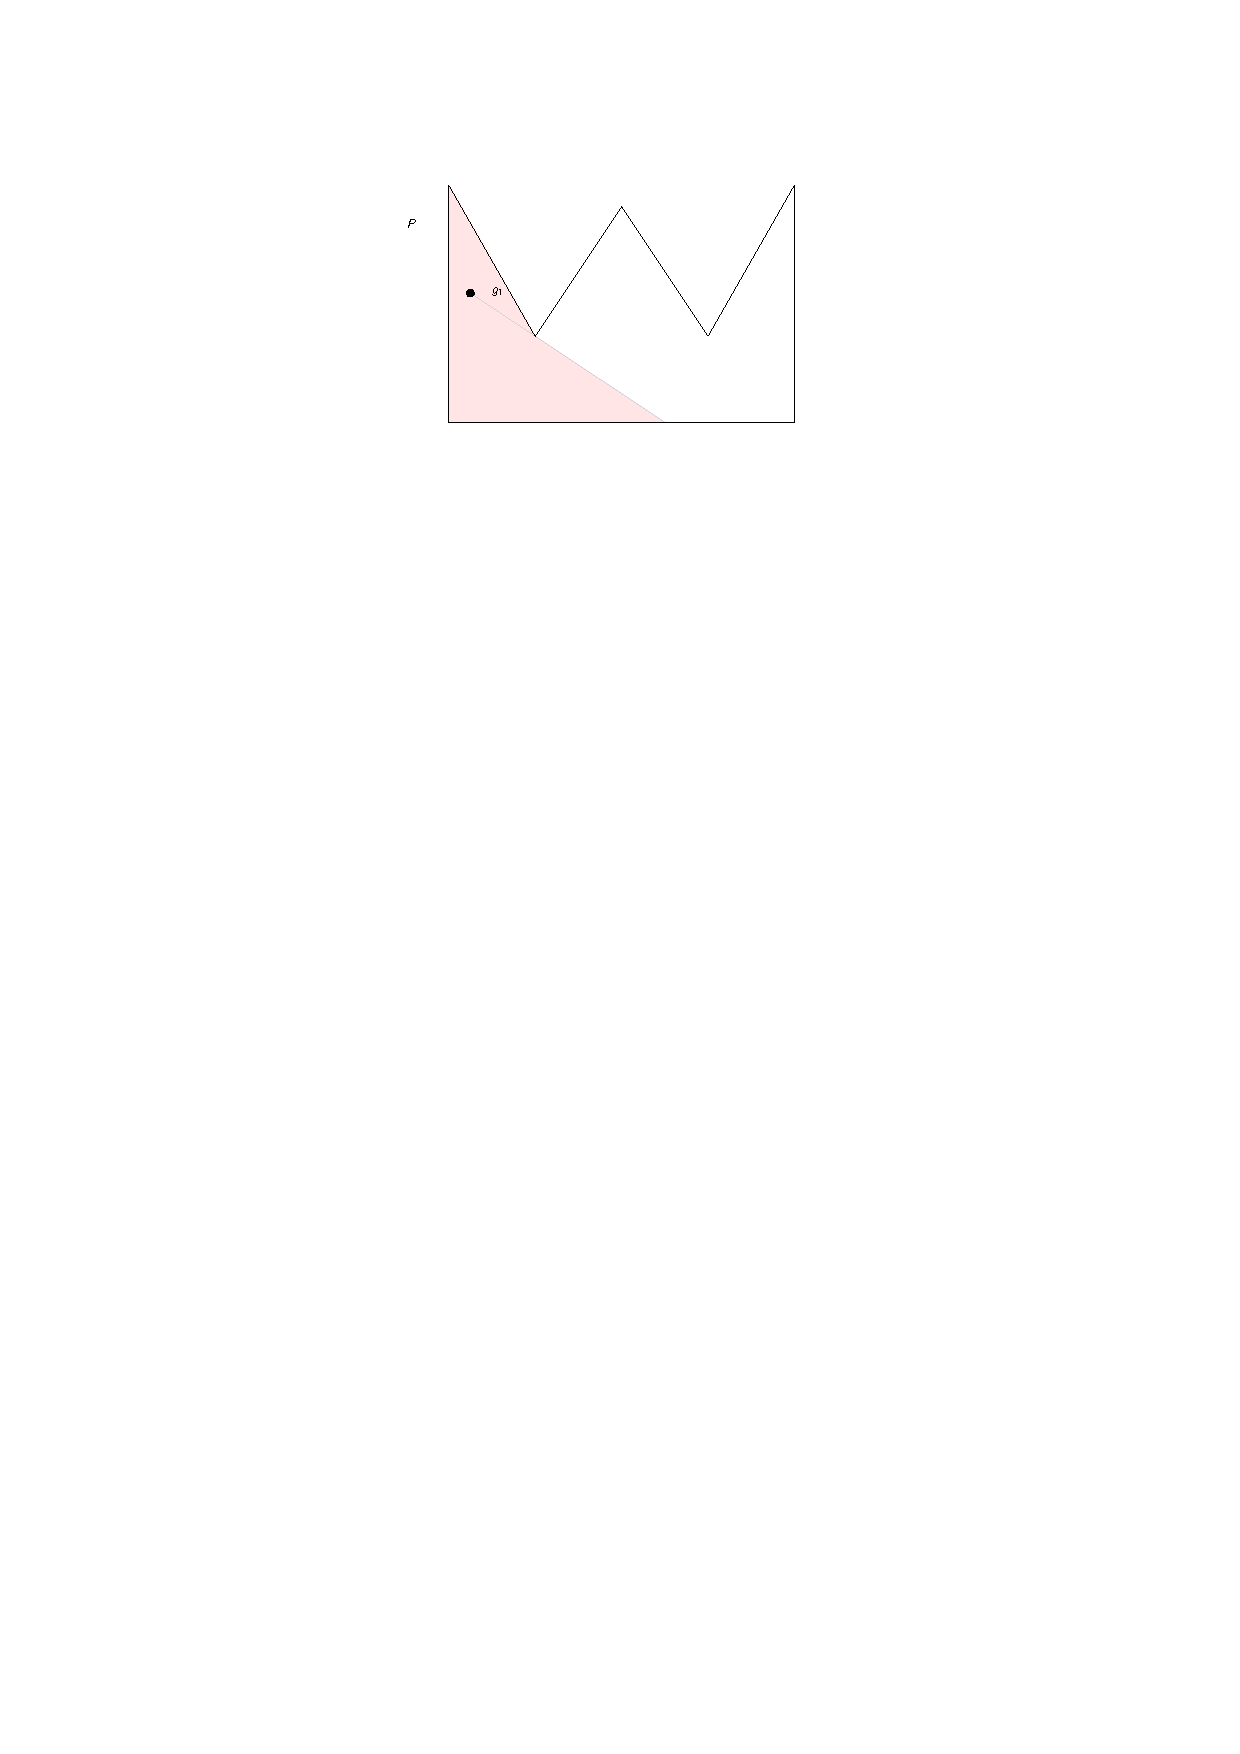
\includegraphics{theory/greedy1.pdf}
        \caption{Guard $g_1$ has been arbitrarily placed inside the polygon $P$.}
        \label{fig:greedy1}
    \end{subfigure}
    \hfill
    \begin{subfigure}{0.45\textwidth}
        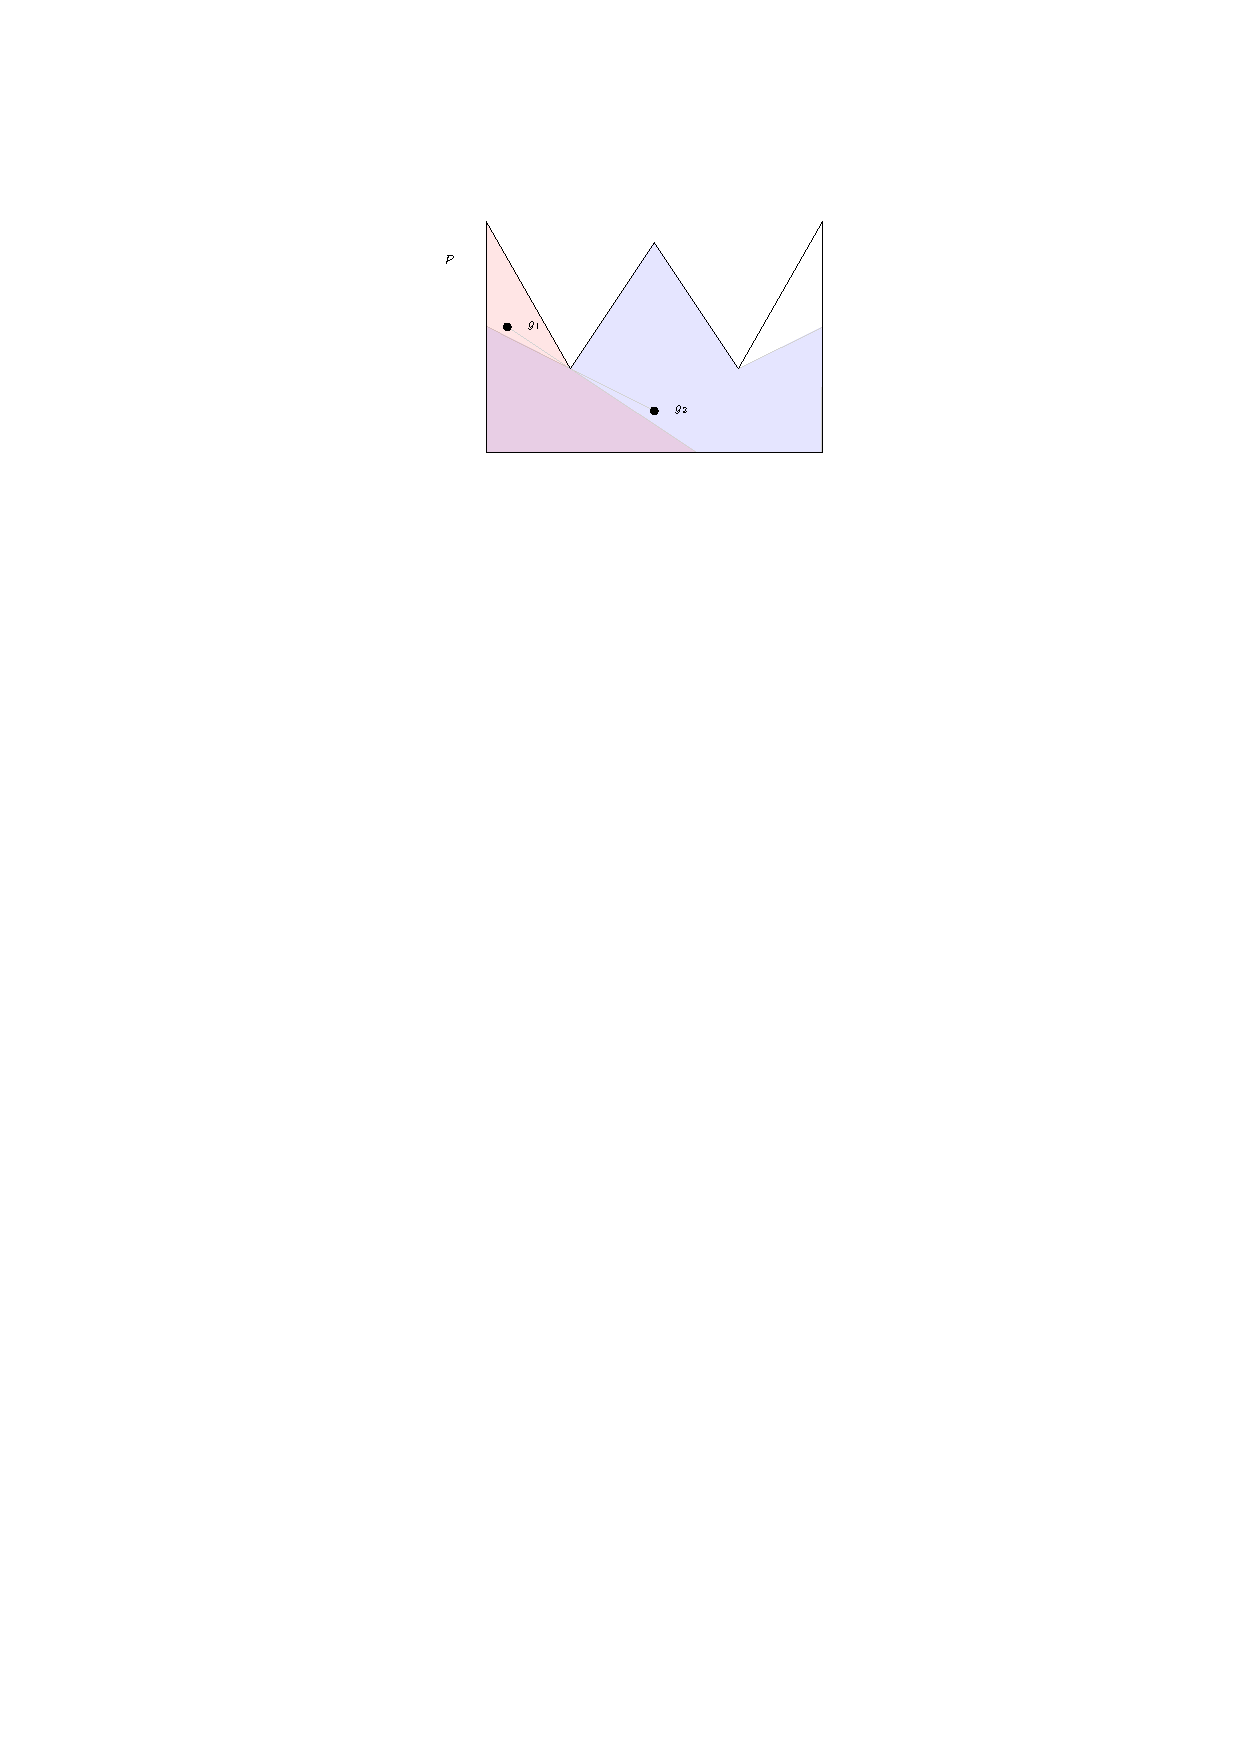
\includegraphics{theory/greedy2.pdf}
        \caption{Guard $g_2$ has been arbitrarily placed inside the polygon $P$, outside the visibility region of guard $g_1$.}
        \label{fig:greedy2}
    \end{subfigure}
    % \begin{subfigure}{0.45\textwidth}
    %     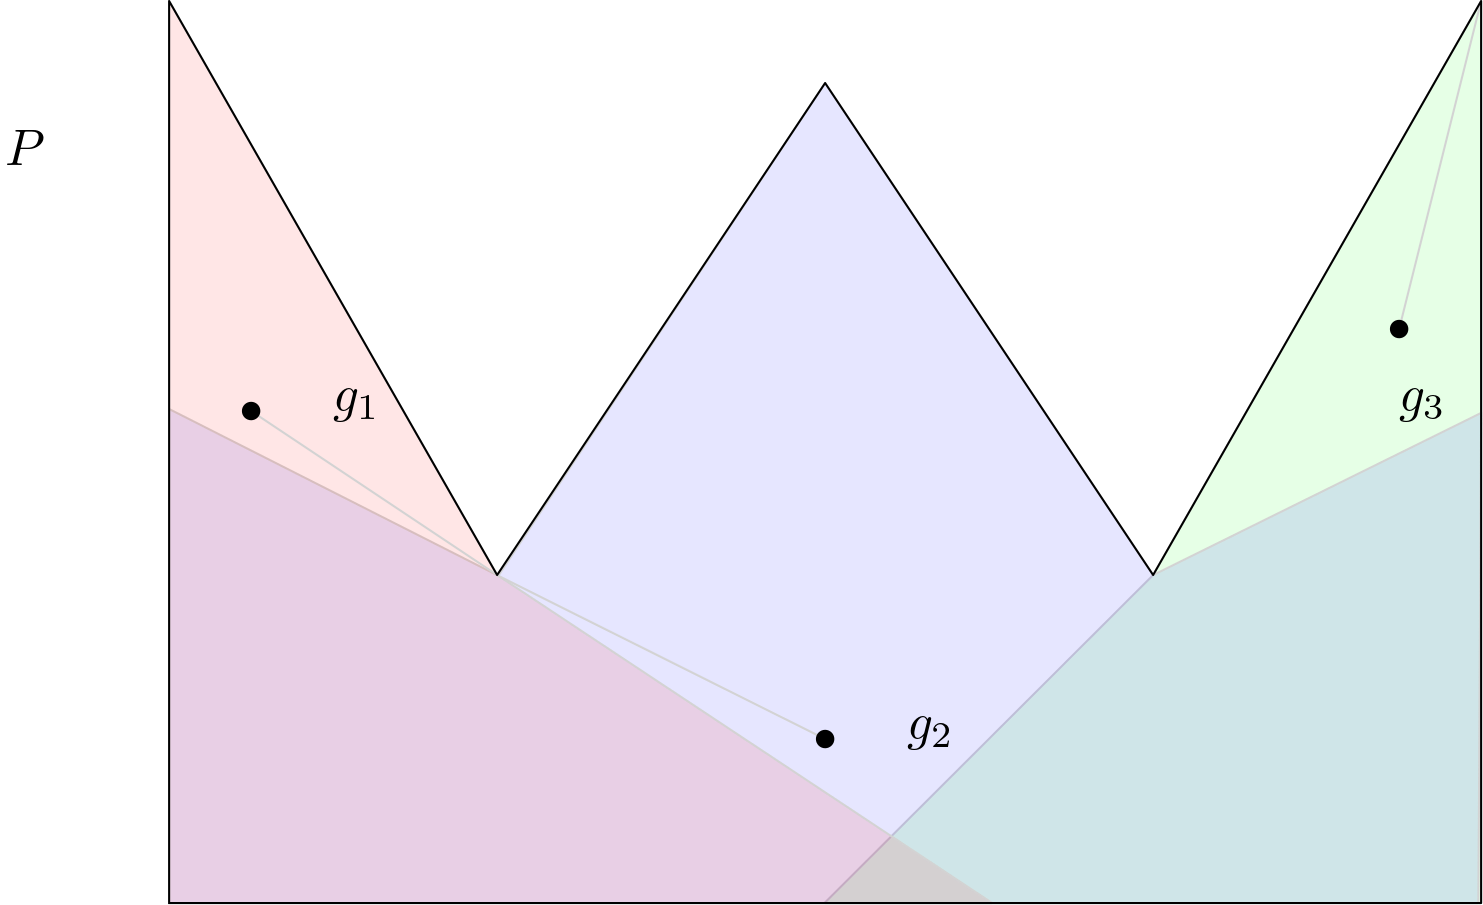
\includegraphics[width = \textwidth]{theory/greedy.png}
    %     \caption{Guard $g_3$ has been arbitrarily placed inside the polygon $P$, outside of the visibility regions of guards $g_1$ and $g_2$.}
    %     \label{fig:greedy3}
    % \end{subfigure}
    \caption{Greedy Initialisation for guards $g_1$ and $g_2$ inside polygon $P$. The visibility regions of the guards are displayed in orange and purple, respectively. In this way, the algorithm gains a head start for optimising the positions of the guards.}
    \label{fig:greedy}
\end{figure}
